%Auteurs : Enes Ulusoy
\documentclass[british,french,11pt, a4paper, openany]{book}

% Règles de bonne pratiques :
% https://fr.wikibooks.org/wiki/LaTeX/Gestion_des_gros_documents
\usepackage{../../Builder/preambule}
\usepackage{multicol}
\usepackage{bm}
% %%%%%%%%%%%%%%%%
%%% Packages %%%
%%%%%%%%%%%%%%%%

%%% Compatibilité %%%
\begingroup\expandafter\expandafter\expandafter\endgroup
\expandafter\ifx\csname IncludeInRelease\endcsname\relax
\usepackage{fixltx2e}
\fi 					% Si version LaTeX < 2015, inclut un fix.

%%% Général %%%
\usepackage[utf8]{inputenc}
\usepackage{babel}
\usepackage{lmodern}
\usepackage[T1]{fontenc}
\addto\extrasfrench{\sisetup{locale = FR,detect-all}} % Switch siunitx en fonction de la langue babel :)
\addto\extrasbritish{\sisetup{locale = UK,detect-all}}
\usepackage{courier}
\usepackage{graphicx}
%\usepackage{cancel}

%%% Tableau %%%
%\usepackage{tabularx} %Permet d'auto dimensionner les tableaux



%%% Bibliographie %%%
%\usepackage[style=alphabetic,backend=biber]{biblatex}
\usepackage[autostyle]{csquotes}
%\DeclareNameAlias{sortname}{last-first}
%\DeclareFieldFormat{url}{\space\url{#1}}
%\DeclareNameAlias{labelname}{last-first}
%\addbibresource{sample.bib}


%%% Graphiques %%%
%\usepackage{tikz}
%\usepackage{pgfplots}
%\usepackage{circuitikz}

%%% Mise en page %%%
\usepackage{mathtools}
\usepackage{amssymb}
\usepackage{bbm}
\usepackage{amsthm}
%\usepackage[tt]{titlepic}% Centre le titre
%\usepackage{fancyhdr}   % Permet de modifier l'entête & footer
\usepackage{caption}     % Permet d'ajouter des légendes en images sans les mettre en float + dans la marge + ref vers le haut de l'envirronement
\usepackage{wrapfig}
\usepackage{fullpage}
%\usepackage{multicol}   % pour les liste sur plusieurs colonnes
%\usepackage{subfigure}  % alligne deux images cote a cote
\usepackage{float}      %permet de mettre du texte entre les figures grace a [H]. Génial! 
\usepackage{eso-pic}    % Fond d'écran page de garde
\usepackage{adjustbox}  % Empêche les box de sortir de la page


%%% Math %%%
%\usepackage{delarray} % Belles matrices
\usepackage{siunitx}


%%% Codes %%%
%\usepackage{listings}
%\usepackage[final]{pdfpages} %% Inclusion fichier pdf

%% Reference
\usepackage{hyperref}
%\renewcommand*{\figureautorefname}{fig.}
%\def\appendixautorefname{annexe}
%\def\tableautorefname{tab.}
%\renewcommand*{\chapterautorefname}{ch.}
%\newcommand{\subfigureautorefname}{\figureautorefname}



%%%%%%%%%%%%%%%%%
%%% Commandes %%%
%%%%%%%%%%%%%%%%%

%%% Physique %%%
\newcommand{\cst}{\text{cst}}
\newcommand{\D}{\partial}
\newcommand{\E}{\vec E}
\newcommand{\B}{\vec B}
\newcommand{\F}{\vec F}
\newcommand{\modu}[1]{|$#1$|}

%%% Math %%%
\newcommand{\oiint}{\int\!\!\!\!\!\!\! \:\!\subset\!\!\supset\!\!\!\!\!\!\!\int}
\newcommand{\rot}{\operatorname{\vec{rot}}}
\newcommand{\divv}{\operatorname{div}}
\newcommand{\phas}[1]{\underline{#1}}
\newcommand{\RE}{\text{Re}}
\newcommand{\ft}{\overset{\mathcal{F}}{\longleftrightarrow}}
\newcommand{\lt}{\overset{\mathcal{L}}{\longleftrightarrow}}
\newcommand{\DS}{\displaystyle}
\newcommand{\Tr}{\operatorname{Tr}}



%% Box
\shorthandon{:}
\newcommand{\theor}[1]{\adjustbox{minipage=\linewidth-2\fboxsep-2\fboxrule,fbox}{\textsc{\iflanguage{british}{Theorem}{Théorème}: }#1}}
\newcommand{\defi}[1]{\adjustbox{minipage=\linewidth-2\fboxsep-2\fboxrule,fbox}{\textsc{\iflanguage{british}{Definition}{Définition}: }#1}}
\newcommand{\lemme}[1]{\adjustbox{minipage=\linewidth-2\fboxsep-2\fboxrule,fbox}{\textsc{\iflanguage{british}{Lemma}{Lemme}: }#1}}
\newcommand{\prop}[1]{\adjustbox{minipage=\linewidth-2\fboxsep-2\fboxrule,fbox}{\textsc{\iflanguage{british}{Property}{Propriété}}\\ #1}}
\newcommand{\proposition}[1]{\adjustbox{minipage=\linewidth-2\fboxsep-2\fboxrule,fbox}{\textsc{Proposition}\\#1}}
\newcommand{\cadre}[1]{\adjustbox{minipage=\linewidth-2\fboxsep-2\fboxrule,fbox}{#1}}
\newcommand{\retenir}[1]{\adjustbox{minipage=\linewidth-2\fboxsep-2\fboxrule,fbox}{\textbf{\textit{\textsc{\iflanguage{british}{To remember}{À retenir}}: }}#1}}

\newcommand{\corollaire}[1]{\bigbreak\begin{tabular}{||c}
	\begin{minipage}{\textwidth}
		\textsc{\iflanguage{british}{Corollary}{Corollaire}: } \textit{#1}
	\end{minipage}
	\end{tabular}}
\newcommand{\exemple}[1]{\bigbreak\begin{tabular}{|c}
	\begin{minipage}{\textwidth}
		\textsc{\iflanguage{british}{Example}{Exemple}: } #1
	\end{minipage}%
	\end{tabular}}%
\shorthandoff{:}
    

%\pagestyle{headings} % Titre du ch et numéro page dans l'entete
%\renewcommand{\proofname}{Démonstration}
%\addto\captionsfrench{\def\tablename{Tableau}}


%%% Background %%%
\newcommand\BackgroundPic{%
	\put(0,0){%
		\parbox[b][\paperheight]{\paperwidth}{%
			\vfill
			\centering
			\includegraphics[width=\paperwidth,height=\paperheight,%
			keepaspectratio]{../../Builder/ulb.jpg}%
			\vfill
}}}

%%% Annexes Cedu %%%
%\usepackage{calrsfs}
%\DeclareMathAlphabet{\pazocal}{OMS}{zplm}{m}{n}
\usepackage{fourier-orns}

\setlength{\parindent}{0pt} 

%%% Attributs %%%
\newcommand*{\NomduCours}[2]{\def\cours{#1}\def\memo{#2}}
\newcommand*{\annee}[2]{\def\adebut{#1}\def\afin{#2}}

\newcounter{auteurcnt}
\newcommand\addauteur[2]{%
	\stepcounter{auteurcnt}%
	\csdef{auteur\theauteurcnt}{\mbox{#1~\textsc{#2}}}}
\newcommand\getauteur[1]{%
	\csuse{auteur#1}}

\newcounter{illustrateurcnt}
\newcommand\addillustrateur[2]{%
	\stepcounter{illustrateurcnt}%
	\csdef{illustrateur\theillustrateurcnt}{\mbox{#1~\textsc{#2}}}}
\newcommand\getillustrateur[1]{%
	\csuse{illustrateur#1}}

\newcounter{rappeltheocnt}
\newcommand\addrappeltheo[2]{%
	\stepcounter{rappeltheocnt}%
	\csdef{rappeltheo\therappeltheocnt}{\mbox{#1~\textsc{#2}}}}
\newcommand\getrappeltheo[1]{%
	\csuse{rappeltheo#1}}

\newcounter{professeurcnt}
\newcommand\addprofesseur[2]{%
	\stepcounter{professeurcnt}%
	\csdef{professeur\theprofesseurcnt}{\mbox{#1~\textsc{#2}}}}
\newcommand\getprofesseur[1]{%
	\csuse{professeur#1}}

\newcounter{iter}
% Attributs
\NomduCours{Numerical methods in aerothermodynamics}{MECA-H-407}
\addauteur{Enes}{Ulusoy}
\addprofesseur{Gérard}{Degrez}
\annee{2016}{2017}
\renewcommand{\theor}[1]{\adjustbox{minipage=\linewidth-2\fboxsep-2\fboxrule,fbox}{\textsc{}#1}}
\newcommand{\uinf}{u_\infty}

\newcommand{\wrapfig}[5]{%
\begin{wrapfigure}[#1]{#2}{#3cm}%
\vspace{-5mm}%
\includegraphics[scale=#4]{#5}%
\captionof{figure}{}%
\label{#5}%
\end{wrapfigure}%
}

\newcommand{\minifig}[6]{
\begin{center}%
	\begin{minipage}{#5\textwidth}%
	\includegraphics[scale=#3]{#1}%
	\captionof{figure}{}%
	\label{#1}%
	\end{minipage}%
	\begin{minipage}{#6\textwidth}%
	\includegraphics[scale=#4]{#2}%
	\captionof{figure}{}%
	\label{#2}%
	\end{minipage}%
	\end{center}
}

% Document
\begin{document}
\selectlanguage{british}
\def\equationautorefname~#1\null{%
		(#1)\null
	}
%%%%%%%%%%%%%%%%%
% Préliminaires %
%%%%%%%%%%%%%%%%%
\frontmatter
\AddToShipoutPicture*{\BackgroundPic}

\begin{titlepage}
	\begin{center}	
			
		\newcommand{\HRule}{\rule{\linewidth}{0.5mm}}   			            %Titre en gros
		\includegraphics[width=0.55\textwidth]{../../Builder/titlepage/logo.pdf}~\\[1cm]				%Logo
			
			\textsc{\LARGE Université Libre de Bruxelles}\\[1.5cm]
			\textsc{\Large \iflanguage{british}{Summary}{Synthèse}}\\[0.5cm]
			
			\HRule \\[0.4cm]
			{ \huge \bfseries \cours \ \\\memo \\[0.4cm] }
			
			
			\HRule \\[1.5cm]
			\begin{minipage}[t]{0.6\textwidth}
				\begin{flushleft}%\large
					\emph{\iflanguage{british}{Author}{Auteur}\ifnum\theauteurcnt>1 s\fi:}\\
					\whileboolexpr
					{ test {\ifnumcomp{\value{iter}}{<}{\theauteurcnt}} }%
					{\stepcounter{iter}\getauteur{\theiter}\\}
					\setcounter{iter}{0}%
					\ifnum\theillustrateurcnt>0%
					\ \\
					\emph{Illustrations:}\\
					\whileboolexpr
					{ test {\ifnumcomp{\value{iter}}{<}{\theillustrateurcnt}} }%
					{\stepcounter{iter}\getillustrateur{\theiter}\\}%
					\setcounter{iter}{0}%
					\fi%
					\ifnum\therappeltheocnt>0%
					\ \\
					\emph{\iflanguage{british}{Reminders}{Rappels théoriques}:}\\
					\whileboolexpr
					{ test {\ifnumcomp{\value{iter}}{<}{\therappeltheocnt}} }%
					{\stepcounter{iter}\getrappeltheo{\theiter}\\}%
					\setcounter{iter}{0}%
					\fi%
				\end{flushleft}
			\end{minipage}%
			\begin{minipage}[t]{0.25\textwidth}
				%\begin{flushright}
				%\large
				\emph{\iflanguage{british}{Professor}{Professeur}\ifnum\theprofesseurcnt>1 s\fi:}
				\whileboolexpr
				{ test {\ifnumcomp{\value{iter}}{<}{\theprofesseurcnt}} }%
				{\\ \stepcounter{iter}\getprofesseur{\theiter}}%
				\setcounter{iter}{0}%
				%\end{flushright}
			\end{minipage}
			
			\vfill
			
			% Bottom of the page
			{\large \iflanguage{british}{Year}{Année} \adebut~-~\afin}
			
		\end{center}
	\end{titlepage}

\ \\[2cm]
{\Huge \bfseries Appel à contribution}\\[5mm]
\subsection*{Synthèse Open Source}
\begin{wrapfigure}[5]{l}{4.5cm}
	\includegraphics[scale=0.5]{../../Builder/git.png}
\end{wrapfigure}
Ce document est grandement inspiré de l’excellent cours donné 
par \ifnum\theprofesseurcnt=1 \getprofesseur{1} \else\whileboolexpr
{ test {\ifnumcomp{\value{iter}}{<}{\theprofesseurcnt-2}} }%
{\stepcounter{iter}\getprofesseur{\theiter}, }%
\stepcounter{iter}\getprofesseur{\theiter} et \stepcounter{iter}\getprofesseur{\theiter} \fi%
 à l’EPB (École Polytechnique de Bruxelles), faculté de l’ULB (Université 
Libre de Bruxelles). Il est écrit par les auteurs susnommés avec l’aide de tous les autres étudiants 
et votre aide est la bienvenue ! En effet, il y a toujours moyen de l’améliorer surtout que si le 
cours change, la synthèse doit être changée en conséquence. On peut retrouver le code source à l’adresse 
suivante
\begin{center}
	\url{https://github.com/nenglebert/Syntheses}
\end{center}\bigskip
Pour contribuer à cette synthèse, il vous suffira de créer un compte sur \textit{Github.com}. De
légères modifications (petites coquilles, orthographe, ...) peuvent directement être faites sur le
site ! Vous avez vu une petite faute ? Si oui, la corriger de cette façon ne prendra que quelques 
secondes, une bonne raison de le faire ! \bigskip

Pour de plus longues modifications, il est intéressant de disposer des fichiers : il vous 
faudra pour cela installer \LaTeX, mais aussi \textit{git}. Si cela pose problème, nous sommes 
évidemment ouverts à des contributeurs envoyant leur changement par mail ou n’importe quel autre 
moyen.\bigskip

Le lien donné ci-dessus contient aussi un \texttt{README} contenant de plus amples informations, 
vous êtes invités à le lire si vous voulez faire avancer ce projet ! 

\subsection*{Licence Creative Commons}
\begin{wrapfigure}[3]{r}{2.8cm}
	\vspace{-5mm}
	\includegraphics[scale=0.17]{../../Builder/CC}
\end{wrapfigure}
Le contenu de ce document est sous la licence Creative Commons : \textit{Attribution-NonCommercial-ShareAlike 
4.0 International (CC BY-NC-SA 4.0)}. Celle-ci vous autorise à l'exploiter pleinement, compte-
tenu de trois choses :
\begin{enumerate}
	\item \textit{Attribution} ; si vous utilisez/modifiez ce document vous devez signaler le(s) nom(s)
	      de(s) auteur(s).
	\item \textit{Non Commercial} ; interdiction de tirer un profit commercial de l’œuvre sans 
	      autorisation de l'auteur 
	\item \textit{Share alike} ;  partage de l’œuvre, avec obligation de rediffuser selon la même 
	      licence ou une licence similaire
\end{enumerate}
Si vous voulez en savoir plus sur cette licence :
\begin{center}
	\url{http://creativecommons.org/licenses/by-nc-sa/4.0/}
\end{center}

\begin{flushright}
	\textbf{Merci ! }
\end{flushright}
\tableofcontents
%Si abstract, \input ici

%%%%%%%%%%%%%%%%%%%%%
% Contenu principal %
%%%%%%%%%%%%%%%%%%%%%
\mainmatter


\chapter*{Introduction}

Fluid dynamics is based on continuity hypothesis, all quantities can be expressed as a continuous function of time and space coordinates. The governing equations are partial differential equations. Because of the geometrical complexity of the domain and of the equations, we need strategies. The first one is to forget about the equations and to rely on experiments. The second is to consider simplified cases, and approximate theoretical analytic solutions (aerodynamics). The third approach is numerical approach. Disadvantages and advantages of the different methods can be listed as: \\

\begin{itemize}
\item[•] \textbf{Experimental:} the advantage is that it is the most realistic, but requires equipment, there are scale problems (similarity), interferences (tests in finite space), measurement difficulties and operating costs.
\item[•] \textbf{Theoretical}: the advantage is that we have a mathematical expression and we don't have to repeat calculus, but it is restricted to simple geometries and linear problems. 
\item[•] \textbf{Numerical}: the advantages are that we can dead with complex geometries, non linear problems and unsteady problems, but there are truncation errors, problems with boundary conditions like the finite space in experiment and the computation cost. \\
\end{itemize}

In reality these approaches are complementary. We can use the second method to simplify the numerical computations, crucial for example for costly operations like computations on turbulence. The evolution of numerical cost over the past 40 years has been particularly impressive, cost decreased dramatically. In the other hand, the experimental cost tends to increase (technical personal, material,…). Nowadays we can measure many things impossible to measure before. This explains why the numerical computations have spread incredibly. \\

The design relies mainly on the numerical methods and less on the experimental testing, but it is still needed to confirm the data. We can use the numerical methods in many fields and we could call this « numerical physics ». We should deal with this in a single course of computational method and then to specialize it to the specific disciplines. An approximate solution to a problem is some kind of mathematical entity, an object, which depends on a finite number of real parameters, and which constitutes a representation of the continuous field under study. The numerical solution belongs to a finite dimension space whereas the theoretical to an infinite. \\

There are different types of numerical representation:

\begin{itemize}
\item[•] \textbf{Discrete:} collection of either point values (samples of the solutions) or subdomain averages. We are not able to give an exact solution on basis of these points, but rather an estimation.
\item[•] \textbf{Functional:} the solution is expressed as a function $u*(x) = f(x,a_i)$, depending on a set of variables. Most of the time the dependence is linear: $u* = \sum_{i=1}n a_i v_i(x)$ where $v_i(x)$ are a priori specified functions. \\
\end{itemize}

Ones we have chosen the numerical representation method, we have to generate a system of algebraic equations linking the parameters from the representation and the governing equations. The last step is to solve the system. The step of generating the equations system is called \textbf{discretization}. For one problem, several discretizations are possible. Some examples are given, consult the syllabus for more details. 
\chapter{Interaction des particules chargées avec la matière : considérations de base}
\section{Introduction}
Il existe trois types de rayonnements ionisants (\textit{ionizing radiations})
\begin{enumerate}
\item Les particules chargées
\begin{itemize}
\item Électron, positron, ions, \dots
\end{itemize}
\item Les photons (particules neutres sans masses)
	\begin{itemize}
	\item Les $\gamma$ (origine \textbf{nucléaire})
	\item Les $X$ (origine atomique)
	\end{itemize}
\item Neutrons (particules neutres)
\end{enumerate}
Notons que ce qui fait vraiment la différence entre un $\gamma$ et un $X$ est le mode 
d'émission et non pas l'énergie (conséquence).\\

Pour chacun de ces types de rayonnement, il existe un mécanisme d'interaction particulier
avec la matière\footnote{\textit{Assemblage d'atomes isolés sans interaction entre-eux : 
gaz d'atome}. Il s'agit de la définition de ce cours, qui évoluera au fil des chapitres}. 
\begin{itemize}
\item[$\bullet$] Les particules chargées interagissent par interactions coulombienne 
(noyaux et électrons), les collisions sont donc fréquentes et on peut considérer que 
l'énergie est perdue de façon (quasi-)continue. La particule s'arrête ainsi à distance 
finie dans la matière de sorte à ce qu'on puisse définir un "parcours" (\textit{range}) 
de celle ci  : de tels rayonnements sont \textit{directement} ionisants
\item[$\bullet$] Les particules neutres (pas d'interaction coulombienne) ont une 
probabilité de traverser la matière sans interactions, il n'est donc pas possible de 
définir un range. Elles peuvent par contre déposées de l'énergie à des particules 
chargées qui vont causés une ionisation : de tels rayonnements sont \textit{indirectement} 
ionisants
\end{itemize}
Les interactions d'un rayonnement avec la matière peut modifier l'état du rayonnement 
(absorbé, dévié, \dots) et aussi l'état de la matière (excités, ionisés,\dots).

\newpage
\subsection{Interaction des particules chargées avec la matière}
	\begin{wrapfigure}[7]{l}{6cm}
	\vspace{2mm}
	\includegraphics[scale=0.4]{ch1/image1.png}
	\captionof{figure}{Trajectoire d'une particule chargée}
	\end{wrapfigure}
Comme annoncé ci-dessus, les particules chargées subissent des collisions 
coulombiennes\footnote{Les réactions nucléaires sont laissées de côté.} avec :
\begin{description}
\item[Les noyaux (rare)] : cause une importante perte d'énergie et une grande déviation
angulaire
\item[Les électrons (fréquent)] : cause des excitations/ionisations se traduisant par des
faibles pertes d'énergie et déviations angulaires
\end{description}\ \\

	\begin{wrapfigure}[7]{r}{6cm}
	\vspace{-9mm}
	\includegraphics[scale=0.4]{ch1/image2.png}
	\captionof{figure}{ }
	\end{wrapfigure}
Chaque collision cause alors une perte d'énergie $T_j$, causés par un grand nombre de 
projectiles $N$ qui suivent $N$ histoires propres : le nombre de collision étant très 
important, les fluctuations sont faibles et il devient possible de définir des quantités
moyennes.\\

Pour introduire ces valeurs moyennes, il faut avant tout introduire la notion de 
\textbf{section efficace}.\ \\

\cadre{La \textbf{section efficace} est l'aire fictive que doit avoir une particule incidente
pour reproduire la probabilité de collision observée avec une particule cible.}\ \\

	\begin{wrapfigure}[7]{l}{6cm}
	\vspace{-5mm}
	\includegraphics[scale=0.5]{ch1/image3.png}
	\captionof{figure}{ }
	\end{wrapfigure}
Il existe plusieurs sortes de section efficace. Pour s'en rendre compte, définissons ce
qu'est une collision. Il s'agit de \textit{l'interaction entre une particule incidente et une particule cible qui implique un effet spécifique mesurable}. Ainsi, la section efficace ne 
dépend pas que des particules incidentes/cibles et de leur vitesse \textbf{mais aussi} de l'effet
physique !\\
\ \\

Sur le grand nombre d'interaction existant, on peut s'intéresser à une perte d'énergie 
(section efficace différentielle en énergie $d\sigma/dE$) ou à une émission dans une 
direction donnée ((section efficace différentielle en énergie $d\sigma/d\Omega$).\\

	\begin{wrapfigure}[7]{r}{5cm}
	\vspace{-9mm}
	\includegraphics[scale=0.5]{ch1/image4.png}
	\captionof{figure}{ }
	\end{wrapfigure}
Quel est le rapport avec les valeurs moyennes annoncées ci-dessus ? Il n'est pas possible 
de déterminer expérimentalement les sections efficaces microscopiques en bombardant un 
atome avec une seule particule, il va falloir travailler avec des informations 
\textbf{statistiques} venant d'un bombardement (faisceau) sur la matière (milieu). Nous 
ferons l'hypothèse que les projectiles du faisceau n'interagissent pas entre-eux.\newpage

	\begin{wrapfigure}[9]{r}{4cm}
%	\vspace{-9mm}
	\includegraphics[scale=0.35]{ch1/image5.png}
	\captionof{figure}{ }
	\end{wrapfigure}
La section efficace sera ainsi définie par une probabilité. Soit un faisceau de particule
(densité de courant $J$), un milieu cible (aire $S$ plus petites que l'aire du faisceau)
et processus d'interaction $A$ (caractérisé par $\sigma_A$). Le nombre d'interaction $A$ 
induits par le faisceau par unité de temps $n_A$ s'écrit
\begin{equation}
n_A=JS\times\frac{\sigma_A}{S}=J\sigma_A
\end{equation}\ \\
Considérons un volume $V=S.x$ et une densité de particule cible $N$ 
\begin{equation}
n_A=N\times Sx\times J\sigma_A=JS\times Nx\sigma_A\quad\Rightarrow\quad P_A=Nx\sigma_A
 {\mbox{~~~~pour~~~~}}Nx\sigma_A\ll 1
\end{equation}
où $P_A$ est la probabilité pour un projectile de subir un processus $A$.\\

Dans le cas où $N.x.\sigma_A$ n'est pas petit, on peut observer une collision et, s'il 
n'y a pas d'absorption, la particule peut en subir une nouvelle : on parle de \textbf{
collisions multiples}. Soit $P_n$ la probabilité d'initier $n$ événements $A$. Cette 
situation est équivalente à considérer $n$ particules cibles dans un cylindre de volume 
$v=x.\sigma_A$ associé à une trajectoire. Ce problème est un classique de la théorie 
cinétique des gaz, on peut montrer que $P_n$ quit une distribution de Poisson
\begin{equation}
P_n=\frac{(Nv)^n}{n!}e^{-Nv}
\end{equation}
La valeur moyenne se définit alors comme
\begin{equation}
\langle n \rangle=Nv=Nx\sigma_A
\end{equation}
On en tire la \textsc{Loi de Lambert \& Beer} gouvernant les phénomènes d'absorption
\begin{equation}
P_0=e^{-Nx\sigma_A}
\end{equation}
Il s'agit de la probabilité de ne pas se faire absorbé. Si $Nx\sigma_A\ll 1$, on peut 
utiliser l'approximation suivante
\begin{equation}
P_n\simeq\left\{
\begin{aligned}
   &1-Nx\sigma_A& {\mbox{~~~~pour~~~~}} n=0\\
   &Nx\sigma_A& {\mbox{~~~~pour~~~~}} n=1\\
   &0&{\mbox{~~~~pour~~~~}} n\ge 2
\end{aligned} 
\right.
\end{equation}
Cette distribution nous permet de définir aisément la distance moyenne entre deux 
processus de type $A$, soit le \textbf{libre parcours moyen $\lambda_A$}
\begin{equation}
\lambda_A=\frac{1}{N\sigma_A}
\end{equation}
Ceci se généralise pour les processus multiples
\begin{equation}
\sigma_{total}=\sigma_A+\sigma_B+\sigma_C+\dots,\qquad \frac{1}{\lambda_{total}}=\frac{1}{\lambda_{A}}+\frac{1}{\lambda_{B}}+\frac{1}{\lambda_{C}}+\dots
\end{equation}


\subsubsection{Pouvoir d'arrêt}
Les pertes en énergies sont caractérisée par le \textbf{pouvoir d'arrêt} (\textit{stopping power}) : il s'agit de la grandeur la plus importante pour une particule chargée. Il s'agit - pour une 
particule chargée d'énergie cinétique $E$ dans un matériau - de la perte d'énergie moyenne
($\Delta E$) par unité de longueur subie par la particule le long de sa trajectoire ($\Delta x$)
\begin{equation}
\dfrac{\Delta E}{\Delta x}\qquad [J.M^{-1}] = [eV.m^{-1}]
\end{equation}
Afin de l'exprimer mathématiquement, considérons une cible de petite épaisseur (par rapport 
à la profondeur de pénétration) $\Delta x$ et un projectile d'énergie $E$. En considérant des 
pertes d'énergies discrète $T_j \ll E$ :
\begin{equation}
\Delta E = \sum_j n_jT_j
\end{equation}
L'énergie moyenne se calcule donc
\begin{equation}
\langle \Delta E \rangle= \sum_j \langle n_j \rangle T_j
\end{equation}
où $\langle n_j\rangle=N\Delta x\sigma_j$. Nous avons alors
\begin{equation}
\langle \Delta E \rangle = N \Delta x \sum_j T_j \sigma_j
\end{equation}
En définissant la \textbf{section efficace d'arrêt} $S$
\begin{equation}
S = \sum T_j\sigma_j
\end{equation}
On définit le \textbf{pouvoir d'arrêt}\ \\

\cadre{\begin{equation}
\frac{\langle \Delta E \rangle}{\Delta x}= NS=N\sum_j T_j \sigma_j
\end{equation}}\ \\

Le pouvoir d'arrêt est donc une propriété \textit{macroscopique} tandis que la section 
efficace d'arrêt est une propriété \textit{microscopique}.

\subsubsection{Paramètres de straggling}
Tant que nous sommes dans les statistiques, calculons les écarts quadratiques moyens des
fluctuations en énergie
\begin{equation}
\Omega^2=\overline{(\Delta E-\langle \Delta E \rangle)^2}
\end{equation}
En considérant $\Delta E-\langle \Delta E \rangle= \sum_j (n_j-\langle n_j \rangle) T_j$, 
on obtient
\begin{equation}
\overline{(\Delta E-\langle \Delta E \rangle)^2}= \sum_{j ,l}\overline{(n_j-\langle n_j \rangle) (n_l-\langle n_l \rangle)}T_jT_l
\end{equation}
Deux cas sont possibles
\begin{enumerate}
\item $j=l$; on peut utiliser les propriétés de la distribution de Poisson
\begin{equation}
\overline{(n_j-\langle n_j \rangle)^2}=\langle n_j \rangle=N\Delta x \sigma_j
\end{equation}
\item $j\neq m$; on transforme la moyenne du produit en produit des moyennes 
(ceci suggère l'indépendance statistiques des différents types de collisions)
\begin{equation}
\overline{(n_j-\langle n_j \rangle) (n_l-\langle n_l \rangle)}=\overline{(n_j-\langle n_j \rangle)}\times\overline{(n_l-\langle n_l \rangle)}
\end{equation}
Or, comme $\overline{n_j-\langle n_j \rangle}=0$, les termes avec $j\neq l$ sont nuls
\end{enumerate}
On obtient donc
\begin{equation}
\Omega^2=\sum_j\langle n_j \rangle T_j^2=N\Delta x\sum_jT_j^2\sigma_j=N\Delta xW
\end{equation}
où $W$ est le \textbf{paramètre de straggling} qui \textit{caractérise les fluctuations en 
énergie} et est défini comme\footnote{Paramètre microscopique.}\ \\

\cadre{\begin{equation}
W=\sum_j T_j^2 \sigma_j
\end{equation}}\ \\

\subsubsection{Notation intégrale et cible épaisse}
Comme annoncé, le grand nombre de collision implique une perte d'énergie quasi-continue (et 
donc un spectre continu)
\begin{equation}
\sigma_j \rightarrow \frac{d\sigma}{dT}\Delta T_j
\end{equation}
Si $\Delta T_j$ est suffisamment petit, les sommes deviennent des intégrales\ \\

\cadre{\begin{equation}
S = \int T\ d\sigma,\qquad\qquad\qquad W = \int T^2 d\sigma
\end{equation}
où $d\sigma =  \frac{d\sigma}{dT}dT$.}\ \\

Nous avions jusqu'ici considéré $\Delta x$ petit impliquant $E$ constant, mais en général $S$
et $W$ dépendent de $E$. En considérant que les fluctuations des pertes d'énergies sont 
négligeables, l'énergie $E$ est bien définie en fonction de la profondeur de pénétration 
$x$\footnote{$E\to E(x)$}. On fait alors l'\textit{approximation du ralentissement continu}
(\textit{Continuous Slowing Down Approximation} - CSDA)\ \\

\cadre{\begin{equation}
\dfrac{dE}{dx} = -NS(E)
\end{equation}
où le signe négatif tient compte de la diminution d'énergie du projectile.}\ \\

Le parcours (\textit{range}) $R$ d'une particule chargée d'énergie $E$ dans un milieu est 
la valeur moyenne $\langle l \rangle$ de la longueur $l$ de sa trajectoire suivie 
jusqu'à son arrêt (sans tenir compte du mouvement thermique). En CSDA, on trouve comme 
profondeur de pénétration
\begin{equation}
x=\int^{E}_{E(x)}\frac{dE'}{NS(E')}
\end{equation}
Le \textit{range} en CSDA est donné pour $x=l$ avec $E(l)=0$
\begin{equation}
R_{CSDA}=\int^{E}_{0}\frac{dE'}{NS(E')}
\end{equation}
Rappelons que cette expression valable pour un straggling en énergie négligeable, à cause 
de notre première hypothèse.


\subsubsection{Modèle classique du pouvoir d'arrêt}
Il s'agit d'un modèle classique non-relativiste établi en 1913 par Niels \textsc{Bohr} qui
est incroyablement correct pour une certaine plage d'énergie.\\

	\begin{wrapfigure}[7]{l}{7cm}
	\vspace{-8mm}
	\includegraphics[scale=0.55]{ch1/image6.png}
	\captionof{figure}{ }
	\label{fig:1.6}
	\end{wrapfigure}
Soit un projectile de charge $e_1$, de masse $m_1$, de vitesse $v$ et une particule cible
($m_2,e_2$) initialement \textbf{au repos}. Cette condition initiale implique un 
\textit{scattering de Coulomb} avec un paramètre d'impact $p$\footnote{Pour rappel, il 
s'agit de la distance entre la trajectoire initiale de 1 et 2.} supposé \textit{pas trop 
petit} (\textit{soft collision}).\\

	\begin{wrapfigure}[9]{r}{6cm}
	\vspace{-8mm}
	\includegraphics[scale=0.55]{ch1/image7.png}
	\captionof{figure}{ }
	\end{wrapfigure}
Supposons que la particule cible reçoit une quantité de mouvement faible tel qu'elle peut 
être considérée au repos durant l'interaction : on note le transfert de la quantité de
mouvement (unités CGS)
\begin{equation}
\overrightarrow{\Delta P}=\int_{-\infty}^{+\infty} dt \overrightarrow{F}(t)
\end{equation}
où $\DS F(t)=\frac{e_1e_2}{p^2+(vt)^2}$. En décomposant la force $\overrightarrow{F}=
F_{\parallel}\overrightarrow{1_{\parallel}}+F_{\perp}\overrightarrow{1_{\perp}}$, on 
obtient les composantes $\parallel$ et $\perp$ du transfert de quantité de mouvement\footnote{J'étais en retard\dots Quelqu'un à des notes? Sur le graphique surtout}
\begin{eqnarray}
&&\Delta P_\parallel=e_1e_2\int_{-\infty}^{+\infty}dt\frac{vt}{(p^2+(vt)^2)^{3/2}}=0\\
&&\Delta P_\perp=e_1e_2\int_{-\infty}^{+\infty}dt\frac{p}{(p^2+(vt)^2)^{3/2}}=\frac{2|e_1e_2|}{pv}
\end{eqnarray}
Il est possible d'estimer la durée de la collision, qui correspond au temps durant lequel 
le transfert d'énergie se passe
\begin{equation}
\Delta P_{\perp}\simeq F_{max}\tau
\end{equation}
où $F_{max} = e_1e_2/p^2$, la force pour la distance minimale d'approche ($p$ en $t=0$). En 
substituant, on trouve
\begin{equation}
\tau\simeq\frac{2p}{v} 
\end{equation}
Cette expression est cohérente avec la \autoref{fig:1.6} ($p/v$ à gauche et à droite, d'où le facteur 2).Il ne s'agit que d'un ordre de grandeur qui nous informe que les deux particules interagissent
de même façon effective sur une distance $2p$ le long de la trajectoire de la particule incidente.\\

	\begin{wrapfigure}[8]{l}{6cm}
	\vspace{-10mm}
	\includegraphics[scale=0.55]{ch1/image8.png}
	\captionof{figure}{ }
	\end{wrapfigure}
L'énergie $T$ transférée de 1 vers 2 s'obtient en explicitant $\Delta P_\perp^2$
\begin{equation}
T=\frac{\Delta P_\perp^2}{2m_2}\simeq \frac{2e_1^2e_2^2}{m_2v^2p^2}
\label{eq:1.ad}
\end{equation}
Le seul paramètre (aléatoire) dont dépend $T$ est le paramètre d'impact $p$. Ainsi, le nombre
de collisions caractérisés par un transfert d'énergie compris entre $T$ et $T+dT$ est caractérisé
par un paramètre d'impact entre $p$ et $p+dp$. Comme nous sommes en présence d'une géométrie
cylindrique, la particule incidente devra se trouver dans un anneau. La section efficace du 
projectile $d\sigma$ doit forcément être l'aire de cet anneau
\begin{equation}
d\sigma=2\pi pdp=\left|\frac{d(\pi p^2)}{dT}\right| dT
\label{eq:1.se}
\end{equation}
En calculant la dérivée de \eqref{eq:1.ad} dans l'expression \eqref{eq:1.se}, on trouve 
la forme de la section efficace de Rutherford pour la diffusion (scattering) coulombienne qui 
sera déduite bien plus tard (exactement) par la mécanique quantique.\ \\

\cadre{\begin{equation}
d\sigma \approx 2\pi\dfrac{e_1^2e_2^2}{m_2v^2}\dfrac{dT}{T^2}
\end{equation}}\ \\

\subsubsection{Résultats préliminaires}
Cette formule nous permet d'obtenir des résultats préliminaire pour le stopping et le 
straggling. Sachant que $S = \int Td\sigma$ et $W = \int T^2d\sigma$, on trouve
\begin{equation}
S\simeq 2\pi \frac{e_1^2e_2^2}{m_2v^2}\int_{T_{max}}^{T_{min}}\frac{dT}{T},\qquad\qquad
W\simeq 2\pi \frac{e_1^2e_2^2}{m_2v^2} \int_{T_{max}}^{T_{min}}dT
\end{equation}
Après intégration (à connaitre \textbf{par coeur}!)\ \\

\cadre{
\begin{eqnarray}
&&S\simeq 2\pi \frac{e_1^2e_2^2}{m_2v^2}\int_{T_{max}}^{T_{min}}\frac{dT}{T}\vspace{2mm}\\
&&W\simeq 2\pi \frac{e_1^2e_2^2}{m_2v^2} \int_{T_{max}}^{T_{min}}dT
\end{eqnarray}}\ \\

En utilisant le \textbf{nombre d'arrêt} (\textit{stopping number}) $\DS 
L=\frac{1}{2}\ln{\left(\frac{T_{max}}{T_{min}}\right)}$ on peut ré-écrire
\begin{equation}
S\simeq 4\pi \frac{e_1^2e_2^2}{m_2v^2}L
\end{equation}

\textsc{Résultats préliminaires pour le stopping}\ \\
Soit les électrons $(e)$ de la cible (densité $NZ_2$, masse $m$ et charge $-e$) et les 
noyaux $(n)$ de la cible (densité $N$, masse $M_2$ et charge $Z_2e$). On peut calculer 
l'énergie moyenne en multipliant $S_e$ par $NZ_2\Delta x$. En faisant de même pour $S_n$ :
\begin{eqnarray}
&&S_e=\frac{4\pi e_1^2e^2}{mv^2}L_e \Rightarrow  \langle \Delta E\rangle_e\simeq NZ_2\Delta x \times \frac{4\pi e_1^2e^2}{mv^2}L_e\vspace{2mm}\\
&&S_n=\frac{4\pi e_1^2Z_2^2e^2}{M_2v^2}L_n \Rightarrow  \langle \Delta E\rangle_n\simeq N\Delta x \times \frac{4\pi e_1^2Z_2^2e^2}{M_2v^2}L_n
\end{eqnarray}
Effectuons le rapport de ces deux dernières expressions
\begin{equation}
\frac{\langle \Delta E\rangle_n}{\langle \Delta E\rangle_e}\simeq \frac{m}{M_2}Z_2\frac{L_n}{L_e}
 {\mbox{~~or~~}} \frac{mZ_2}{M_2}<10^{-3}
\end{equation}
En laissant pour l'instant tomber le rapport des $L$ (straggling number), on obtient un terme 
inférieur à $10^{-3}$ : un électron incident va perdre beaucoup plus d'énergie lorsqu'il va 
interagir avec d'autres électrons plutôt qu'avec des neutrons.

\newpage
\subsubsection{Détermination de l'énergie transférée maximale $T_{max}$}
	\begin{wrapfigure}[8]{r}{3.5cm}
	\vspace{-5mm}
	\includegraphics[scale=0.75]{ch1/image9.png}
	\captionof{figure}{ }
	\end{wrapfigure}
Soit $T_{max}$, l'énergie cinétique maximale qui peut être transférée dans une collision. 
Celle-ci est obtenue pour $p=0$, soit quand la particule cible est le plus proche possible
de la particule incidente. Nous ne sommes plus ici dans le cadre du précédent modèle (\textit{
soft collision}) mais ce n'est pas grave car seule une limite maximale est recherchée. L'image
ci-contre représente le système du laboratoire.\\

Dans le système du centre de masse (désigné par un \textit{prim})
\begin{equation}
v_{CM}=\frac{m_1v}{m_1+m_2},\qquad\qquad\qquad v'=v-v_{CM}
\end{equation}
Considérons une collision élastique avec uniquement un transfert d'énergie cinétique. L'intérêt
d'une telle collision dans le système du centre de masse est que seule la direction change : 
la vitesse et le module restent inchangés.
\begin{center}
	\includegraphics[scale=0.75]{ch1/image10.png}
	\captionof{figure}{ }
\end{center}
La situation correspondant à un maximum d'énergie transférée correspond à celle où la variation 
de la direction est la pus importante, soit quand tout change de sens. Dans le système du 
laboratoire, la vitesse maximale $v_{2,max}$ de la particule 2 s'écrit
\begin{equation}
v_{2,max}=\frac{2m_1v}{m_1+m_2}
\end{equation}
L'énergie maximale transférée vaut donc
\begin{equation}
T_{max}=\frac{m_2v_{2,max}^2}{2}=\gamma E
\end{equation}
où $\DS\gamma=\frac{4m_1m_2}{(m_1+m_2)^2} {\mbox{~~~~et~~~~}}E=\frac{m_1v^2}{2}$.\\

Ceci mène directement à deux implications 
\begin{enumerate}
\item Pour $m_1=m_2 \to \gamma=1$ ; l'énergie transférée peut valoir toute l'énergie de la particule
incidente
\item Pour $m_1\ll m_2$ ou l'inverse $\to \gamma$ petit
\end{enumerate}
Il en vient que\\

\cadre{\begin{itemize}
\item[$\bullet$] Un grand transfert d'énergie est possible pour l'interaction $e^-/e^-$
\item[$\bullet$] Un petit transfert d'énergie est possible pour l'interaction ion$/e^-$
\item[$\bullet$] Un petit transfert d'énergie est possible pour l'interaction $e^-/$ion
\item[$\bullet$] Un petit transfert d'énergie est possible pour l'interaction ion/ion
\end{itemize}
Notons que l'on parle de transfert possible et \textbf{pas} de probabilité.}

\newpage
\subsubsection{Détermination de l'énergie transférée minimale $T_{min}$}
Nous allons calculer $T_{min}$ dans le cas d'une collision avec un $e^-$ (il s'agit du cas
pratique le plus intéressant). Pour un électron isolé et libre, on trouve $T_{min}=0$. Or, 
la section efficace de stopping contient le logarithme du rapport $T_{max}/T_{min}$, il y 
aura divergence. Deux façon de lever la divergence existent
\begin{enumerate}
\item Considérer que les $e^-$ sont liés à une molécule ou à un atome
\item Considérer l'écrantage de l'interaction de Coulomb
\end{enumerate}
La première solution sera retenue?. Le plus simple est le modèle simple de Thompson où 
$T_{min}$ est l'énergie d'excitation la plus faible. Néanmoins, on s'intéressera ici 
au modèle de Bohr, plus proche du résultat quantique.\\

La vision de Bohr revient à voir la matière comme une collection d'oscillateurs harmonique 
classiques. En cas de choc lent $(2\pi/\omega_0\ll \tau$), l'oscillateur peut directement 
se remettre en place et le transfert d'énergie est négligeable (invariance adiabatique). 
L'orbite de l'électron n'est que provisoirement déformée, les états initiaux et finaux sont
identiques.\\

Si par contre le temps d'interaction est court par rapport à la période de l'oscillateur 
($\tau \ll 2\pi/\omega_0$), l'oscillateur reçoit une impulsion $F\times\tau$. C'est ce que
nous considérons ici. En utilisant l'expression du temps d'interaction, on trouve un ordre
pour $T_{min}$
\begin{equation}
\frac{2p}{v}\ll\frac{2\pi}{\omega_0} \Rightarrow p_{max}\sim\frac{v}{\omega_0}
 \Rightarrow T_{min}\sim\frac{2e_1^2e^2\omega_0^2}{mv^4}
\end{equation}
avec $\DS T\simeq \frac{2e_1^2e_2^2}{mv^2p^2}$ et $p_{max}$, le 
\textit{rayon adiabatique de Bohr}.\\

On peut alors, dans le modèle de Bohr (en reprenant les précedentes expressions), calculer 
la section efficace de stopping électronique comme il n'y a plus divergence \\

\cadre{\begin{equation}
S_e=\frac{4\pi Z_2 e_1^2e^2}{mv^2}L_e\quad\text{avec}\quad L_e=\ln\frac{Cmv^3}{|e_1e
|\omega_0}{\mbox{~~et~~}}C\simeq 1
\end{equation}
où $L=\frac{1}{2}\ln{\left(\frac{T_{max}}{T_{min}}\right)}$ et $C$, une correction introduite 
par Bohr que nous ne prendrons pas en compte.}


\subsubsection{Déviation angulaire maximale}
Soit $m_2\leq m_1$. Soit à gauche le référentiel du laboratoire et à droite, celui du centre de 
masse
\begin{center}
	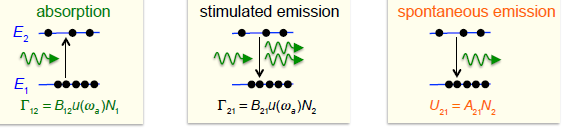
\includegraphics[scale=0.45]{ch1/image11.png}
	\captionof{figure}{ }
\end{center}
Dans le référentiel du centre de masse
\begin{equation}
v_{CM}=\frac{m_1}{m_1+m_2}v_{1i},\qquad\qquad\qquad v'=v-v_{CM}
\end{equation}
On en tire
\begin{equation}
v'_{1i}=v_{1i}-v_{CM}=\frac{m_2}{m_1+m_2}v_{1i}
\end{equation}
Comme nous avons une collision élastique dans le repère du centre de masse, seule la direction
est modifiée (et donc $v_{1f}'=v_{1i}'$)
\begin{equation}
v'_{1f}=\frac{m_2}{m_1+m_2}v_{1i}
\end{equation}

	\begin{wrapfigure}[8]{r}{5.5cm}
	\vspace{-5mm}
	\includegraphics[scale=0.65]{ch1/image12.png}
	\captionof{figure}{ }
	\end{wrapfigure}

L'angle maximal $\theta_{max}$ est obtenu lorsqu'un angle droit est formé au niveau de la
circonférence du cercle. On choisit alors $v_{1f}'$ ($v_{CM}$) étant fixé de sorte à avoir
$\theta_{max}$. Après un peu de trigonométrie
\begin{equation}
\sin{\theta_{max}}=\frac{v'_{1f}}{v_{CM}}=\frac{m_2}{m_1}
\end{equation}
Si $m_2\geq m_1$, on trouve $\theta_{max}=\pi$. \\

En conclusion\\

\cadre{\begin{itemize}
\item[$\bullet$] Grandes déviations possibles ($\theta_{max}=\pi/2$) pour l'interaction $e^-/e^-$
\item[$\bullet$] Très grandes déviations possibles ($\theta_{max}=\pi$) pour l'interaction $e^-/$ion
\item[$\bullet$] Petites déviations pour l'interaction ion/$e^-$
\item[$\bullet$] Grandes déviations possibles (dépendant de $m_1$ et $m_2$) pour l'interaction ion/
ion
\end{itemize}}

\subsection{Conclusions à propos de ces considérations de base}
\subsubsection{Pour les ions incidents}
De façon générale les pertes électroniques dominent (petits transfert d'énergie et petites déviations
angulaires) et les pertes nucléaires (collisions noyaux) sont rares (se produisent pour un 
faible nombre de projectives mais de grand transferts d'énergies sont possibles ainsi que de 
grandes déviations angulaires). Ils ont une \textit{trajectoire rectilignes accompagnées de 
pertes d'énergie faibles et continues}.

\subsubsection{Pour les électrons incidents}
Les pertes électroniques dominent (mais cette fois grands transferts d'énergie et grandes déviations
angulaires possibles). On retrouve aussi des pertes nucléaires (petits transferts d'énergie mais
très grandes déviations angulaires possibles (possibilité de rétro-diffusion). Ils ont une 
\textit{trajectoire courbée accompagnée de grandes pertes d'énergie}.






\chapter{Interaction des ions avec la matière}
	\begin{wrapfigure}[11]{l}{10.5cm}
	\vspace{-5mm}
	\includegraphics[scale=0.3]{ch2/image1.png}
	\captionof{figure}{ }
	\end{wrapfigure}
Ci-contre, à gauche, sont représenté les trajectoires de particules $\alpha$ d'une énergie
de 5.5 MeV. On observe que trois d'entre-elles sont rentrées en collisions avec les noyaux
(déviation angulaire plus importante). A droite, considérons un proton incident sur 
de l'aluminium, décrit par le modèle de Bohr. Ce modèle étant classique, il ne peut pas être
correct dans la zone relativiste. Lorsque la vitesse du projectile se rapproche de $v_0$, 
la vitesse de Bohr\footnote{On associe l'énergie à une certaine vitesse via l'énergie cinétique.}, 
on ne peut plus considérer que la particule est au repos, le modèle n'est dès lors plus 
valable\footnote{L'hypothèse de Bohr est telle que la particule cible est au repos.}

\section{Modèle semi-classique du pouvoir d'arrêt électronique}
Un rappel sur les oscillateurs classiques et l'approximation dipolaire est faite dans les
slides 5 à 12 : n'étant que des rappels/pré-requis, ils ne sont pas repris ici.

\subsection{Vitesses intermédiaires : $v_0\ll v \ll c$}
Dans le modèle semi-classique de \textsc{Bethe} (\textit{1930}), le noyau est traité 
classiquement et les électrons quantiquement, ils ne sont plus traités comme des oscillateurs
classiques. On s'intéresse ici au cas ou le modèle de Borh est correct. \\

Considérons un atome cible avec $Z_2$ électrons (masse $m$) et les états stationnaires $\ket j$ 
d'énergie $\epsilon_j$ où $j$ est un nombre quantique tel que $j=0$ dénote l'état fondamental. 
Les fréquences de résonance pour un atome dans son état initial sont données par
\begin{equation}
\hbar\omega_{j0}=\epsilon_j-\epsilon_0
\end{equation}
On dira que les électrons sont au repos durant l'interaction si $v\gg v_0$.
\\

Pour une énergie $Q$ perdue par l'ion incident, \textsc{Bethe} a posé
\begin{equation}
S=\sum_j\int Q d\sigma_Rf_{j0}(Q)
\end{equation}
où $\sigma_R$ est la section efficace de \textsc{Coulomb} pour un transfert d'énergie $Q$ 
(où $R$ pour \textsc{Rutherford}) et $f_{j0}$ sont les \textit{forces d'oscillateur généralisées}
qui incluent tous les effets quantiques pour la section efficace d'arrêt : ils décrivent les 
probabilités de transition entre les états pour une énergie transférée $Q$ donnée.\\

Afin de déterminer l'expression de $f_{j0}$, résolvons l'équation de Schrödinger dépendante du 
temps (celle-ci gouverne le mouvement électronique)
\begin{equation}
(H+V)\Psi(\overrightarrow{r},t)=i\hbar \frac{d\Psi(\overrightarrow{r},t)}{dt}
\end{equation}
où $H$ est l'hamiltonien d'un atome isolé de la cible, $\Psi(t)$ la fonction d'onde d'un état
lié et $V$ le potentiel décrivant l'interaction avec le projectile donné par
\begin{equation}
V(\overrightarrow{r},t)=\sum_{\nu=1}^{Z_2}\frac{-e_1e}{\overrightarrow{r}_\nu-\overrightarrow{R}(t)}
\end{equation}
où $\vec r = (\vec{r}_1,\dots \vec{r}_{Z_2})$ représente la trajectoire du projectile avec 
$\vec r_\nu$ l'opérateur position du $\nu^e$  électron et $\vec{R}=\vec{p}+\vec{v}t$. Développons
$\Psi(t)$ sur la base formée des états stationnaires
\begin{equation}
\Psi(\overrightarrow{r},t)=\sum_{j}c_j(t)e^{-i\epsilon_jt}|j\rangle
\end{equation}
où $\ket j$ sont les solutions de $H\ket j = \epsilon_j\ket j$. Dans le cadre de la méthode des
perturbations au premier ordre, on peut développer les coefficients $c_j$ en puissance du 
potentiel perturbatif $V$
\begin{equation}
c_j(t) = \delta_{j0} + c^{(1)}_j(t) + c^{(2)}_j(t) + \dots
\end{equation}
avec $\delta$ le symbole de Kronecker et

\begin{eqnarray}
c_j^{(1)}(t)=\frac{1}{i\hbar}\int_{-\infty}^{t}dt'e^{i\omega_{j0}t'}\langle j|V(\overrightarrow{r},t')|0\rangle\\
c_j^{(2)}(t)= \left(\frac{1}{i\hbar}\right)^2\sum_k\int_{-\infty}^{t}dt'e^{i\omega_{jk}t'}\langle j|V(\overrightarrow{r},t')|k\rangle
\times \int_{-\infty}^{t'}dt''e^{i\omega_{k0}t''}\langle k|V(\overrightarrow{r},t'')|0\rangle
\end{eqnarray}
et ainsi de suite mais ici nous ne nous intéressons que aux coefficients $c_j^{(1)}(\infty)$ car
seul le premier ordre nous intéresses. Ceux-ci représentent les amplitudes de transition. 
Substituons $c_j^{(1)}(\infty)$ dans l'expression explicite du potentiel, prenons-en la 
transformée de \textsc{Fourier} et intégrons sur $t'$
\begin{equation}
c_j^{(1)}(\infty)=\frac{-e_1e}{i\pi\hbar}\int \overrightarrow{dq}\frac{e^{-i\overrightarrow{q}.\overrightarrow{p}}}{q^2}F_{j0}(\overrightarrow{q})\delta(\omega_{j0}-\overrightarrow{q}.\overrightarrow{v})
\end{equation}
où $\DS F_{j0}(\overrightarrow{q})=\left\langle j\left| \sum_{\nu=1}^{Z_2}e^{i\overrightarrow{q}.\overrightarrow{r_\nu}}\right| 0\right\rangle$. Notons $Q=\frac{\hbar^2q^2}{2m}$. Par le 
\textsc{Postulat IV} de la mécanique quantique, les probabilités de transitions sont données 
par
\begin{equation}
P_j(p)=\left| \langle j| \Psi(\infty)\rangle\right|^2
\end{equation}
Ce qui donne dans le cadre de la méthode des perturbations au premier ordre
\begin{equation}
P_j(p)=\left| c_j^{(1)}(\infty)\right|^2
\end{equation}
Pour que $c_j^{(1)}(\infty) \neq 0$ pour $\omega_{j0} < q\nu$, il faut que (condition sur $Q$)
\begin{equation}
\omega_{j0}^2<q^2v^2 \Rightarrow 2mv^2Q>(\epsilon_j-\epsilon_0)^2
\end{equation}

\subsubsection{Approximation des collisions distantes - Approximation dipolaire}
Afin d'obtenir notre expression de $f_{j0}$, nous allons devoir utiliser une approximation. 
Considérons $c_j^{(1)}(\infty)$ à grand $p$ (\textit{collisions distantes}). Par l'approximation
dipolaire
\begin{equation}
e^{i\overrightarrow{q}.\overrightarrow{r}}\simeq 1+i\overrightarrow{q}.\overrightarrow{r}
\end{equation}
On obtient donc
\begin{equation}
F_{j0}(\overrightarrow{q})\simeq i\overrightarrow{q}\left\langle j\left| \sum_{\nu=1}^{Z_2}\overrightarrow{r_\nu}\right| 0\right\rangle
\end{equation}
En choisissant l'axe $x$ selon la vitesse du projectile et l'axe $y$ selon le paramètre 
d'impact, on voit apparaître des fonctions de \textsc{Bessel} modifiée $K_{0,1}$, d'ordre 0 et 1
\begin{equation}
c_j^{(1)}(\infty)=-\frac{2e_1e\omega_{j0}}{i\hbar v^2}\left\langle j\left| \sum_{\nu}^{Z_2}\overrightarrow{r}_\nu \right|0\right\rangle
 \times\left(iK_0\left(\frac{\omega_{j0}p}{v}\right),K_1\left(\frac{\omega_{j0}p}{v}\right),0\right)
\end{equation}
Les probabilités de transitions deviennent donc (données par $|c_j|^2$)
\begin{equation}
P_j(p)=-\frac{2e_1^2e^2Z_2}{mv^2p^2\hbar\omega_{j0}}f_{j0}
 \times\left\{\left[\frac{\omega_{j0}p}{v}K_0\left(\frac{\omega_{j0}p}{v}\right)\right]^2+\left[\frac{\omega_{j0}p}{v}K_1\left(\frac{\omega_{j0}p}{v}\right)\right]^2\right\}
\end{equation}
La grandeur $f_{j0}$ est appelée la \textbf{force d'oscillateur dipolaire} et a comme
expression
\begin{equation}
f_{j0}=\frac{2m}{3\hbar^2Z_2}(\epsilon_j-\epsilon_0)\left|\left\langle j\left|\sum_{\nu}^{Z_2}\overrightarrow{r}_\nu\right|0\right\rangle\right|^2
\end{equation}
Avec la règle de somme de \textsc{Thomas-Reiche-Kuhn} $\sum_j f_{j0}=1$.

\subsubsection{Comparaison modèle classique et semi-classique}
Maintenant que nous avons la probabilité d'une transition, il nous faut l'énergie moyenne. 
Considérons l'énergie transférée moyenne $T_{moy}$
\begin{equation}
T_{moy}(p)=\sum_jP_j(p)\hbar\omega_{j0}
\end{equation}
Comparons cette expression avec le résultat classique donné par 
\begin{equation}
T= \frac{2e_1^2e^2}{mv^2p^2}f_{dist}(p),\qquad\text{ où }\quad 
f_{dist}(p)=\left[\frac{\omega_{0}p}{v}K_0\left(\frac{\omega_{0}p}{v}\right)\right]^2+\left[\frac{\omega_{0}p}{v}K_1\left(\frac{\omega_{0}p}{v}\right)\right]^2
\end{equation}
Les expressions sont identiques à condition que
\begin{equation}
f_{dist}(p)=\sum_jf_{j0}\left[\frac{\omega_{j0}p}{v}K_0\left(\frac{\omega_{j0}p}{v}\right)\right]^2+\left[\frac{\omega_{j0}p}{v}K_1\left(\frac{\omega_{j0}p}{v}\right)\right]^2
\end{equation}
Pour généraliser les fonctions $f_{j0}$ que nous venons d'élaborer aux grandes valeurs de $Q$, 
\textsc{Bethe} a posé
\begin{equation}
f_{j0}(Q)=\frac{1}{Z_2}\frac{\epsilon_j-\epsilon_0}{Q}|F_{j0}(\overrightarrow{q})|^2
\end{equation}
Avec cette forme la, lorsque $Q$ est petit, on retrouve l'expression que nous venons de calculer
\begin{equation}
f_{j0}(Q)\big\vert_{Q\simeq 0}=f_{j0}
\end{equation}

\subsubsection{Pouvoir d'arrêt : formule de Bethe}
Il est nécessaire de faire la distinction entre les collisions distantes ou proche (via $p$), soit 
les collision avec une grande ou petite quantité de mouvement transférée (via $q$) ou encore 
les collisions avec une grande ou petite énergie transférée (via $Q$). Pour se faire, 
nous allons séparer l'intégrale suivante en deux parties par rapport à $Q_0$
\begin{equation}
S=\sum_j\int Q d\sigma_Rf_{j0}(Q)
\end{equation}
$\bullet$ Pour $Q<Q_0$, l'approximation dipolaire est valide ($Q_0$)
\begin{equation}
S_{dist}=\sum_jf_{j0}\int_{(\epsilon_j-\epsilon_0)^2/2mv^2}^{Q_0} Q d\sigma_R
\end{equation}

$\bullet$ Pour $Q>Q_0$, il faut déterminer la borne supérieure de l'intégrale. On considère que 
la masse d'un ion $m_1\gg m$, la masse d'un électron.
\begin{equation}
T_{max} = \gamma E = \frac{4m_1m}{(m_1+m)^2}\frac{m_v^2}{2} \approx 2mv^2
\end{equation}
où nous avons négliger $m$ par rapport à $m_1$. On trouve alors la section efficace 
d'arrêt suivante
\begin{equation}
S_{proche}=\int_{Q_0}^{2mv^2} Q d\sigma_R\sum_jf_{j0}(Q)
\end{equation}
\textsc{Bethe} a démontré que
\begin{equation}
\sum_jf_{j0}(Q)=1
\end{equation}
Nous avons alors
\begin{equation}
S_{proche}=\int_{Q_0}^{2mv^2} Q d\sigma_R\equiv \sum_jf_{j0}\int_{Q_0}^{2mv^2} Q d\sigma_R
\end{equation}
En sommant les collisions proches et distantes, on trouve finalement
\begin{equation}
S=S_{proche}+S_{dist}= \sum_jf_{j0}\int_{(\epsilon_j-\epsilon_0)/2mv^2}^{2mv^2} Q d\sigma_R
\end{equation}
En considérant l'expression explicite $d\sigma_R= 2\pi \frac{e_1^2e_2^2}{m_2v^2}\frac{dQ}{Q^2}$, 
on obtient
\begin{equation}
S=\frac{4\pi e_1^2e^2}{mv^2}Z_2\sum_jf_{j0}\ln{\frac{2mv^2}{\epsilon_j-\epsilon_0}}
\end{equation}
La formule du pouvoir d'arrêt de \textsc{Bethe} se note généralement\\

\cadre{\begin{equation}
S_{e}=\frac{4\pi e_1^2e^2}{mv^2}Z_2\ln{\frac{2mv^2}{I}}
\end{equation}
où $I$ est définie comme l'énergie moyenne d'excitation telle que $\ln I=\sum_j f_{j0}\ln{
(\epsilon_j-\epsilon_0)}$. Ceci n'est valable que \textbf{si} $m_1\gg m, v\gg v_0 \to mv^2 \gg
 \hbar \omega_0$.}\ \\
 
On peut facilement comparer le modèle de \textsc{Bethe} à celui de \textsc{Bohr} via 
\begin{equation}
S_e=\frac{4\pi Z_2 e_1^2e^2}{mv^2}L_e
\end{equation}
où 
\begin{equation}
L_e=\ln\frac{Cmv^3}{|e_1e|\omega_0}
\end{equation}
pour le \textsc{Bohr} et 
\begin{equation}
L_e=\ln{\frac{2mv^2}{I}}
\end{equation}
pour \textsc{Bethe}.

\subsubsection{Dépendances principales du pouvoir d'arrêt}
Le pouvoir d'arrêt se compose lui-même de trois dépendances\ \\

\retenir{\begin{equation}
-\left( \frac{dE}{dx}\right)_{elec}=NS_{e}=\frac{4\pi e_1^2e^2}{mv^2}NZ_2\ln{\frac{2mv^2}{I}}
\end{equation}}\ \\

Les dépendances sont les suivantes
\begin{enumerate}
\item $\frac{4\pi e_1^2e^2}{mv^2}\Rightarrow{\mbox{D\'ependance principale dans la vitesse}}$, plus la vitesse augmente, plus le pouvoir d'arrêt diminue.
\item $NZ_2\Rightarrow{\mbox{D\'ependance principale dans le mat\'eriau}}$, plus il est grand, plus le pouvoir augmente.
\item $\ln{\frac{2mv^2}{I}}\Rightarrow{\mbox{D\'ependance faible dans la vitesse et dans le mat\'eriau}}$
\end{enumerate}

	\subsubsection{Énergies moyenne d'excitation}
	\begin{wrapfigure}[7]{r}{6.5cm}
	\vspace{-5mm}
	\includegraphics[scale=0.5]{ch2/image2.png}
	\captionof{figure}{ }
	\end{wrapfigure}
	

L'énergie moyenne d'excitation $I$ ne dépend \textbf{que} du matériau et \textbf{pas} du 
projectile. Il est possible de le calculer mais tout le monde s'en fiche car on peut l'obtenir
expérimentalement\footnote{De plus, comme il intervient dans $\log S$ il n'est pas nécessaire
de connaître sa valeur avec précision} via des formules empiriques. Celui-ci varie approximativement
linéairement (les irrégularités sont dues à la structure en couches de l'atome) avec $Z$ :
\textit{modèle de l'atome de Thomas-Fermi} où les électrons atomiques forment un gaz.

\newpage
\subsection{Grandes vitesses - Équation de \textsc{Bethe-Bloch} : $v_0<v\approx c$}
\textsc{Bloch} a apporté de nombreuses corrections à l'équation de \textsc{Bethe} pour 
former l'équation de \textsc{Bethe-Block}\\

\cadre{\begin{equation}
S_e = \dfrac{4\pi r_e^2mc^2}{\beta^2}Zz^2L(\beta)
\end{equation}
où $\DS L(\beta)= L_0(\beta) = \frac{1}{2}\ln\left(\frac{2mc^2\beta^2W_m}{1-\beta^2}\right)
-\beta^2-\ln I-\frac{C}{Z}-\frac{\delta}{2}$.}\ \\

Il s'agit en réalité de la même équation mais notée différemment, toute la différence se 
trouve dans le \textit{stopping number} $L$ qui contient donc les termes correctifs. 
Intéressons-nous à ceux-ci
\begin{itemize}
\item[$\bullet$] \textit{Corrections dues aux collisions}\ \\
$W_m$ donne l'énergie maximale transférée en une collision à un électron
libre\footnote{Il s'agit d'une expression relativiste non-approchée}
\begin{equation}
W_m=\frac{2mc^2\beta^2}{1-\beta^2}\left[1+\frac{2m}{m_1(1-\beta^2)^{1/2}}+\left(\frac{m}{m_1}\right)^2\right]^{-1}
\end{equation}
Pour $m_1\gg m$, on retrouve bien $2m\gamma_1^2v^2$.
\item[$\bullet$] \textit{Corrections relativistes}\ \\
Si $v\approx c$, il faut apporter des corrections relativistes. Lorsque l'on travaille avec
des vitesses relativistes, il faut considérer des électrons de plus en plus lointain ce qui, 
forcément, augmente le pouvoir d'arrêt. En effet, $p_{max} \propto \gamma_1v/\omega_0$ ce qui
montre que le paramètre d'impact augmente lorsque la vitesse fait de même. Le calcul relativiste
classique du champ donne
\begin{equation}
\overrightarrow{E}(\omega)=-\frac{e_1\omega}{\pi \gamma_1v^2}\left(\frac{i}{\gamma_1}K_0\left(\frac{\omega_{j0}p}{\gamma_1v}\right),K_1\left(\frac{\omega_{j0}p}{\gamma_1v}\right),0\right)
\end{equation}
On y voit apparaître des $\gamma_1$ et $f(p)$ se voit modifiée par ce fameux terme
\begin{equation}
f_{dist}(p)=\frac{1}{\gamma_1^2}\left[\frac{\omega_{0}p}{\gamma_1v}K_0\left(\frac{\omega_{0}p}{\gamma_1v}\right)\right]^2+\left[\frac{\omega_{0}p}{\gamma_1v}K_1\left(\frac{\omega_{0}p}{\gamma_1v}\right)\right]^2
\end{equation}
La composante principale en la vitesse se voit modifiée
\begin{equation}
\frac{4\pi e_1^2e^2}{mv^2}\Rightarrow \frac{4\pi e_1^2e^2}{m\gamma_1^2v^2}=\frac{4\pi e_1^2e^2}{mv^2}(1-\beta^2)
\end{equation}
où le $(1-\beta^2)$ apparaissant permet de comprendre le terme correspondant dans la formule de 
\textsc{Bethe-Bloch}, il va être possible de lui donner un sens physique. Sachant que la quantité 
de mouvement de la particule incidente devient $m\gamma_1v$, on en tire
\begin{equation}
T_{max}=2m\gamma_1^2v^2
\end{equation}
La composant logarithmique se modifie selon
\begin{equation}
\ln{\frac{2mv^2}{I}}\Rightarrow \ln{\frac{2m\gamma_1^2v^2}{I}}=\ln{\frac{2mv^2}{I(1-\beta^2)}}
\end{equation}
La combinaison de toutes ces relations implique donc que le pouvoir d'arrêt augmente lorsque 
la vitesse augmente, ce qui est la conséquence du traitement relativiste. 
\end{itemize}

\newpage

\begin{itemize}
\item[$\bullet$] \textit{Correction de densité}\ \\
Le terme correspondant à ces corrections est le $-\delta/2$. La formule de \textsc{Bethe} est 
valable pour un gaz de faible densité (atomes isolés) mais pour un solide il faut tenir compte
des effets collectifs d'un grand nombres d'atomes : on peut utiliser le modèle de Fermi. Une 
particule chargée incidente va polariser le milieu. Le champ électrique induit va alors donner un
moment dipolaire électrique aux atomes et il en résultera un champ électrique opposé à celui 
produit par la particule chargée. Le champ électrique sera donc réduit via l'écrantage des dipôles.\\

A cause de cette diminution du champ (à cause de la polarisation), les atomes lointains ont un 
effet plus faible. L'effet de densité apparaît surtout aux grandes vitesses, en même temps que les 
effets relativiste (ils vont se "compenser"). S'il n'est signifiant qu'aux énergies élevées c'est 
à cause du facteur $\gamma_1$ présent dans $p_{max}$ qui augmente l'erreur commise en ignorant la
polarisation du milieu : si $v$ augmente, $p_{max}$ augmente et donc $\delta/2$ augmente causant une
diminution de $S$.

\begin{center}
	\includegraphics[scale=0.5]{ch2/image3.png}
	\captionof{figure}{L'effet relativiste et de densité vont se stabiliser de sorte que le 
	pouvoir d'arrêt devient constant. On parle alors de \textit{plateau de Fermi}, constant à
	grande vitesse.}
\end{center}

On peut écrire la correction de densité
\begin{equation}
\frac{\delta}{2}=\ln{\frac{\hbar\omega_p}{I}}+\ln{\gamma_1\beta}-\frac{1}{2}
\end{equation}
avec $\omega_p=\sqrt\frac{ne^2}{\epsilon_0m}$ la \textit{pulsation plasma}, mais ceci est plus
informatif.

\item[$\bullet$] \textit{Correction shell} ("en couches")\ \\
Il s'agit du terme $-C/Z$. Nos deux formules sont basées sur l'hypothèse que $v\gg v_0$ (permet
de calculer $I$ moyen). Lorsque que n'est plus le cas, on ne peut plus considérer que tous les
électrons ont la même énergie de liaison. Le problème est que certains électrons sont plus liés 
que d'autres. Comme ils seront plus durs à arracher, leur contribution au pouvoir d'arrêt va 
diminuer et il ne faudra plus les considérer. On ajoute ainsi un terme de correction "moyen" qui
réduit $S$ de maximum 6\% qui ne dépend que de la vitesse et du matériau considéré, peu importe 
les couches. Il existe deux méthodes pour calculer $C/Z$
	\begin{enumerate}
	\item Une basées sur les fonctions d'ondes hydrogénoïdes (HWF)\footnote{Un électron interne ne
	 peut
	 pas être représenté par une fonction d'onde de la sorte mais comme la rigueur absolue n'est 
	 pas possible en s'en contentera car \textit{au moins} on a un résultat, bien que moins 
	 rigoureux.}
	\item Une basée sur l'approximation en densité locale (LDA)
	\end{enumerate}
	
%\begin{center}
\hspace{-1cm}	\includegraphics[scale=0.4]{ch2/image4.png}
	\captionof{figure}{A gauche la comparaison théorie/expérience (relativement bonne et comme la
	correction est logarithmique on s'en contentera), au centre le calcul par la méthode LDA et à
	droite selon HWF. L'écart entre les méthodes est plus grand pour des $Z$ élevés mais 
	les deux sont globalement assez bonnes.}
%\end{center}
\end{itemize} \ \\

Il est possible d'aller encore plus loin et de considérer des corrections au-delà de l'approximation
de \textsc{Born} au premier ordre.  On va considérer des vitesses toujours plus grande que $v_0$ mais
très proche de celle-ci de sorte que l'approximation de Born n'est plus valable\footnote{Il faut 
en effet que $v\gg v_0$ pour que $L_0$ soit valable}.Il faut rajouter des termes correctifs à 
$L_0$ qui apparaissent lors d'un développement de $L$ en puissance de $z$\ \\

\cadre{\begin{equation}
L(\beta) =  L_0(\beta) + zL_1(\beta) + z^2L_2(\beta)
\end{equation}}\ \\

Passons à nouveau en revue les différentes corrections
\begin{itemize}
\item[$\bullet$] \textit{Correction de Barkas-Andersen}\ \\
Il s'agit du terme $zL_1(\beta)$. Il s'agit d'une proportionnalité à une puissance impaire de la 
charge. Si la charge est positive, cela attire le nuage d'électrons et il y aura plus d'interactions :
augmentation du pouvoir d'arrêt. Si la charge est négative, les électrons sont repoussés et le 
pouvoir d'arrêt diminue. $S$ diffère donc entre les particules et antiparticules.
\begin{center}
	\includegraphics[scale=0.5]{ch2/image5.png}
	\captionof{figure}{Protons et antiprotons incidents sur une cible de silicium : le pouvoir 
	d'arrêt est plus important pour les protons que pour des antiprotons.}
\end{center}
\item[$\bullet$] \textit{Correction de Bloch}\ \\
Il s'agit du terme $z^2L_2(\beta)$, une correction pas très importante que l'on évalue généralement
avec l'évaluation de \textsc{Bichsel}
\begin{equation}
z^2L_2(y) = -y^2[1.202-y^2(1.042-0.855y^2+0.343y^4)]
\end{equation}
où $y=z\alpha/\beta$ avec $\alpha = 1/137$ le constante de structure fine.
\end{itemize}

\newpage
	\begin{wrapfigure}[11]{r}{9cm}
%	\vspace{-5mm}
	\includegraphics[scale=0.4]{ch2/image6.png}
	\captionof{figure}{ }
	\end{wrapfigure}
Évaluons maintenant les effets des différentes corrections. Le graphique ci-contre (à gauche) 
concerne des protons incidents sur une cible d'aluminium. On peut y voir que la correction de
\textsc{Bloch} (en bas à gauche) est vraiment très faible. A droite est représenté la correction
relative pour des protons incidents sur une cible d'or ($L_1$ concerne \textsc{Barkas} et $L_2$
\textsc{Bloch}).


\subsection{Petites vitesses}
Lorsque $v \lesssim v_0$, on ne peut plus appliquer la méthode des perturbations et il faut 
commencer à prendre en compte les captures électroniques par l'ion indicent (l'ion va si
lentement qu'il peut capturer un (ou plusieurs) électron) modifiant la charge $z^*$ de 
celui-ci. Par la théorie de \textsc{Thomas-Fermi}
\begin{equation}
z^*=z\left(1-e^{-v/(z^{2/3}v_0)}\right)
\end{equation}
Une technique consiste à considérer un état de charge moyen même si ce n'est pas vrai en tout 
point.


\section{Pouvoir d'arrêt nucléaire (faibles vitesses)}
Les effets étant tellement négligeable que nous ne rentrerons pas dans les détails ici. Comme
vu au premier chapitre, les collisions nucléaire pour des ions incidents sont rares et contribuent
peu au pouvoir d'arrêt total. Elle se produise presque exclusivement pour des ions incidents de 
faible vitesse et même alors leur contribution est faible. Cependant, elle peuvent avoir des effets
à postériori et causer des dégâts radiatifs.\\

	\begin{wrapfigure}[12]{r}{5.6cm}
	\vspace{-11mm}
	\includegraphics[scale=0.34]{ch2/image7.png}
	\captionof{figure}{ }
	\end{wrapfigure}
Plaçons-nous dans le système du centre de masses pour observer la diffusion par un angle 
$\theta$ due à un potentiel central $V(r)$. Reprenons la formule générale pour la section efficace
d'arrêt 
\begin{equation}
S_n = \int Td\sigma = \int T 2\pi p dp = 2\pi\gamma E\int \sin^2(\theta/2)pdp
\end{equation}
où $\gamma = \frac{4m_1m_2}{(m_1+m_2)^2}$. Pour le calculer, il est nécessaire de connaître $\theta$
ce qui peut se faire avec le schéma avec une particule incidente et cible représenté ci-contre.\\

Pour évaluer $\theta$, on utilise l'équation de la variation angulaire en coordonnée sphérique tout
en introduisant le potentiel. 

\begin{eqnarray*}
\frac{m_0}{2}\left[ \left( \frac{dr}{dt}\right)^2+r^2\left( \frac{d\varphi}{dt}\right)^{2}\right]+V(r)=\frac{m_0}{2}v^2\equiv E_r\\
m_0r^2\frac{d\varphi}{dt}=-m_0pv
\end{eqnarray*}
On en tire
\begin{equation}
\theta=\pi-2\int_{r_{m}}^\infty dr \frac{p}{r^2}\left( 1-\frac{V(r)}{E_r}-\frac{p^2}{r^2}\right)^{-1/2}
\end{equation}


Il faut maintenant spécifier le potentiel. Le plus logique serait d'utiliser celui de \textsc{Coulomb}
mais sa variation en $1/r$ cause une divergence du paramètre d'impact à cause de la portée infinie. 
Comme il y a toujours interaction, on va préférer considérer un effet d'écrantage par les électrons
atomiques qui diminue la portée du potentiel. Pour se faire, on va simplement introduire une 
exponentielle décroissante $\exp(-r/r_s)$.\\

Pour un modèle plus précis, on peut insérer une fonction $F_s(r/r_s)$. Le potentiel d'interaction 
devient alors
\begin{equation}
V(r)=\frac{z_1Z_2e^2}{r}F_s(\frac{r}{r_s})
\end{equation}
Il s'agit de la \textit{fonction d'écrantage universelle}, obtenue par ajustement aux résultats 
expérimentaux.\\

	\begin{wrapfigure}[12]{r}{5.6cm}
	\vspace{-11mm}
	\includegraphics[scale=0.34]{ch2/image8.png}
	\captionof{figure}{ }
	\end{wrapfigure}
Mettons maintenant ces effets ensemble en considérant des protons incidents sur une cible 
d'aluminium comme représenté ci-contre. Nous avons $S = S_{elec} + S_{nucl} \approx S_{elec} 
= S_{coll}$. On voit que l'effet du pouvoir d'arrêt nucléaire est très faible, on retrouve
le plateau de Fermi à grande vitesse et une pente ou la formule de \textsc{Bohr} est valable.


\section{Pouvoir d'arrêt massique électronique et influence de la phase}
Par définition, le pouvoir d'arrêt massique d'un matériau est le rapport du pouvoir d'arrêt 
linéique et de lamasse volumique $\rho$ de ce matériau (unités usuelle : MeV.cm$^2$.g$^{-1}$. 
\begin{equation}
\frac{NS(E)}{\rho}=-\frac{1}{\rho}\frac{dE}{dx}
\end{equation}
Comme $\rho = M_AN/N_A$ où $M_A=AM_u$, en divisant des deux côtés par cette même quantité on 
trouve\\

\cadre{\begin{equation}
-\dfrac{1}{\rho}\dfrac{dE_{elec}}{dx} = 4\pi r_e^2mc^2\frac{N_A}{M_u}\dfrac{Z}{A}\dfrac{z^2}{\beta^2}
L(\beta)
\end{equation}}\ \\

Passons en revue les quatre facteurs du pouvoir d'arrêt massique électronique
\begin{enumerate}
\item Le facteur constant $4\pi r_e^2mc^2N_A/M_u = 0.307$ MeV.cm$^2$.g$^{-1}$ qui donne l'ordre
de grandeur de ce pouvoir
\item Le facteur $Z/A$ compris entre 0.4 et 0.5 pour tout les isotopes stable (sauf $H$). Comme
c'est le terme principal de dépendance du matériau et que celui-ci est $\pm$ constant la dépendance
du matériau est faible : c'est l'intérêt de cette formule
\item Le facteur $\beta^{-2}$ est une fonction monotone décroissante de la vitesse de l'ion qui
tend vers 1 pour les grandes énergies. Ce-dernier explique la diminution du pouvoir d'arrêt 
avec l'énergie. 
\item Le nombre d'arrêt $L(\beta)$ est une fonction monotone croissante (lente) de la vitesse 
et de $Z$.
\end{enumerate}

\subsection*{Influence de la phase}
Aux grandes énergies, la correction de densité influe impliquant une grande correction de phase 
dans les solides et faible dans les gaz. Aux faibles énergies il faut tenir compte de l'influence
des liaisons chimiques et intermoléculaires ce qui se traduit par une modification de la
valeur de $I$.

\section{Parcours et courbe de Bragg} 
\subsection{Parcours}
Lorsque les particules \textbf{chargées} perdent leur énergie dans la matière, elles parcourent une
certaine distance dans la matière mais celle-ci peut être variable a cause des pertes d'énergies 
et des déviations aléatoires (\textit{starggling}). Il faut alors définir plusieurs parcours
\begin{itemize}
\item[$\bullet$] Le parcours $R$ d'une particule chargée d'énergie $E$ dans un milieu et 
la valeur moyenne $\langle l \rangle$ de la longueur $m$ de sa trajectoire suivie jusqu'à son 
arrêt (en négligeant le mouvement thermique)
\item[$\bullet$] Le parcours projeté $R_p$ d'une particule chargée d'énergie $E$ dans un milieu. 
Celui-ci correspond à la valeur moyenne de sa profondeur de pénétration $\langle d \rangle$ dans la
direction initiale de la particule.
\end{itemize}
A cause du caractère sinueux des trajectoires, $R_r<R$. On défini alors le \textbf{facteur de détour}
$R_p/R_{CSDA} < 1$.\\

Dans l'approximation $CSDA$
\begin{equation}
R_{CSDA}=\int^{E}_{0}\frac{dE'}{NS(E')}
\end{equation}
En remplaçant $S$ par l'expression de \textsc{Bethe} (non-relativiste, avec $dE=Mv$d$v$)
\begin{equation}
R_{CSDA}\propto \int^{v}_{0}\frac{v^3dv}{L(v)}
\end{equation}
En négligeant la dépendance en la vitesse du nombre d'arrêt 
\begin{equation}
R_{CSDA}\propto v^4\propto E^2
\end{equation}
En réalité, l'équation de \textsc{Bethe} (ou \textsc{Bethe-Bloch}) n'est pas valable à faibles
vitesses et il faut nécessairement passer par de faibles vitesses pour s'arrêter. On utilisera 
alors la formule empirique suivante
\begin{equation}
\rho R_{CSDA}=\frac{E^{1.77}}{415}+\frac{1}{670}
\end{equation}

\subsubsection{Considérations sur le parcours}
Reprenons l'approximation $NS(E)\propto 1/E$. Soit une particule incidente de masse $M_i$ et de
charge $z_i$
\begin{equation}
NS(E)=-\frac{dE}{dx} \Rightarrow -\frac{M_i}{z_i^2}\frac{dv^2}{dx}\propto \frac{1}{v^2}
\end{equation}
Pour deux particules incidentes $(M_1,z_1)$ et $(M_2, z_2)$ de même vitesse initiale
\begin{equation}
\frac{R_{CSDA}^1}{R_{CSDA}^2}=\frac{M_1z_2^2}{M_2z_1^2}
\end{equation}
Il s'agit d'une petite formule utile pour estimer l'ordre de grandeur qui nous informe que le range
pour des protons et des $\alpha$ de même vitesse est similaire.


\subsection{Courbes de Bragg}
Soit un milieu semi-infini et un faisceau parallèles de particules chargées identiques et de même
énergie : toutes les particules vont forcément s'arrêter, après une distance $R_{CSDA}$. La 
courbe de \textsc{Bragg} donne la \textbf{dose} (énergie moyenne déposée par unité de masse de la
cible) déposée par la particule chargée en fonction de la profondeur. \\

A une profondeur $x$, la particule doit encore parcourir $d=R_{CSDA}-x$. Comme l'énergie déposée
$D \propto S \propto 1/v^2$, cela implique que $R_{CSDA}\propto v^4$. Dès lors
\begin{equation}
D\propto \frac{1}{\sqrt d}=\frac{1}{\sqrt{R_{CSDA}-x}}
\end{equation}

	\begin{wrapfigure}[12]{r}{8.5cm}
	\vspace{-7mm}
	\includegraphics[scale=0.5]{ch2/image9.png}
	\captionof{figure}{Protons de 700 MeV dans de l'eau}
	\end{wrapfigure}
Ceci a des applications en protonthérapie (ou hadronthérapie). Lorsque l'on a une tumeur, il faut
la soumettre à un rayonnement pour l'éliminer. On pourrait envoyer des électrons, mais entre la 
tumeur et la peau il y a pas mal de choses qu'il ne vaut mieux pas endommager et le problème est que 
les électrons vont déposer pas mal d'énergie entre les deux. Avec la protonthérapie, la zone dans 
laquelle il ne faut pas déposer l'énergie sera faible et le maximum d'énergie sera déposé la ou 
la tumeur se situe.\\

\subsection*{Interactions nucléaires fortes}
	\begin{wrapfigure}[5]{l}{3cm}
	\vspace{-7mm}
	\includegraphics[scale=1.5]{ch2/image10.png}
%M	\captionof{figure}{ }
	\end{wrapfigure}
Lorsqu'un ion s'approche très près d'un noyau, une interaction nucléaire forte est possible et le
noyau peut être brisé. Par exemple, en fragmentant le plomb on aura un excès de neutron. Ce 
processus de production de neutrons est nomme \textit{spallation}. Le projet \textit{Myrrha} se
base la dessus. L'idée est de faire un réacteur avec un accélérateur en envoyant des protons sur
du Pb pour produire des neutrons et après se trouve un réacteur classique : pour l'arrêter, il suffit
de couper l'accélérateur.
%\chapter{Bruits et parasites}
Introduisons la notion de  bruit et parasite:
\begin{description}
	\item[Bruit] au sens strict (encore appelé "bruit de fond") est un signal à variation aléatoire d'origine \emph{interne} au dispositif étudié. Il est possible de le définir, de prévoir son niveau plancher à l'aide du dimensionnement
	\item[Parasites] signaux perturbateurs d'origine \emph{externe} au dispositif
\end{description}
Ces 2 phénomènes se présentent sous forme de signal analogique venant s'additionner au signal utile, entraînant ainsi sa dégradation. Une fois le signal utile perturbé, pas de marche arrière, d'où l'importance des ces concepts lors du dimensionnement.
\begin{table}[H]
	\centering
	\begin{tabular}{lcr}
		& \textbf{bruit} & \textbf{parasite} \\ \hline
		origine & interne & externe \\
		distribution & aléatoire & variable \\
		bande passante & "\(\infty\)" & limitée \\
		amplitude & faible & variable \\
		& "plancher" & arbitrairement bas \\
		modélisation & "facile" & difficile \\
		contre-mesures & conception & conception/remédiation \\ \hline
 	\end{tabular}
	\caption{Critères de distinction}
\end{table}
On remarque que:
\begin{itemize}
	\item contrairement au bruit qui possède généralement une amplitude plancher, calculable théoriquement, il est théoriquement impossible de réduire les parasites à un niveau arbitrairement bas.
	\item La modélisation des effets du bruit dans un système est, dans le principe, simple. Au contraire, la modélisation des parasites est nettement plus difficile car ceux-ci sont constitués de plusieurs signaux plus déterministes dont il faut connaître les couplages avec le système étudié.
\end{itemize}
L'introduction des ces phénomènes relève tout l'intérêt des signaux numérique (au lieu d'analogique). En effet, alors qu'un signal analogique dégradé ne peut être restauré, il est possible généralement de restaurer un signal numérique dégradé.\\
Un signal numérique n'est rien d'autre qu'un signal analogique dont certains niveaux représentent des valeurs discrètes portant une information (paliers, ex. 0=vrai, 1=faux) et dont chaque niveau peut varier dans certaines limite \(\rightarrow\) marges de bruit.\\

Ainsi, si l'impact des bruits et parasites est inférieur à cette marge de bruit définie par la conception, il est possible de restaurer le signal numérique utile. Les signaux numériques présentent donc une meilleure robustesse face aux perturbations. Il sera néanmoins toujours nécessaire de limiter les perturbations (car marges de bruit limitées).
\section{Le bruit de fond}
\subsection{Introduction}
Le bruit de fond possède plusieurs caractéristiques:
\begin{itemize}
	\item fluctuation aléatoire fondamentale due à la nature elle-même du dispositif
	\item limite ultime de la résolution du dispositif (contrairement aux parasites)
	\item fondamentalement inévitable (jamais nul) mais son influence sur la chaîne peut être minimisée
	\item origine générale en électronique: fluctuations de la densité des porteurs de charges (porteurs de charges = \(e^-\) et trous, fonction de la température)
	\item observable sur une tension et/ou un courant
\end{itemize}
Il existe plusieurs type de bruit, comme le bruit de type gaussien (c-à-d qui suit une loi normale de moyenne et variance données \(N(\mu,\sigma)\), \autoref{fig:densiteprobagauss})

\begin{figure}[H] 
	\centering 
\pgfmathdeclarefunction{gauss}{2}{%
	\pgfmathparse{1/(#2*sqrt(2*pi))*exp(-((x-#1)^2)/(2*#2^2))}%
}
	\begin{tikzpicture}[
	scale=0.6,
	every pin edge/.style={<-},
	every pin/.style={fill=yellow!50,rectangle,rounded corners=3pt,font=\small}]
	\begin{axis}[every axis plot post/.append style={
		mark=none,domain=-3:3,samples=30,smooth},
	clip=false,
	axis y line=none,
	axis x line*=bottom,
	ymin=0,
	xtick=\empty,
	]
	\addplot {gauss(0,0.5)};
	\addplot {gauss(0,1)};
	\draw[dashed]  (axis description cs:0.5,0) node[below] {\(\mu\)} -- (axis description cs:0.5,0.92) ;
	\end{axis}
	\end{tikzpicture}
\caption{Bruit de type gaussien: densité de probabilité}
\label{fig:densiteprobagauss}
\end{figure}
Valeur maximale du bruit ? Prenons un bruit de valeur efficace \(\SI{1}{\volt}\) (\autoref{fig:tensionbruitmax}). Il est tout à fait possible qu'au bout de \(\SI{100}{\second}\) on ait un bruit 10 fois plus grand. C'est aléatoire, mais sa puissance rms est constante.
\begin{figure}[H] 
	\centering 
	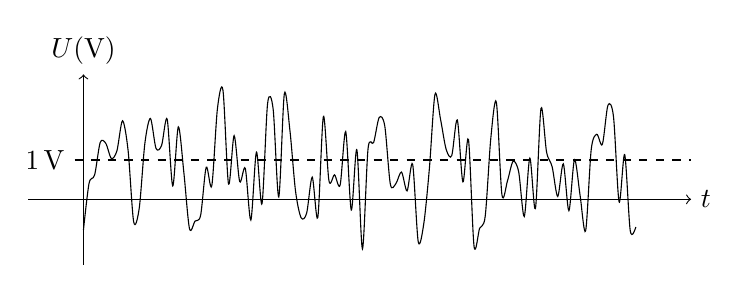
\begin{tikzpicture}[samples=100, domain=0:5*360]
	\begin{axis}[
	width=10cm, height=4cm,
	enlarge x limits=true,
	xtick=\empty,
	ytick=\empty,
	axis line style={->},
	axis lines*=middle,
	xlabel=\(t\),
	ylabel=\(U(\si{\volt})\),
	every axis x label/.style={
		at={(ticklabel* cs:1)},
		anchor=west,
	},
	every axis y label/.style={
		at={(ticklabel* cs:1)},
		anchor=south,
	},]
	\addplot [no markers, smooth] {sin(x)*sin(x)+rand};
	\draw[dashed] (axis description cs:0.07,0.55) node[left] {\SI{1}{\volt}} -- (axis description cs:1,0.55) ;
		\end{axis}
	\end{tikzpicture}
	\caption{Bruit de type gaussien: tension} 
	\label{fig:tensionbruitmax}
\end{figure}

\paragraph{Remarque:} la "valeur efficace" est une puissance mesurée, ce n'est pas le max
\subsection{Caractérisation mathématique}
\subsubsection{Définition de base}
Mathématiquement, le bruit est caractérisé par un \emph{signal temporel} (f.e.m) \(E_b(t)\) avec les propriétés suivantes:
\begin{itemize}
	\item {\makebox[8cm]{fluctuation aléatoire \(\Rightarrow\) moyenne nulle\hfill} \(\overline{E_b(t)}=0\)}
	\item {\makebox[8cm]{valeur quadratique moyenne non nulle\hfill} \(\overline{E_b^2(t)} \neq 0\)}
	\item {\makebox[8cm]{valeur efficace ("rms" = root mean square)\hfill} \(E_b=\sqrt{\overline{E_b^2(t)}}\)}
	\item {\makebox[8cm]{rapport signal/bruit SNR [dB]\hfill} \(SNR=10\log\left(\overline{E^2_s(t)}/\overline{E_b^2(t)}\right)\)}
\end{itemize}
\subsubsection{Variation en fréquence}
À ces propriétés s'ajoutent:\begin{itemize}
	\item La valeur efficace dépend de la fréquence \(\Rightarrow\) \emph{densité spectrale} de bruit \[e_b(f)=\sqrt{\left.\frac{d\overline{E_b^2}}{df}\right|_f}\quad [\si[per-mode=symbol]{\volt\per\sqrt{\hertz}}]\]
	\item La couleur du bruit:
	\begin{itemize}
		\item bruit blanc: densité spectrale constante en fréquence (uniformément réparti en fréquence, \autoref{fig:bruitblanc})
		\item bruit rose: densité spectrale plus forte pour les basses fréquences (descente linéaire, \autoref{fig:bruitrose})
	\end{itemize}
\end{itemize}
\begin{figure}[H]
	\centering
	\subfigure[Bruit blanc]{\label{fig:bruitblanc}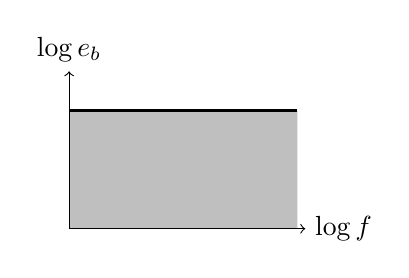
\begin{tikzpicture}
		\fill [gray!50, domain=0:2.9, variable=\x]
		(0, 0)
		-- plot ({\x}, {1.5})
		-- (2.9, 0)
		-- cycle;
		\draw[->] (0,0) -- (0,2) node[above]{\(\log e_b\)};
		\draw[->] (0,0) -- (3,0) node[right]{\(\log f\)};
		\draw[very thick] (0,1.5) -- (2.9,1.5);
		\end{tikzpicture}}
	\subfigure[Bruit rose]{\label{fig:bruitrose}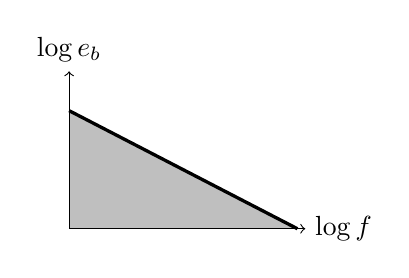
\begin{tikzpicture}
		\fill [gray!50, domain=0:2.9, variable=\x]
		(0, 0)
		-- plot ({\x}, {1.5-\x*0.51})
		-- (2.9, 0)
		-- cycle;
		\draw[->] (0,0) -- (0,2) node[above]{\(\log e_b\)};
		\draw[->] (0,0) -- (3,0) node[right]{\(\log f\)};
		\draw[very thick] (0,1.5) -- (2.9,0);
		\end{tikzpicture}}
	\caption{Répartition en fréquence de la densité spectrale de bruit}
\end{figure}
\subsubsection{Sommation de bruits divers}
Dans l'hypothèse où il n'y a pas corrélation entre:
\begin{itemize}
	\item les sources de bruits d'origine différente
	\item la même source à différentes fréquences
\end{itemize}
\centerline{\(\Rightarrow\) Puissance totale de bruit = \(\sum\) des puissance de bruit individuelles.}
Or la puissance de bruit \(\propto\) valeur quadratique moyenne de la tension ou du courant de bruit \(\rightarrow P_b=R \overline{I^2_b} = \frac{\overline{V_b^2}}{R}\). Il faut donc sommer \emph{quadratiquement} tensions et courants de bruit 
\[
V_b^2 = V_{b_1}^2 + V_{b_2}^2 + \dots + V_{b_n}^2 \qquad I_b^2 = I_{b_1}^2 + I_{b_2}^2 + \dots + I_{b_n}^2
\]
De même pour les densités spectrales:
\[
v_b^2(f) = v_{b_1}^2(f) + v_{b_2}^2(f) + \dots + v_{b_n}^2(f)
\]
\subsection{Types de bruit}
\subsubsection{Bruit thermique ou de Johnson}
Le bruit thermique est un bruit dû à l'agitation thermique des porteurs de charges (\(e^-\) dans conducteur, \(e^-+\) trous dans semi-conducteur). À \(T>\SI{0}{\kelvin}\), il y a collision des porteurs de charges entre eux \(\rightarrow\) répartition non uniforme des charges électriques \(\rightarrow\) champ électrique variable aléatoirement.\bigbreak

Ses propriétés sont les suivantes:
\begin{itemize}
	\item {\makebox[6cm]{valeur moyenne nulle\hfill} \(\overline{E_{bR}(t)}=0\)} 
	\item {\makebox[6cm]{valeur quadratique moyenne\hfill} \(\overline{E^2_{bR}(t)}=4kRT\Delta f\)} avec \(\left\{\substack{k\text{ : cst de Boltzmann }=\SI[per-mode=symbol]{1.374e-23}{\joule\per\kelvin}\\
	R \text{ : résistance en }\si{\ohm}\hfill \\
	T\text{ : température absolue en }\si{\kelvin}\hfill\\
	\Delta f\text{ : bande de fréquence observée}\hfill}\right.\)
	\item bruit blanc
	\item existe dans toute résistance vraie
	\item mesurable malgré son faible ordre de grandeur\footnote{Potentiel du cerveau \(\approx \SI{1}{\micro\volt}\)}
\end{itemize}
\subsubsection{Bruits en 1/f}
Les bruits en 1/f sont plus fort à basses qu'à hautes fréquences (bruit rose), il en existe 2 types:
\begin{itemize}
	\item Bruit de scintillation:
	\begin{itemize}
		\item présent dans les semi-conducteurs
		\item d'origine incertaine, recombinaisons dans les défauts de surface du semi-conducteur (\(e^-\) et trous)
	\end{itemize}
	\item Bruit en excès (ou bruit de constitution, "contact noise", "excess noise"):
	\begin{itemize}
		\item analogue au bruit de scintillation
		\item présent dans certaines résistances (ex. résistance à couche de carbones)
		\item engendré par l'évolution erratique (:= aléatoire) des lignes de courant (continu) dans un matériau non homogène
	\end{itemize}
\end{itemize}
\subsubsection{Autres types de bruit}
Le reste:
\begin{itemize}
	\item Bruit de grenaille (ou de Schottky):
	\begin{itemize}
		\item présent dans les semi-conducteurs
		\item dû à la nature quantifié du courant électrique, provoqué par passage des porteurs de charge au travers d'une barrière de potentiel
	\end{itemize}
	\item Bruit quantique:
	\begin{itemize}
		\item dû à la nature quantifiée de l'énergie rayonnée (photons)
	\end{itemize}
	\item Bruit de diffusion:
	\begin{itemize}
		\item présent dans les semi-conducteurs
		\item dû aux collisions des porteurs de charges avec le réseau cristallin
	\end{itemize}
	\item Bruit de génération/recombinaison:
	\begin{itemize}
		\item présent dans les semi-conducteurs
		\item  dû à la fluctuation aléatoire des taux de génération, des recombinaisons et des piégeages des porteurs
	\end{itemize}
	\item Bruit d'avalanche:
	\begin{itemize}
		\item présent dans les diodes Zener à tension d'avalanche élevée
		\item  dû au délogement de certains \(e^-\) à cause d'\(e^-\) accélérés par le champ électrique, venant créer des porteurs de charge supplémentaires (bruit important au voisinage de l'effet d'avalanche)
	\end{itemize}
	\item Bruit d'éclatement (ou bruit impulsif, "burst noise", "popcorn noise"):
	\begin{itemize}
		\item présent dans certains dispositifs électronique particulier (ex. diode tunnel)
		\item d'origine incertaine, lié aux défauts de fabrication
		\item Bruit non gaussien
	\end{itemize}
\end{itemize}
\subsection{Modélisation de bruit}
\paragraph{Dans un résistance:} la \autoref{fig:bruitresist} représente l'équivalent de Thévenin et de Norton pour le bruit thermique.
\begin{figure}[H] 
	\centering 
	\includegraphics[width=0.8\textwidth,height=10\baselineskip,keepaspectratio]{ch3/image1} 
	\caption{Bruit thermique dans une résistance}
	\label{fig:bruitresist}
\end{figure}
\paragraph{Dans un transistor:} rappelons qu'un amplificateur différentiel est constitué de transistors. Les sources de bruits sont:
\begin{itemize}
	\item bruit thermique des résistances vraies (\(R_{BB}'\))
	\item bruit de grenaille des courants (base et collecteur)
	\item bruit en 1/f du transistor
\end{itemize}
La modélisation du bruit est présenté à la \autoref{fig:bruittrans}.
\begin{figure}[H] 
	\centering 
	\includegraphics[width=0.4\textwidth,height=10\baselineskip,keepaspectratio]{ch3/image2} 
	\caption{Bruit dans un transistor}
	\label{fig:bruittrans}
\end{figure}
\paragraph{Dans un AOP:} rappelons qu'on AOP est constitué de résistances et de transistors. Le bruit est modélisé par la \autoref{fig:bruitaop}.
\begin{figure}[H] 
	\centering 
	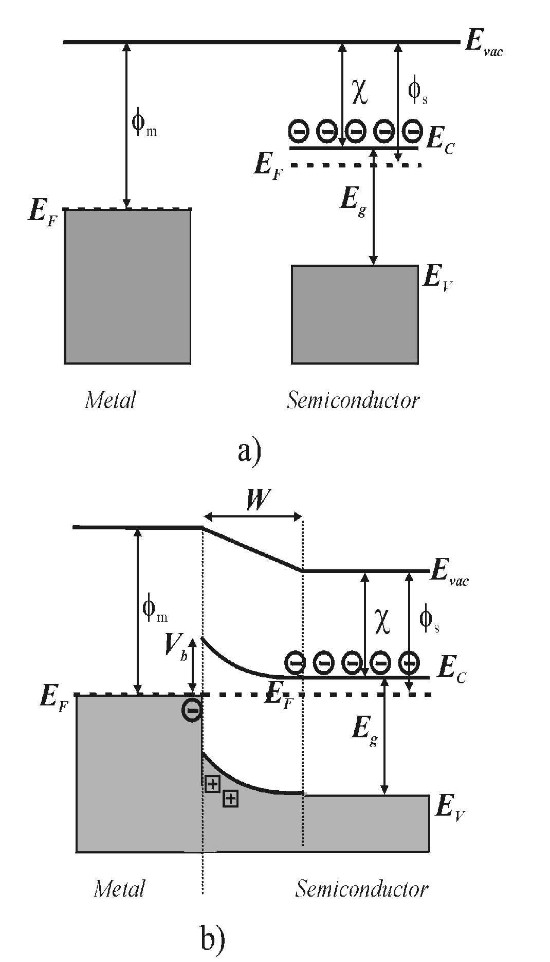
\includegraphics[width=0.8\textwidth,height=10\baselineskip,keepaspectratio]{ch3/image3} 
	\caption{Bruit dans un amplificateur opérationnel} 
	\label{fig:bruitaop}
\end{figure}
\paragraph{Remarques:} Les courants \(i_{b^\pm} \neq\) courant de bias (= courant constant de polarisation). \(i_{b^\pm}\) sont des courants à moyenne nulle, allant vers le circuit et dont l'impact dépend de l'impédance (+ l'impédance est grande, + le bruit est grand).
\subsection{Limitation de bruit}
\subsubsection{Introduction et principales techniques}
Le but de cette sous-section est de développer des méthodes afin de rendre l'amplitude du bruit négligeable face à celle du signal, c-à-d \(\nearrow\) SNR. Pour ce faire, il est possible d'agir sur 2 choses:
\begin{enumerate}
	\item Augmenter le signal, c-à-d amplifier dès que possible et autant que possible le signal \(\Rightarrow\) pré-ampli à grand gain et faible bruit.
	\item Réduire le bruit de tous les composants.
\end{enumerate}
Afin de parvenir à un résultat, il est important de suivre ces quelques règles de base:
\begin{enumerate}
	\item Cibler le type de bruit (afin de choisir des contre-mesures efficaces).
	\item S'attaquer au bruit prépondérant (on va peut-être s'occuper du gros d'abord, non ?).
	\item S'attaquer au bruit dès que possible (chaque module apportant son propre bruit (irréversible), il devient impossible de séparer les bruits entre eux au fur et à mesure que l'on avance sur la chaîne)
\end{enumerate}
Nous pouvons agir:
\begin{description}
\item \emph{Au niveau des composants:}
\begin{itemize}
	\item Choisir des composants à faible bruit.
	\item Jouer sur les paramètres influençant directement le bruit (ex. réduire la température pour un bruit thermique).
\end{itemize}
\item \emph{Au niveau du système:}
\begin{itemize}
	\item \hyperref[subsubsec:entreenobruit]{Pré-ampli à faible bruit} (parfois étage à transistor discrets afin de minimiser le bruit de l'aop, lui-même constitué d'un nombre conséquent de transistors discrets).
	\item \nameref{subsubsec:bandepass} (réduire le bruit dans un bande passante plus restreinte).
	\item \nameref{subsubsec:résistsource}.
	\item \nameref{subsubsec:detectsync} pour le bruit rose.
\end{itemize}
\end{description}
\subsubsection{Réduire la bande passante} \label{subsubsec:bandepass}
Le bruit à virtuellement une bande passante infinie alors que celle du dispositif de mesure est limitée \(\Rightarrow\) bruit perçu limité à la bande passante du dispositif.\bigbreak

Pour un bruit blanc de densité \(e_{bb}\) perçu au travers d'une bande passante \(B=f_{\text{max}}-f_{\text{min}}\):
\begin{equation}
E_b^2 = \int_{f_{\text{min}}}^{f_{\text{max}}} dE_b^2 = \int_{f_{\text{min}}}^{f_{\text{max}}} e_{bb}^2\,df = e_{bb}^2(f_{\text{max}}-f_{\text{min}}) 
\end{equation}
Ainsi, la valeur efficace du bruit dans une bande de fréquence, permettant d'avoir une idée sur l'amplitude du bruit, est:
\begin{equation}\label{eq:valeffbruitDB}
E_b = e_{bb}\sqrt{B}
\end{equation}
On déduit de \eqref{eq:valeffbruitDB} que plus la bande passante du dispositif de mesure \(\nearrow\), plus le bruit présent à la sortie de la chaîne de mesure \(\nearrow\) et donc plus le signal est perturbé. \(\Rightarrow\) Il faut \textbf{limiter la bande passante} (filtrage).\bigbreak

Dans un dispositif réel, le bruit est un "bruit composite" (rose (aux basses fréquences) + blanc (aux hautes fréquences)). Le point où les 2 densités spectrales sont égales (rose \(\cup\) blanc) est appelé la \emph{fréquence coin}.
\begin{figure}[H]
	\centering
	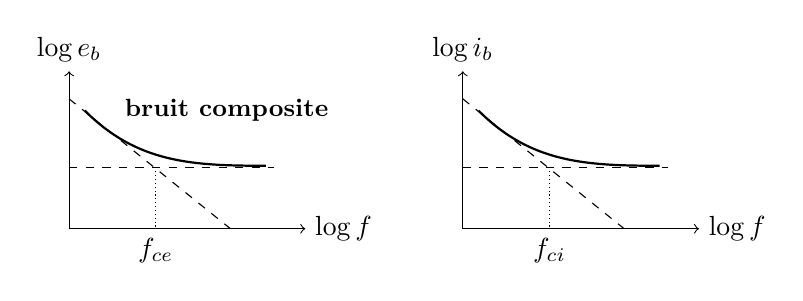
\begin{tikzpicture}
		\draw[dashed] (0,1.65) -- (2.05,0);
		\draw[dashed] (0,0.78) -- (2.6,0.78);
		\draw[densely dotted] (1.1,0.78) -- (1.1,0) node[below]{\(f_{ce}\)};
		\draw[thick] (0.2,1.5) to[out=-45, in=180] (2.5,0.8);
		\draw[->] (0,0) -- (0,2) node[above]{\(\log e_b\)};
		\draw[->] (0,0) -- (3,0) node[right]{\(\log f\)};
		\draw (2,1.5) node{\textbf{\small bruit composite}};
		\draw[dashed] (5,1.65) -- (7.05,0);
		\draw[dashed] (5,0.78) -- (7.6,0.78);
		\draw[densely dotted] (6.1,0.78) -- (6.1,0) node[below]{\(f_{ci}\)};
		\draw[thick] (5.2,1.5) to[out=-45, in=180] (7.5,0.8);
		\draw[->] (5,0) -- (5,2) node[above]{\(\log i_b\)};
		\draw[->] (5,0) -- (8,0) node[right]{\(\log f\)};
		\end{tikzpicture}
\end{figure}
La valeur efficace de bruit composite dans la bande passante est :
\begin{equation}
E_b^2 = e_{bb}^2\left[(f_{\text{max}}-f_{\text{min}})+f_{ce}\ln\left(\frac{f_{\text{max}}}{f_{\text{min}}}\right)\right]
\end{equation}
Ainsi, pour réduire le bruit il faut:
\begin{itemize}
	\item limiter la bande passante (\(f_{\text{max}}-f_{\text{min}}\))
	\item choisir des composants pour minimiser:
	\begin{itemize}
		\item la densité spectrale de bruit blanc \(e_{bb}\text{ (et }i_{bb}\))
		\item la fréquence de coupure \(f_{ce}\text{ (et }f_{ci}\))
	\end{itemize}
\end{itemize}
\subsubsection{Résistance de source} \label{subsubsec:résistsource}
\begin{description}
	\item[\(R_s\)] résistance de sortie du capteur (ou de l'étage précédent)
\end{description}
Un AOP comprend des sources de tension de bruit et de courant de bruit, il faut donc choisir un ampli à:
\begin{itemize}
	\item faible tension de bruit lorsque \(R_s\) est faible
	\item faible courant de bruit lorsque \(R_s\) est élevée
\end{itemize}
\subsubsection{Étage d'entrée à faible bruit} \label{subsubsec:entreenobruit}
Comparons 2 cas possible d'étage d'entrée de gain total \(G\):\bigbreak
\underline{Amplificateur unique:}  soit sa densité spectrale de bruit ramené à l'entrée \(v_b^{in}\), le bruit total à la sortie vaut
\begin{equation}\label{eq:etasortieunique}
v_b^{out}=G . v_b^{in}
\end{equation}
\underline{Ajout d'un étage d'entrée à faible bruit:} soit un 1\up{er} étage d'entrée de gain \(G_1\) et de densité spectrale de bruit (entrée) \(v_{b_1}^{in}\) et un 2\up{ème} étage de gain \(G_2\) et de densité spectrale de bruit (entrée) \(v_{b_2}^{in}\) tel que \(G_1 . G_2 = G\). Nous aurons donc à la sortie du premier étage:
\begin{itemize}
	\item le bruit dû au 1\up{er} étage: \(v_{b_1}^{out}=G_1 . v_{b_1}^{in}\)
	\item le bruit dû au 2\up{ème} étage: \(v_{b_2}^{in}\)
\end{itemize}
Et donc, le bruit total à la sortie vaut:
\begin{equation}\label{eq:etasortie}
v_b^{out} = G_2\sqrt{\left(v_{b_1}^{out}\right)^2 + \left(v_{b_2}^{in}\right)^2} = G\sqrt{\left(v_{b_1}^{in}\right)^2 + \left(v_{b_2}^{in}/G_1\right)^2}
\end{equation}
On remarque que le bruit total de \eqref{eq:etasortie} sera plus faible que celui de \eqref{eq:etasortieunique} si \(G_1\gg 1\text{ et } v_{b_1}^{in}<v_b^{in}\)
\begin{center}
	\textbf{le bruit d'un ampli est minimisé en plaçant en tête un préamplificateur à faible bruit et de gain suffisant}
\end{center}
\subsubsection{Détection synchrone} \label{subsubsec:detectsync}
Si le signal utile se situe à basse fréquence, le bruit en 1/f (rose) domine \(\Rightarrow\) transposer momentanément le signal utile à une fréquence plus élevée, à l'aide d'une modulation d'amplitude (signal sera au alentour de la fréquence porteuse), afin de réaliser la transmission ou l'amplification en dehors de la bande bruitée. 
\begin{figure}[H] 
	\centering 
	\begin{tikzpicture}
	 	\draw plot[domain=0:3*pi] (\x,{0.6*sin(\x r)}) node[right]{signal};
	 	\draw plot[samples=300,domain=0:3*pi] (\x,{0.6*sin(20*\x r)*(1+0.6*sin(\x r)) -2}) node[right]{AM};
	 	\node[draw,ellipse] (C) at (-0.5,-4){capteur};
	 	\node[draw] (M) at (2.5,-4){modulation};
	 	\node[draw] (A) at (5,-4){ampli};
	 	\node[draw] (D) at (7.5,-4){démodulation};
	 	\node[draw] (P) at (10.5,-4){Passe-bas};
	 	\draw[->, >=latex'] (C) -- (M);
	 	\draw[->, >=latex'] (M) -- (A);
	 	\draw[->, >=latex'] (A) -- (D);
	 	\draw[->, >=latex'] (D) -- (P);
	\end{tikzpicture} 
	\caption{Détection synchrone} 
\end{figure}
Pour résumer:
\begin{itemize}
		\item {\makebox[4cm]{signal utile:\hfill} \(s(t)\)}
		\item {\makebox[4cm]{signal modulation:\hfill} \(u_{mod}(t)=\cos(2\pi f_ut)\)}
		\item {\makebox[4cm]{signal démodulation:\hfill} \(u_{demod}(t) = \cos(2\pi f_ut+\varphi)\)}
\end{itemize}\ \\
Et donc, le signal modulé vaut:
\begin{equation}
s_{mod}(t) = s(t) . u_{mod}(t)
\end{equation}
qui est bien transposé autour de la fréquence \(f_u\) (\(f_u\gg f_{max}\)). Pour démoduler, nous utilisons une démodulation synchrone, c-à-d en multipliant par la même sinusoïde que lors de la modulation (+ déphasage inévitable \(\varphi\))
\begin{equation}
\begin{split}
s_{demod}(t) &= s_{mod}(t) . u_{demod}(t)\\
&= s(t)\cos(2\pi f_u t)\cos(2\pi f_u t+\varphi)\\
&= s(t)\frac{1}{2}\{\underbrace{\cos\varphi}_{\cst}+\cos(4\pi f_u t+\varphi)\}
\end{split}
\end{equation}
qui, après un filtre passe-bas (\(f_c \approx f_{max}\)) devient:
\begin{equation}
s_{demod}'(t) = s(t)\frac{\cos\varphi}{2}
\end{equation}
\section{Les parasites}
\subsection{Introduction}
Les parasites sont des tensions ou courants indésirables, d'origine extérieure à l'appareil perturbé, se superposant au signal utile. Ceux-ci apparaissent par suite du couplage d'un circuit source avec le circuit perturbé (victime).\bigbreak

L'origine physique le plus courant de ces parasites sont les parasites électromagnétiques (expliqués par les équations de Maxwell). Toutes charges et courants génèrent des champs (\(E\) et \(H\) variables, formant une onde électromagnétique) qui se transforment en f.e.m. (\(\int E\) ou \(H\) loi de Lenz). Il existe néanmoins d'autres phénomènes physiques comme la thermoélectricité, la piézoélectricité, etc.\bigbreak

À cela se rajoute le concept de champ proche et champ lointain ainsi que le type de couplages (C.f \autoref{fig:champproloin} et \autoref{fig:typcouplage})
\begin{figure}[H] 
	\centering 
	\includegraphics[width=0.8\textwidth,height=10\baselineskip,keepaspectratio]{ch3/image4} 
	\caption{Champ proche et champ lointain} 
	\label{fig:champproloin}
\end{figure}
\begin{figure}[H] 
	\centering 
	\includegraphics[width=0.8\textwidth,height=10\baselineskip,keepaspectratio]{ch3/image5} 
	\caption{Type de couplages}
	\label{fig:typcouplage} 
\end{figure}
Quelques exemples de parasites sont cités slide 46.
\subsection{Parasites rayonnés}
\subsubsection{Couplage capacitif}
Les charges portées par un conducteur induisent des charges opposées (\(\Rightarrow\) courant) dans un autre conducteur via le champ électrostatique \(E\). Existe entre toute paire de conducteurs et est modélisé par une capacité parasite entre ces conducteurs. À prendre en compte dans le domaine du \textbf{champ proche} (\(L<\lambda/2\pi\)). Ex.: pistes proches ou superposée dans les circuits imprimés, les bus, etc.\bigbreak

\(\Rightarrow\) éviter les lignes parallèles, éloigner le plus possible les fils les uns des autres afin de réduire les capacités parasites ou disposer d'un blindage électrostatique (décrit plus bas).

Un cas particulier existe, les \textbf{décharges électrostatiques}:
\begin{description}
	\item[définition] claquage de l'isolant entre les armatures du condensateur parasite lorsque le champs électrique devient trop important
	\item[exemple] tapis, vêtement en laine, éclair en cas d'orage, claquage de l'oxyde de grille dans les circuits MOS
	\item[contre-mesure] mise à la terre des dispositifs/utilisateurs pour les décharger et éviter l'accumulation de charge, intégrer un dispositifs de dissipation de puissance (parasurtenseurs, décrit plus bas)
\end{description}
Un exemple de dispositif permettant d'empêcher l'accumulation de charge se trouve \autoref{fig:dispdechdio}. La diode protectrice protège le circuit en aval en permettant le passage du courant parasite en cas de surtension.
\begin{figure}[H] 
	\centering
	\begin{circuitikz}
	\draw (0,0) node[left]{\SI{0}{\volt}} to[short] (4,0) to[open] (4,1) to[short] (0,1) node[left]{\SI{5}{\volt}};
	\draw (2,0) to[sDo,l_=\SI{6}{\volt}] (2,1);
	\end{circuitikz}
	\caption{Dispositif de décharge} 
	\label{fig:dispdechdio}
\end{figure}
\subsubsection{Couplage inductif}
Un champ magnétique variable induit dans un conducteur une f.e.m. qui tend à s'opposer à cette variation (loi de Lenz). Existe en théorie dans toute paire de conducteur et est modélisé par une inductance mutuelle parasite entre ces conducteurs. À prendre en compte dans le domaine du \textbf{champ proche} (\(L<\lambda/2\pi\)). Ex.: lignes de signal (téléphone, instrumentation) entre elles ou placées à coté d'une ligne d'alimentation/moteur électrique etc.\bigbreak

Il faut donc éloigner les sources de champ magnétique, minimiser la surface offerte au champ magnétique extérieure (réduire l'inductance mutuelle en jouant sur l'orientation spatiale ou sur la surface de la boucle, en tressant les câbles par exemple), implémenter un blindage magnétique (décris plus bas).\\
Mode de couplage le plus répandu, toute boucle formée de conducteur est une victime potentielle. Phénomène d'autant plus critique que la fréquence est élevée. 

Un cas particulier, les \textbf{câbles de transmission}. Ceux-ci forment une boucle et sont donc des victimes privilégiés. Il existe quelques contre-mesures:
\begin{itemize}
	\item réduire la surface de la boucle:
	\begin{itemize}
		\item réduire la longueur des câbles
		\item rapprocher les conducteurs aller et retour
		\item torsader les fils d'amenée et de retour. Si au-delà des quelques \si{\mega\hertz}, passer au câble coaxial (mutuelle nulle).
	\end{itemize}
	\item câbles blindés
	\item passer à une transmission ayant une meilleur immunité:
	\begin{itemize}
		\item boucle de courant (si la transmission est en courant, il n'y a pas d'impact)
		\item porter l'information sur la fréquence
		\item passer au numérique
		\item code détecteurs/correcteurs d'erreur
	\end{itemize}
\end{itemize}

\subsubsection{Couplage électromagnétique}
Dans le domaine du \textbf{champ lointain} (\(L>\lambda/2\pi\)), \(E\) et \(H\) coexistent sous forme d'une onde plane. Tout conducteur peut se comporter comme une antenne réceptrice parasite à l'onde plane. C'est d'autant plus critique que la fréquence est élevée. Ex.: GSM dans les hôpitaux ou les avions etc.\bigbreak

Il faut donc limiter la source d'émission, implémenter un blindage EM (plus bas), designer le circuit récepteur, ou  utiliser un dispositif optique (comme la fibre optique).
\subsubsection{Blindage}
\underline{\textit{Blindage électrostatique} (champ proche)}: utiliser un matériau conducteur dont le potentiel est imposé. Ceci offre un chemin de retour pour le courant parasite et évite de modifier le potentiel du circuit victime. Le plus souvent, c'est une mise à la terre via une impédance faible. Ex.: blindage complet (boîtier) ou \autoref{fig:blindelectrostat}.\\
Il faut bien comprendre ici qu'au lieu de réduire la capacité parasite, nous interposons des conducteurs supplémentaires dont le potentiel est fixé. De plus, rien ne nous interdit de fixer un potentiel différent de la masse/terre (\SI{0}{\volt})
\begin{figure}[H] 
	\centering 
	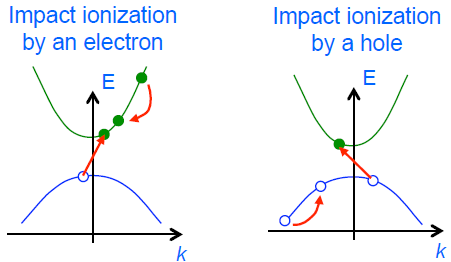
\includegraphics[width=0.7\textwidth,height=10\baselineskip,keepaspectratio]{ch3/image6} 
	\caption{Forme de blindage électrostatique}
	\label{fig:blindelectrostat}
\end{figure}
\begin{figure}[H] 
	\centering 
	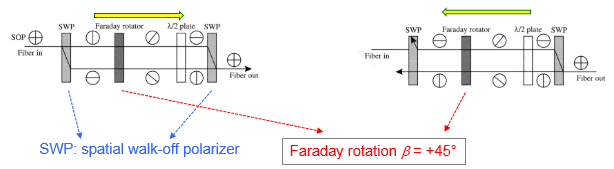
\includegraphics[width=0.8\textwidth,height=10\baselineskip,keepaspectratio]{ch3/image7} 
	\caption{Blindage électrostatique}
\end{figure}
\underline{\textit{Blindage magnétique} (champ proche)}: ici nous avons 2 cas:
\begin{itemize}
	\item champ BF: matériau ferromagnétique (\(\mu\) élevé). Il dévie les lignes de champ magnétique, mais il faut faire attention à la saturation \(\Rightarrow\) grande épaisseur du ferromagnétique (mais cher et lourd) (\autoref{fig:blindmagn}).
	\item champ HF: matériau conducteur (non ferromagnétique). les courants de Foucault induits dans le blindage s'opposent à la pénétration du champ extérieur.
\end{itemize}
\begin{figure}[H] 
	\centering 
	\includegraphics[height=4\baselineskip]{ch3/image8} 
	\caption{Blindage ferromagnétique}
	\label{fig:blindmagn}
\end{figure}

\underline{\textit{Blindage EM} (champ lointain)}: utiliser un matériau conducteur qui supprimera le champ perturbateur par un champ opposé induit (courant de Foucault). Typiquement, une cage de Faraday. Néanmoins, il nécessite de faire rentrer les lignes de signal et d'alimentation (coucou couplage inductif) et la moindre ouverture réduit l'efficacité du blindage \(\Rightarrow\) construction très délicate.\bigbreak

\underline{\textit{Remarques générales}}: Les blindages concerne tout autant les câbles de transmission que les boîtiers (capteur, instrumentation). De plus la connections des blindages de câbles n'est pas trivial.
\subsection{Parasites conduits}
\subsubsection{Introduction}
Commençons pas définir ce qu'est un \emph{couplage galvanique}:
\begin{description}
	\item[définition] transmission d'un signal perturbateur entre la source de ce signal et le dispositif victime \emph{via un conducteur commun}.
\end{description}
Ceci concerne autant les lignes de signal que les alims/masse/terre et le simple fait de brancher 2 appareils sur le réseau électrique établit un couplage galvanique. Comme par exemple 2 appareils à \SI{220}{\volt} dans 2 pièces différentes, connectés à la masse. Si l'un demande en puissance, cela fait baisser la tension dans tout le circuit. Il existe 2 origines distinctes:
\begin{enumerate}
	\item le conducteur commun (idéal) transmet un signal parasite issu d'un autre équipement (comme parasite transmis via les lignes d'alimentation à cause de la foudre).
	\item le conducteur commun n'est pas équipotentiel \(\Rightarrow\) la circulation d'un courant sur ce conducteur génère des f.e.m. parasites.
\end{enumerate}
Ces 2 origines sont bien évidement cumulables. Il existe 2 niveaux de conséquences:
\begin{enumerate}
	\item dégrade le signal (superposition du signal utile et parasite, si sur alim \(\rightarrow\) mauvais fonctionnement du circuit).
	\item détruit l'équipement (surtension (claquage électrostatique) ou surpuissance (destruction par échauffement)).
\end{enumerate}
Remarquons que tout parasite rayonné devient f.e.m. ou courant sur un conducteur et donc que les conséquences sont aussi valables pour les parasites rayonnés en amont.
\subsubsection{Contre-mesures}
Il existe 3 contre-mesures générales:
\begin{enumerate}
	\item Contre les parasites conduits issus d'autres équipement:
	\begin{itemize}
		\item filtre passe-bas pour le spectre étendu, filtre réjecteur de fréquence pour le spectre étroit
		\item équilibrer (rendre le circuit plus symétrique, voir plus bas)
	\end{itemize}
 \hspace*{\dimexpr\linewidth-\textwidth\relax}%
 \begin{minipage}[t]{\textwidth}%
 	Néanmoins, il n'est pas trivial de réaliser le filtre, nous pouvons utiliser un filtre passif (capa et inductance) ou actif (passif + AOP), en mode commun ou différentiel.
 \end{minipage} 
	\item Contre les parasites générés par l'impédance des connexions:
	\begin{itemize}
		\item design des connexions (\(\searrow\) longueur + \(\nearrow\) section conductrice \(= \searrow\) impédance)
		\item connecter judicieusement les alimentations et les masses:
		\begin{enumerate}
			\item éviter les chemins communs \(\Rightarrow\) câblages en étoile
			\item séparer alimentations de signaux à fréquence et/ou puissance \(\neq\)
		\end{enumerate}	
	\end{itemize}
	\item Contre la destruction des équipement par surtension/surpuissance \(\Rightarrow\) parasurtenseurs, dont le principe est de limiter la tension  et ayant la capacité de dissiper l'énergie excédentaire:
	\begin{itemize}
		\item diodes Zener utilisée en avalanche (protection)
		\item varistance (résistance non linéaire, \(\nearrow\) tension \(= \searrow\) résistance)
		\item éclateurs (tube à gaz dissipant temporairement l'énergie via un arc électrique)
	\end{itemize}
\end{enumerate}
\underline{\textit{Exemple} (flemme)}:
\begin{figure}[H] 
	\centering 
	\includegraphics[width=0.8\textwidth,height=10\baselineskip,keepaspectratio]{ch3/image9} 
	\caption{Circuit électronique initial} 
\end{figure}
A première vue, les fils ou pistes d'alimentation sont des équipotentielles. En réalité, il existe souvent une distance de plusieurs centimètres ou dizaines de centimètres entre les bornes d'alimentation d'une carte électronique et le circuit intégré le plus éloigné.\\
L'impédance de ces connections joue un rôle non négligeable:
\begin{itemize}
\item la chute de tension ohmique due à la résistance des connections (l'épaisseur des piste est très faible: de l'ordre de \SI{30}{\micro\meter}) parcourue par le courant moyen.
\item les fluctuations de tension liées aux variations de courant importantes (basculement de portes, charge de capacités parasites, "réveil" d'un circuit CMOS) sur l'inductance des connections \(\rightarrow\) peuvent faire sortir l'alimentation de sa plage normale.
\end{itemize}
\begin{figure}[H] 
	\centering 
	\includegraphics[width=0.8\textwidth,height=10\baselineskip,keepaspectratio]{ch3/image10} 
	\caption{Circuit électronique final} 
\end{figure}
Les améliorations les plus courantes de l'alimentation sont
\begin{itemize}
\item l'utilisation de fils de plus forte section ou de pistes plus larges (quelques \si{\milli\meter}) ou de circuits multi-couches (permettant d'inclure plan de masse et plan d'alimentation)
\item les condensateurs de découplage sous forme
\begin{itemize}
	\item d'un condensateur électrolytique (généralement quelques \si{\micro\farad}) 
	\item d'un ensemble de condensateurs de très bonne qualité disséminés sur toute la carte, le plus près possible des pattes d'alimentation de chaque gros circuit intégré et de chaque groupe de petits circuits

\end{itemize}
\item une diode Zener (protection contre les surtensions)
\end{itemize}
Les condensateurs constituent des sources de tension localisée (à très court terme) vis-à-vis des impulsions de courant consommées par les circuits intégrés.\bigbreak

Le mot "découplage" qualifie le fait que les variations de consommation (composante alternative) propres du circuit ne sont pas vues par les fils d'alimentation, qui ne véhiculent que la composante continue (moyenne). Les inductances parasites du câblage ont donc beaucoup moins d'influence.\bigbreak

La diode Zener permet d'écrêter les surtensions transitoires. Si celles-ci sont répétitives, l'absorption d'énergie par la Zener peut excéder ses capacités de refroidissement et la détruire. En cas de tension d'entrée trop importante, la Zener va également surchauffer et fondre, généralement en court-circuit, ce qui protégera les circuits coûteux en aval.
\subsubsection{Isolation galvanique}
\begin{description}
	\item[définition] coupure de tout lien galvanique entre 2 parties du montage
	\item[moyen] couplage magnétique (transformateur) et couplage optique (optocoupleur, fibre optique)
\end{description}
C'est souvent nécessaire pour des raisons de protection des utilisateurs et des équipements (sécurité). Le but est de faire passer de la puissance/info d'une autre manière que via de l'électricité.
\iffalse \subsection{Compatibilité électromagnétique}
\begin{description}
	\item[définition] discipline ayant pour but d'analyser et de résoudre l'ensemble des problèmes de parasitage EM d'un équipement par un autre
\end{description}
C'est une discipline de plus en plus importante en raison de la multiplications des équipement électroniques. Il existe des normes stricte depuis les années 90. On définit:
\begin{description}
	\item[CEM/EMC] compatibilité EM
	\item[IEM/EMI] interférence EM
\end{description}
\subsection{Notions embrassées par la CEM}
les normes CEM, les types de couplages, les imperfections des composants (passif et surtout actifs car sources de perturbations), les boîtiers et blindages, le câblage, le routage des pistes dans les circuits imprimés (surtout masse et alim) et « tous les effets du second ordre ».
\subsection{Exemple: alimentation à découpage}
Exemple slide 81--85.\fi
\section{Câblage et connexions}
\subsection{Référence d'un signal}
Rappel sur tension et masse slide 88. Nous ajoutons quelques subtilités:
\begin{enumerate}
	\item impédance de masse: en pratique la "masse" d'un montage peut être un conducteur ayant une certaine extension physique \(\Rightarrow\) impédance \(\neq 0 \Rightarrow\) lorsque parcouru par un courant, pas équipotentiel \(\Rightarrow\) plus vraiment une masse (f.e.m. parasite)
	\item plusieurs montages: les masses de différents montages sont à priori pas au même potentiel (pas connecté ou connecté via des impédance \(\neq 0\))
\end{enumerate}
Pour rappel, la mise à terre est une connexion d'un conducteur au potentiel de la terre (sol) afin d'assurer la protection des utilisateurs et des équipements (le réseau de terre doit avoir l'impédance la plus faible possible). La masse (référence) et la terre (protection) ne sont pas forcément connectées.\bigbreak

On définit les appareils:
\begin{description}
	\item[flottants] aucune des 2 bornes du signal (entrée ou sortie) n'est connectée à la terre (appareils portatifs, appareils sur réseau à 3 bornes)
	\item[non flottants] masse = terre
\end{description}
\subsection{Montage "single-ended"}
\subsubsection{Cas idéal}
Un montage "single-ended" possèdent les caractéristiques suivantes:
\begin{itemize}
\item un amplificateur "single-ended" (= asymétrique) comme un (non-)inverseur, suiveur à AOP. Au niveau multiplexage, il faut \(N+1\) fils pour \(N\) signaux. \item La référence du capteur = la référence de l'instrumentation
\end{itemize} 
Dans le cas théorique \(V_{in}=e_s\) (donc pas de parasites).
\begin{figure}[H] 
	\centering 
	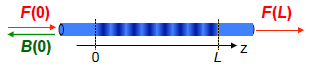
\includegraphics[width=0.8\textwidth,height=10\baselineskip,keepaspectratio]{ch3/image11} 
	\caption{Single-ended (idéal)} 
\end{figure}
\subsubsection{Cas réel}
Dans le cas réel, une source parasite \(e_p\) vient s'ajouter car il existe une impédance de masse non négligeable et des parasites induits dans la boucle. Il en résulte \(V_{in} = e_s + e_p\) et donc un signal dégradé.
\begin{figure}[H]
	\centering 
	\includegraphics[width=0.8\textwidth,height=10\baselineskip,keepaspectratio]{ch3/image12} 
	\caption{Single-ended (réel)} 
\end{figure}
\(\Rightarrow\) éviter les montages "single-ended". Sauf si la chute de tension sur l'impédance de masse ET les f.e.m induites sont négligeables, comme pour:
\begin{itemize}
	\item un capteur proche de l'ampli
	\item un capteur éloigné mais isolé de son environnement et sa masse est ramenée à l'ampli par une connexion d'impédance négligeable
\end{itemize}
\subsection{Montage différentiel}
\begin{figure}[H] 
	\centering 
	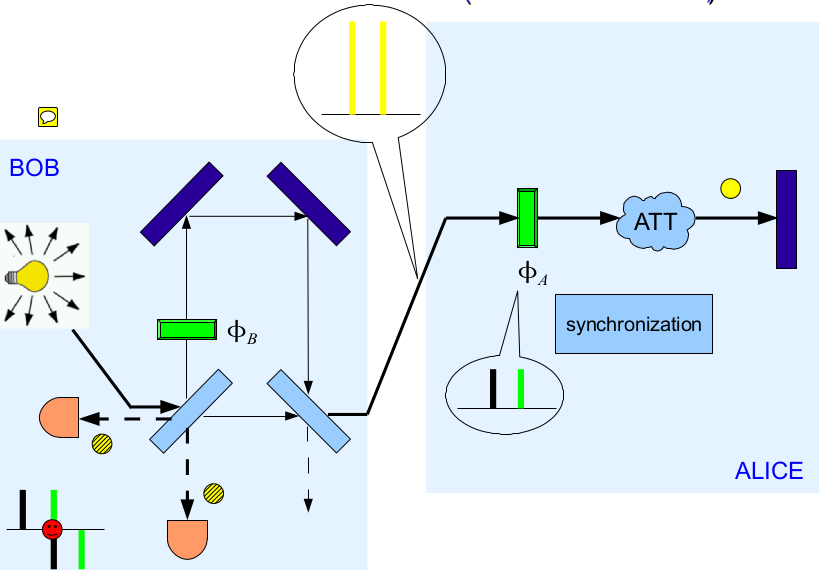
\includegraphics[width=0.8\textwidth,height=10\baselineskip,keepaspectratio]{ch3/image13} 
	\caption{Montage différentiel} 
\end{figure}
Dans ce montage, nous avons:
\begin{itemize}
		\item {\makebox[8cm]{tension d'entrée de l'ampli différentiel\hfill} \(V^-=e_p\qquad V^+=e_s+e_p\)} 
		\item {\makebox[8cm]{tension différentielle\hfill} \(V_{md} = V^+-V^-=e_s\)} 
		\item {\makebox[8cm]{tension de mode commun (parasites)\hfill} \(V_{mc}=\frac{V^++V^-}{2}=e_p+\frac{e_s}{2}\)} 
		\item {\makebox[8cm]{tension de sortie\hfill} \(V_{out}=A_{md}V_{md}+A_{mc}V_{mc}\)} 
		\item {\makebox[8cm]{taux de réjection en mode commum\hfill} \(\text{CMRR} = \frac{A_{md}}{A_{mc}}\)} 
\end{itemize}
Il faut donc maximiser le CMRR (common mode rejection ratio). On en déduit les avantages et inconvénients suivants:
\begin{description}
	\item[avantages]:
	\begin{itemize}
		\item les parasites de mode commun, les parasites par couplage galvanique et les autres parasites induits en mode commun sont rejetés
		\item signal dont aucune des bornes ne peut être considérée comme une masse (même imparfaite). ex: tension de déséquilibre d'un pont de Wheatstone ou un montage porté à une tension élevée.
	\end{itemize}
	\item [inconvénients]:
	\begin{itemize}
		\item les parasites de mode différentiel sont toujours amplifiés
		\item liaison \(2N\) (ou \(2N+1\)) fils pour \(N\) signaux
	\end{itemize}
\end{description}
\underline{\textit{Remarques}}: en instrumentation, la tension de mode commun est souvent du même ordre de grandeur  voir plus élevée que la tension différentielle. On essayera de faire apparaître les parasites sous forme de tension en mode commun car elles seront rejetés (pas entièrement, dépend du CMRR). Hélas, un bon CMRR ne suffit pas.
\begin{figure}[H] 
	\centering 
	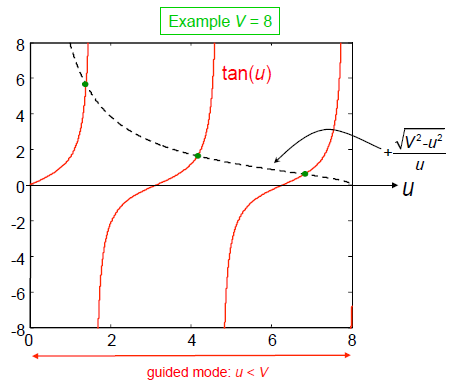
\includegraphics[width=0.8\textwidth,height=10\baselineskip,keepaspectratio]{ch3/image14} 
\end{figure}
Pour un multiplexeur, les deux montages s'implémentent comme illustré à la \autoref{fig:multmont}
\begin{figure}[H]
	\centering
	\subfigure[Single-ended]{\label{fig:multsing}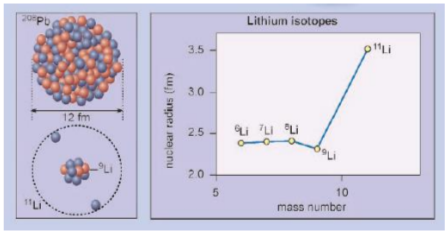
\includegraphics[width=0.4\textwidth]{ch3/image15}}
	\subfigure[Différentiel]{\label{fig:mutldiff}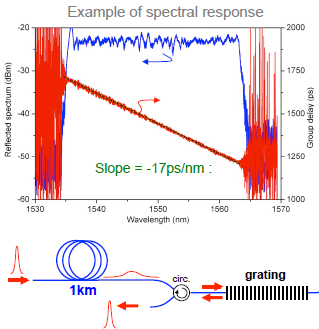
\includegraphics[height=15\baselineskip]{ch3/image16}}
	\caption{Implémentation avec un multiplexeur}
	\label{fig:multmont}
\end{figure}
\subsection{Symétrie des voies d'amenée}
\subsubsection{Déséquilibre série}
\begin{figure}[H] 
	\centering 
	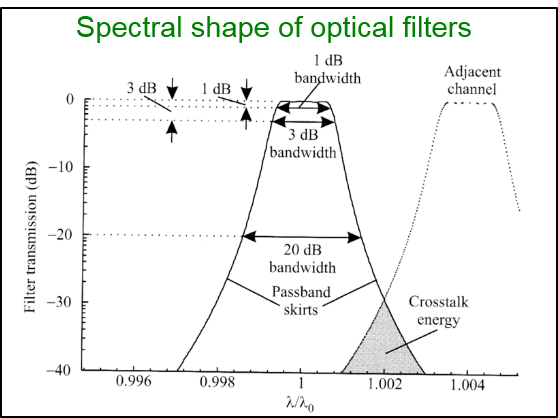
\includegraphics[width=0.8\textwidth,height=10\baselineskip,keepaspectratio]{ch3/image17} 
	\caption{Déséquilibre série} 
\end{figure}
Soit \(Z_1, Z_2\) les impédances série des voies d'amenée (souvent résistif) et soit un ampli différentiel ayant comme impédances d'entrée:
\begin{itemize}
	\item 1 impédance différentielle \(Z_d\) (hyp: \(\infty\))
	\item 2 impédances mode commun \(Z_{mc}\) (hyp: identiques)
\end{itemize}
Souvent \(Z_{mc} = \SI{e10}{\ohm}\)  \(\parallelsum\) capa en \si{\pico\farad} \(\Rightarrow \text{ passe-bas }f_c\approx \SI{10}{\hertz}\). Nous avons donc:
\[v_d = v_2-v_1\qquad v_d'=v^+-v^-\qquad v_{mc}=\frac{v_1+v_2}{2}\qquad v_{mc}'=\frac{v^++v^-}{2}\]
Les tensions à l'entrée de l'ampli sont:
\[v^-=\frac{Z_{mc}}{Z_1+Z_{mc}}v_1\qquad v^+=\frac{Z_{mc}}{Z_2+Z_{mc}}v_2\]
en faisant l'hypothèse que \(Z_{mc}\gg Z_1, Z_2\):
\[v_{mc}'\approx v_{mc}\qquad v_d'=v_d+\frac{Z_1-Z_2}{Z_{mc}}v_{mc}\]
La tension différentielle est polluée par une fraction de la tension de mode commun, fraction d'autant plus importante que \(Z_1\text{ et }Z_2\) sont \(\neq\) et que \(Z_{mc}\) est petit. Tout déséquilibre engendrera une dégradation du CMRR. En particulier, il faut que \(R_1=R_2\) pour une bonne réjection des tensions de mode commun continues et basse fréquence.
\subsubsection{Déséquilibre parallèle}
\begin{figure}[H] 
	\centering 
	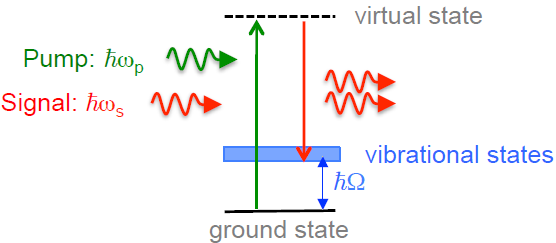
\includegraphics[width=0.8\textwidth,height=10\baselineskip,keepaspectratio]{ch3/image18} 
	\caption{Désiquilibre parallèle} 
\end{figure}
On ajoute maintenant \(C_1', C_2'\) des capa parasites \(\parallelsum\) venant s'ajouter aux 2 capas \(C_{mc}\) de l'ampli. Nous avons donc:
\[C_1=C_1'+C_{mc}\qquad C_2=C_2'+C_{mc}\] 
\begin{figure}[H] 
	\centering 
	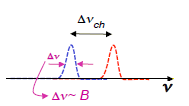
\includegraphics[width=0.8\textwidth,height=10\baselineskip,keepaspectratio]{ch3/image19}
\end{figure}
En supposant toujours que \(Z_d\gg\)
\[v^-=\frac{(R_{mc} \parallelsum C_1)}{R_1+(R_{mc} \parallelsum C_1)}\qquad v^+=\frac{(R_{mc} \parallelsum C_2)}{R_2+(R_{mc} \parallelsum C_2)}\] 
Dans la gamme de fréquence \(\frac{1}{R_{mc}C_1},\frac{1}{R_{mc}C_2}\ll\omega_{mc}\ll\frac{1}{R_1C_1},\frac{1}{R_2C_2}\) on a:
\[v_{mc}'\approx v_{mc}\qquad v_d'=v_d+j\omega(R_1C_1-R_2C_2)v_{mc}\]
La tension différentielle est polluée par une fraction de la tension de mode commun, fraction d'autant plus importante que \(C_1\text{ et }C_2\) sont différentes, mais cette fois, c'est surtout pour les fréquences plus élevées.\bigbreak

En pratique, \(C_1'\text{ et }C_2'\) sont des capas parasites qui existent vis-à-vis du blindage électrostatique des voies d'amenée, alors que précédemment, on a fait l'hypothèse d'être à la masse. En portant le blindage à la tension de mode commun \(v_{mc}\), on annule la tension différentielle parasite due au déséquilibre de \(C_1', C_2'\), c'est la \emph{garde}.
\begin{figure}[H] 
	\centering 
	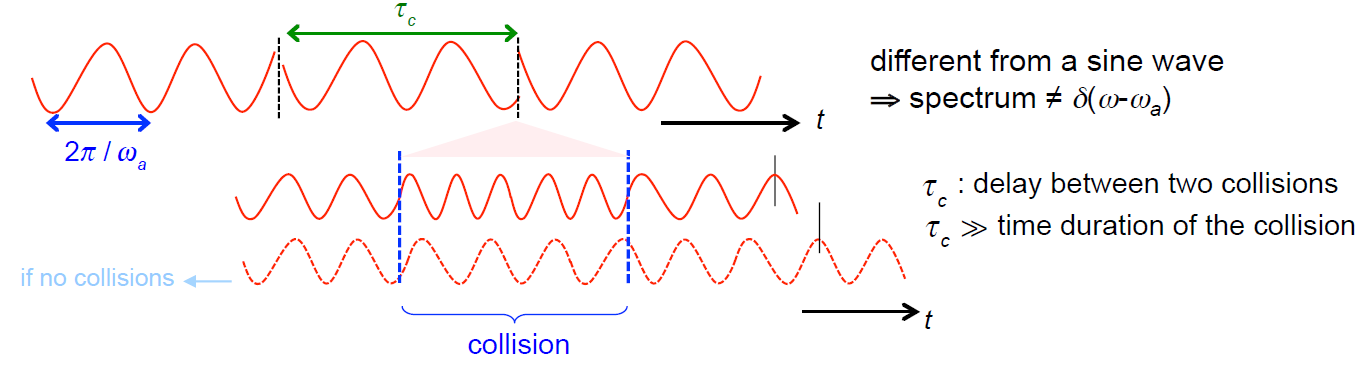
\includegraphics[width=0.7\textwidth,height=10\baselineskip,keepaspectratio]{ch3/image20} 
	\caption{Désiquilibre parallèle: garde} 
\end{figure}
\subsection{Montage différentiel avec \texorpdfstring{\(v_{mc}\)}{tension de mode commun} élevée}\label{subsec:montdiffvmcgrand}
Avant, on avait \(2N+1\) conducteurs et un \(v_{mc}\) relativement faible (les 2 références restaient proches). Dans le cas d'un source flottante (pas connectée à la référence) on a:
\begin{itemize}
	\item \(2N\) conducteurs
	\item tension de mode commun quelconque et variable dans le temps (AC + DC)
\end{itemize}
Une très mauvaise idée car nous avons une source de perturbations importante qui risque de détruite le matériel par surtension.

N.B.: vérifier la capa de l'ampli à tenir la tension de mode commun (\!?).
\subsubsection{1\up{ère} solution: bias resistor pour source flottante}
Il faut limiter la tension de mode commun, donc soit on utilise \(2N+1\) conducteurs (donc retour au cas précédent) soit on utilise des résistances offrant une liaison galvanique de haute impédance ("bias resistor):
\begin{itemize}
	\item meilleur symétrie que \(2N+1\) conducteurs
	\item valeur suffisamment élevée pour ne pas imposer le potentiel des entrées
	\item mais suffisamment faible pour éviter que la tension de mode commun soit trop éloignée de la référence de l’instrumentation
	\item typiquement: \SI{10}{\kilo\ohm} à \SI{100}{\kilo\ohm}
\end{itemize}
\begin{figure}[H] 
	\centering 
	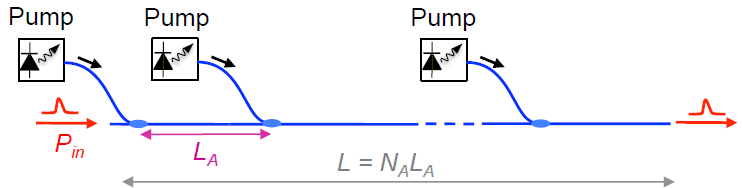
\includegraphics[width=0.7\textwidth,height=10\baselineskip,keepaspectratio]{ch3/image21} 
	\caption{bias resistor pour source flottante} 
\end{figure}
\subsubsection{2\up{ème} solution: ampli d'isolation}
\begin{figure}[H] 
	\centering 
	\includegraphics[width=0.7\textwidth,height=10\baselineskip,keepaspectratio]{ch3/image22} 
	\caption{Ampli d'isolation} 
\end{figure}
Comme ceci l'instrumentation au potentiel du capteur possède sa propre alimentation et donc pas de mode commun.
\subsection{Conclusion}
Il y a 3 cas à distinguer:
\begin{enumerate}
	\item les références sont identiques:
	\begin{itemize}
		\item différence de potentiel nulle ou négligeable: c'est l'exception, les f.e.m. par impédance de masse et parasites sont négligeables, la référence est indifféremment la masse ou la terre. Un simple montage asymétrique convient.
	\end{itemize}
	\item les références sont proches:
	\begin{itemize}
		\item tension de mode commun "faible": typiquement un cas \(2N+1\) fils. Un montage différentiel "simple" convient (il faut vérifier la limite de l'ampli vis-à-vis du mode commun)
	\end{itemize}
	\item les références sont éloignées:
	\begin{itemize}
		\item tension de mode commun élevée (ou quelconque): capteur flottant et porté à un potentiel élevé. Il faut limiter le mode commun \(\Rightarrow 2N+1\) fil ou bias resistors ou reprendre le mode commun grâce à l'ampli d'isolation.
	\end{itemize}
\end{enumerate}
De plus, au niveau de la boucle différentielle, les mesures classiques pour limiter les parasites sont le câble torsadé ou coaxial, le blindage des câbles (complexe), etc.
\section{Transmission des signaux}
\subsection{Introduction}
La majorité des transmissions des signaux se font par tension analogique, le montage différentiel ne résout pas tout (il résout surtout le couplage galvanique). Pour les environnements très parasités et/ou longues distances, nous aurons recours à des transmissions par boucle de courant, par fréquence, par signal optique ou des transmission numérique.
\subsubsection{Inconvénients d'une transmission en tension}
Illustrons une transmission en tension (\autoref{fig:transmtension}). Nous aurons donc \(R_{in}\) élevé et \(R_{out}\) faible (adaptation d'impédance en tension) mais la liaison à distance possède une \(R_{\text{fils}}\) non négligeable. La sortie obtenue est donc 
\[v = e\frac{R_{in}}{R_{out}+R_{in}+R_{\text{fils}}}<e\]
On a donc un affaiblissement du signal, 1\up{er} inconvénient.\\
Prenons le cas maintenant d'une tension parasite par couplage magnétique (\autoref{fig:transmtensionpara})
\[v = (e_s+e_p)\frac{R_{in}}{R_{out}+R_{in}}\]
Le parasite induit se superpose au signal, 2\up{ème} inconvénient
\begin{figure}[H] 
	\centering 
	\includegraphics[width=0.6\textwidth,height=10\baselineskip,keepaspectratio]{ch3/image23} 
	\caption{Transmission en tension: résistance de ligne} 
	\label{fig:transmtension}
\end{figure}
\begin{figure}[H] 
	\centering 
	\includegraphics[width=0.6\textwidth,height=10\baselineskip,keepaspectratio]{ch3/image24} 
	\caption{Transmission en tension: parasite de ligne par couplage magnétique} 
	\label{fig:transmtensionpara}
\end{figure}
\subsection{Boucle de courant}
Le but est de passer l'information non plus par une tension, mais par un courant. Il est en pratique plus facile d'obtenir \(R_{out}\) (commande en courant) élevée que \(R_{in}\) élevée (commande en tension). Dans le cas de la \autoref{fig:transcourant}, nous obtenons \((R_{in}+R_{fils})i = R_{out}(i_s-i)\) et donc
\[i=\frac{R_{out}}{R_{out}+R_{in}+R_{fils}}i_s\]
L'affaiblissement du signal est beaucoup plus faible qu'en tension (car plus facile d'obtenir un \(R_{out}\) élevée qu'un \(R_{in}\) élevée).\\
Avec le couplage magnétique (\autoref{fig:transcourantpara}):
\[i_p=\frac{e_p}{R_{out}+R_{in}}\]
Comme \(R_{out}\) élevée, \(i_p\ll i_s \Rightarrow\) bonne immunité aux parasites magnétiques.\\
Plusieurs avantages:
\begin{itemize}
	\item bien pour transmission longue distance (\SI{1}{\kilo\meter} ou plus) car l'impédance des fils influence peu le courant
	\item bonne immunité aux f.e.m. induites car les valeurs idéales de \(R_{out}\text{ et }R_{in}\) sont plus facile à approcher en commande en courant qu'en commande en tension
	\item On peut utiliser un courant \(\neq0\) pour représenter la valeur 0 afin de détecter la rupture de la liaison
\end{itemize}
\begin{figure}[H] 
	\centering 
	\includegraphics[width=0.6\textwidth,height=10\baselineskip,keepaspectratio]{ch3/image35} 
	\caption{Transmission en courant: résistance de ligne} 
	\label{fig:transcourant}
\end{figure}
\begin{figure}[H] 
	\centering 
	\includegraphics[width=0.6\textwidth,height=10\baselineskip,keepaspectratio]{ch3/image36} 
	\caption{Transmission en courant: parasite de ligne par couplage magnétique} 
	\label{fig:transcourantpara}
\end{figure}
\section{Câblage de la masse}
On a plusieurs circuits qui partagent la même alimentation et qui doivent s'échanger de l'information, chacun devant être connecté à une référence unique (masse). Comment câbler?
\subsection{Interconnexion des circuits}
Il faut éviter les impédances communes \(\rightarrow\) mettre en étoile \(\rightarrow\) si le PCM à une impédance nulle \(\Rightarrow\) pas de couplage d'impédance
\begin{figure}[H] 
	\centering 
	\includegraphics[width=0.8\textwidth,height=10\baselineskip,keepaspectratio]{ch3/image25} 
	\caption{Interconnexion des circuits en étoile} 
\end{figure} 
\subsection{Câblage de la masse analogique}
\begin{figure}[H] 
	\centering 
	\includegraphics[width=0.6\textwidth,height=10\baselineskip,keepaspectratio]{ch3/image26}
\end{figure}
Dans le cas analogique, que faire ? Étoile ou cascade ?
\subsubsection{Masse en étoile}
\begin{figure}[H] 
	\centering 
	\includegraphics[width=0.8\textwidth,height=10\baselineskip,keepaspectratio]{ch3/image27} 
	\caption{Masse analogique en étoile} 
\end{figure}
\begin{description}
	\item[Avantages] pas d'impédance commune
	\item[Désavantages] longueur des pistes et formation de boucle
\end{description}
\subsubsection{Masse en cascade}
\begin{figure}[H] 
	\centering 
	\includegraphics[width=0.8\textwidth,height=10\baselineskip,keepaspectratio]{ch3/image28} 
	\caption{Masse analogique en cascade (amont)} 
\end{figure}
Dans ce cas-ci, tous les courants passent pas \(R_1 \Rightarrow V_{in}=V_{out}/\num{e4}\) car on amplifie \(V_{in}+ i_iR_1\)!
\begin{figure}[H] 
	\centering 
	\includegraphics[width=0.8\textwidth,height=10\baselineskip,keepaspectratio]{ch3/image29} 
	\caption{Masse analogique en cascade (aval)} 
\end{figure}
Dans ce cas-là, nous avons minimiser les courants dans \(R_1\).
\subsection{Câblage de la masse numérique}
À haute fréquence, l'effet selfique des câbles devient dominant \(\Rightarrow\) pistes à grande impédance et courants passent par capas parasites\(\Rightarrow\) \cancel{masse en étoile} plan de masse (minimise les inductances et les boucles). Le courant suivra le chemin de moindre impédance.
\begin{figure}[H] 
	\centering 
	\includegraphics[width=0.5\textwidth,height=10\baselineskip,keepaspectratio]{ch3/image30} 
	\caption{Plan de masse} 
\end{figure}
\subsection{CAN et CNA}
\begin{figure}[H] 
	\centering 
	\includegraphics[width=0.5\textwidth]{ch3/image31} 
\end{figure}
Dans un CAN/CNA, il y a un faible courant qui circule à travers sa capa parasite.\\
Il faut 2 masses distinctes pour conserver une topologie en étoile et il faut placer le CAN sur le point central de masse
\begin{figure}[H] 
	\centering 
	\includegraphics[width=0.7\textwidth,height=10\baselineskip,keepaspectratio]{ch3/image32} 
\end{figure}
\subsubsection{Câblage des alimentation}
2 problèmes se posent:
\begin{itemize}
	\item Ripple des alimentation à découpage (fluctuation autour de la valeur consigne)
	\item Consommation des différents circuits
\end{itemize}
\begin{figure}[H] 
	\centering 
	\includegraphics[width=0.7\textwidth,height=10\baselineskip,keepaspectratio]{ch3/image33}  
\end{figure}
Il faut mettre une capa a côté du composant, elle jouera le rôle de réservoir de charge. Sachant que la résistance parasite est d'autant plus grande que la capa est grande, on placera une plus petite capa en parallèle dans le cas HF car c'est la résistance qui est gênante.
\begin{figure}[H] 
	\centering 
	\includegraphics[width=0.6\textwidth,height=10\baselineskip,keepaspectratio]{ch3/image34}  
\end{figure}
%\chapter{Light Propagation in Linear Anisotropic Dielectrics}
\textit{"C'est mon chapitre préféré, celui que j'ai choisi lorsque j'étais à votre place. Ne ne négligez pas!}

\section{Anisotropic Materials in Photonics}
Beaucoup de matériaux ont des propriétés optiques quid épendent de la direction de la lumière ou de sa polarisation. 
Notons que dans un polariseur, si les polymères sont étendus en $y$, l'onde qui passera sera en $x$ !

\section{The Susceptibility and Dielectric Tensors}
\subsection{Constitutive Equations in Anisotropic Media}
	\begin{wrapfigure}[8]{l}{8cm}
	%\vspace{-5mm}
	\includegraphics[scale=0.4]{ch4/image1.png}
	\captionof{figure}{ }
	\end{wrapfigure}
Lorsque le matériau n'est pas isotrope, $\vec{P}$ n'est pas toujours parallèle à $\vec{E}$ : la polarisation va
dépendre de la direction du champ électrique. Si dans une direction nous avons $n_1$ et dans une autre $n_2$ 
avec $n_a<n_b$, la superposition des deux donnera une polarisation non parallèle au champ appliqué. \\

La relation linéaire la plus générale entre deux vecteurs est un tenseur du second rang. Dès lors
\begin{equation}
P = \epsilon_0\overline{\overline{\chi}}E\qquad\text{ou}\qquad P_i = \epsilon_0\chi_{ij}E_j
\end{equation}
où $\overline{\overline{\chi}}$ est le \textbf{tenseur de susceptibilité}. S'il est diagonal avec tout des 
coefficients identiques, on se retrouve au cas du chapitre 2. Mais si non, la polarisation induite peut dépendre
de la direction de $\vec{E}$.

\subsection{Symmetry of the Susceptibility Tensor}
Il est simple de montrer analytiquement que le tenseur de susceptibilité est symétrique (sous certaines conditions).
Soit le théorème de Poynting
\begin{equation}
\dfrac{\partial U}{\partial t} = -\nabla.S-EJ_p
\end{equation}
où $U$ est la densité d'énergie EM et $\vec{S}$ le vecteur de Poynting
\begin{equation}
U = \frac{1}{2}\epsilon_0\left(|E|^2-c^2|B|^2\right),\qquad\qquad
S \equiv \left\langle \vec{E}\times\vec{H}\right\rangle = \frac{1}{\mu_0}
\left\langle \vec{E}\times\vec{B}\right\rangle
\end{equation}
Comme il  n'y a pas de courants libre, de magnétisation, le milieu est transparent et non-dissipant, l'énergie
n'est pas convertie en chaleur. L'énergie du champ peut aller dans la matière, mais elle sera "rendue" au final.
Il doit donc être possible de noter le troisième terme sous la forme d'une dérivée temporelle ou d'une divergence
afin de la faire passer dans le membre de gauche.\\

Dans la convention d'Einstein
\begin{equation}
E_kJ_{p,k} = E_k\frac{\partial P_k}{\partial t} = \frac{1}{2}E_k\epsilon_0\chi_{kl}\frac{\partial E_l}{\partial t}+
\frac{1}{2}E_l\epsilon_0\chi_{lk}\frac{\partial E_k}{\partial t}
\end{equation}
On peut toujours écrire $\chi_{kl} = \chi_{kl}^S+\chi_{kl}^A$. Il nous faudra montrer que $\chi_{kl}^A$ est
nulle. Le terme source devient\footnote{Voir page 62 pour le détail}
\begin{equation}
E_kJ_{p,k} = \frac{1}{2}\epsilon_0\chi_{kl}^S\frac{\partial (E_kE_l)}{\partial t}+\frac{1}{2}
\epsilon_0\chi_{kl}^A\left(E_k\frac{\partial E_l}{\partial t}-E_l\frac{\partial E_k}{\partial t}\right)
\end{equation}
Seule la partie symétrique peut s'écrire sous la forme d'une dérivée temporelle, la partie antisymétrique doit
forcément être nulle. Poynting s'écrit alors
\begin{equation}
\dfrac{\partial U_{total}}{\partial t}= -\nabla S
\end{equation}
où $U_{total}$ est la densité d'énergie totale
\begin{equation}
U_{total} = \frac{1}{2}D.E+\frac{1}{2}B.H
\end{equation}
Ceci n'est vrai que pour les matériaux non magnétique et non-dispersif.


\section{Plane Monochromatic Waves in Anisotropic Media}
\subsection{Dispersion Relation}
Nous allons ici analyser sir les ondes planes monochromatiques sont toujours solutions des équations de 
Maxwell et des équations constitutives (soit les équations de l’électrodynamique). Nous avons\footnote{Détails
page 63}
\begin{equation}
\nabla\times\left(\nabla\times\vec{E}\right) = -\frac{1}{c^2}\dfrac{\overline{\overline{\epsilon}}}{\epsilon_0}
\frac{\partial^2E}{\partial t^2}
\label{eq:4.41}
\end{equation}
C'est difficile, mais il existe un système de coordonnées ou ce tenseur est diagonal : tout va devenir "simple"
\footnote{Résultat attendu : le tenseur $\epsilon$ doit être symétrique, il doit exister une base où il est
diagonal}. Dans un tel système, le tenseur diélectrique est donné par (semble trivial, mais en réalité profond)
\begin{equation}
\dfrac{\overline{\overline{\epsilon}}}{\epsilon_0} =\left(\begin{array}{ccc}
n_1^2 & 0 &0\\
0 &n_2^2 &0\\
0&0&n_3^2
\end{array}\right)
\end{equation}
où $n_i$ sont les indices de réfraction principaux. L'équation \eqref{eq:4.41} devient quelque chose de 
"\textit{pas si moche}" : 
\begin{equation}
\vec\nabla\times(\vec\nabla\times\vec E) = -\frac{1}{c^2}\left(\vec{1_x} n_1^2\dfrac{\partial^2 E_x}{\partial t^2}
+\vec{1_y} n_2^2\dfrac{\partial^2 E_y}{\partial t^2}+\vec{1_z} n_3^2\dfrac{\partial^2 E_z}{\partial t^2}\right)
\end{equation}
On veut trouver une relation de dispersion $\omega(k)$. On propose une solution d'onde plane monochromatique 
de pulsation $\omega$ et de vecteur d'onde $\vec{k}$ à cette équation différentielle
\begin{equation}
E = E_0e^{i(\omega t-k.r)}
\end{equation}
En substituant cet ansat, on trouve (rot $\to\ ik$)
\begin{equation}
i\vec k\times(i\vec k\times \vec E_0) = \frac{\omega^2}{c^2}\left(\vec 1_x n_1^ 2 E_{0x}+
\vec 1_y n_2^ 2 E_{0y}+\vec 1_z n_3^ 2 E_{0z}\right)
\end{equation}
Sachant que $\vec A\times(\vec B\times \vec C) = -(\vec A\vec B)\vec C+(\vec A\vec C)\vec B$ 
\begin{equation}
\vec k(\vec k . \vec E_0) - \vec E_0 k^2 = -\frac{\omega^2}{c^2}\left(\vec 1_x n_1^ 2 E_{0x}+
\vec 1_y n_2^ 2 E_{0y}+\vec 1_z n_3^ 2 E_{0z}\right)
\end{equation}
Il s'agit de la relation de dispersion pour un milieu linéaire non isentropique. En projetant cette équation 
sur les axes principaux (par exemple sur $\vec 1_x$ on a : $k_x \vec 1_x \left(k_x E_{0x} + k_y E_{0y} + k_z E_{0z}\right) - E_{0x} \vec 1_x\left(k_xk_x + k_y k_y + k_z k_z\right) =
-\frac{\omega^2}{c^2} \vec 1_x n_1^2 E_{0x}$) on voit que la relation de dispersion est un système linéaire
en les trois composantes du champ électrique
\begin{equation}
\left(\begin{array}{ccc}
\frac{\omega^2}{c^2}n_1^2-k_y^2k_z^2 & k_xk_y & k_xk_z\\
k_yk_x & \frac{\omega^2}{c^2}n_2^2-k_x^2-k_z^2 & k_yk_z\\
k_zk_x & k_zk_y & \frac{\omega^2}{c^2}n_3^2-k_x^2-k_y^2
\end{array}\right)\left(\begin{array}{c}
E_{0x}\\
E_{0y}\\
E_{0z}
\end{array}\right) = 0
\label{eq:4.19}
\end{equation}



\subsection{The Normal Surface}
Considérons d'abord quelques situations simplifiées
\begin{enumerate}
\item Vecteur d'onde parallèle à $\vec{1_x}$ : $k_x=k$. Le système \eqref{eq:4.19} se réduit à 
\begin{equation}
\left\{\begin{array}{rl}
\DS\frac{\omega^ 2}{c^2}n_1^2 E_{0x} &= 0\vspace{2mm}\\
\DS\left(\frac{\omega^2}{c^2}n_2^2-k^2\right)E_{0y}&=0\vspace{2mm}\\
\DS\left(\frac{\omega^2}{c^2}n_3^2-k^2\right)E_{0z}&=0
\end{array}\right.
\end{equation}
La première équation nous informe que le champ est transverse et les deux dernières les solutions : si les $E_{0i}$
sont non-nuls, la parenthèse doit l'être : on en tire les relations de dispersions.La première est l'onde plane
polarisée selon $y$ de nombre d'onde $k_2$
\begin{equation}
E^{(1)} = \vec{1_y}E_0^{(1)}e^{i(\omega t-k_2x)}\qquad\text{ où }\quad k_2 = \frac{\omega}{c}n_2
\end{equation}
La seconde est l'onde plane polarisée selon $z$ de nombre d'onde $k_3$
\begin{equation}
E^{(2)} = \vec{1_z}E_0^{(2)}e^{i(\omega t-k_3x)}\qquad\text{ où }\quad k_3 = \frac{\omega}{c}n_3
\end{equation}
\end{enumerate}






%\chapter{Cinétique du réacteur ponctuel}
\section{Équation de cinétique ponctuelle}
\subsection{Introduction}
Nous avons eu du mal avec six variables, ça risque d'être pire si on ajoute le temps. Si il était 
possible de faire une sorte de séparation des variables, ça pourrait bien se simplifier
\begin{equation}
\varphi (\bar r,v,\bar \Omega ,t)\, \equiv \;T(t).\psi (\bar r,v,\bar \Omega )
\end{equation}
Ceci suppose que s'il y a des variations dans le temps la forme reste inchangée mais l'amplitude 
varie au cours du temps.  Hélas, ceci n'est possible que si $J,K$ sont constants ce qui n'est pas
réaliste. Cependant, une "fausse factorisation" peut être acceptable dans le cas où les perturbations 
n'affectent que peu la forme du flux autour de la criticité (une sorte de transitoire)
\begin{equation}
\varphi (\bar r,v,\bar \Omega ,t)\, \equiv \;T(t).\psi (\bar r,v,\bar \Omega ,t)
\end{equation}
où $T(t)$ est une fonction d'amplitude qui reprend les variations dépendantes du temps sur des temps
caractéristiques courts. Il y aura également une variation temporelle de $\psi$, mais plus lente. En 
bref, très rapidement on aura un facteur de multiplication du flux et puis, plus lentement, des 
changements dans le réacteur. Les barres avaleuses de neutrons correspondent à une telle situation.\\

Le raisonnement est le suivant
\begin{enumerate}
\item On utilise la factorisation \textit{partielle} $\varphi (\bar r,v,\bar \Omega ,t)\, \equiv \;T(t).
\psi (\bar r,v,\bar \Omega ,t)$  dans l'équation de Boltzmann avec les neutrons retardés (évidemment 
car ils dépendent du temps)(sans oublier la normalisation)
\item On regarde l'impact des hypothèses d'une factorisation \textit{exacte} $\varphi (\bar r,v,\bar \Omega ,t)\, \equiv \;T(t).\psi (\bar r,v,\bar \Omega )$
\begin{itemize}
\item[$\bullet$] Déduction d'un modèle d'évolution du réacteur sujet à des perturbations autour de
l'état stationnaire critique de régime
\item[$\bullet$] Solution exacte et approximée en fonction du type de perturbation
\end{itemize}
\end{enumerate}

\subsection{Déduction intuitive des équations ponctuelles}
\subsubsection{Évolution de la population neutronique sans neutrons et sources retardées}
Commençons par un peu d'intuition. Nous avions vu, au premier chapitre
\begin{equation}
\frac{{dN(t)}}{{dt}} = \frac{{{k_{eff}} - 1}}{\ell }N(t)
\end{equation}
où $l$ est la durée moyenne sur laquelle les neutrons sont consommés dans un cycle : nous avions 
un trop plein de neutrons qui donnait une ED avec une solution exponentielle ingérable, il était 
nécessaire d'introduire les neutrons retardés.\\

Considérons une fonction amplitude $T$ ($\propto N$) des neutrons retardés ainsi qu'une source 
indépendante
\begin{equation}
\frac{{dT(t)}}{{dt}} = \frac{{{k_{eff}}(1 - \beta ) - 1}}{\ell }T(t) + \sum\limits_{i = 1}^6    {\lambda _i}{c_i}(t) + q(t)
\end{equation}
où $c_i(t)$ est la concentration en précurseurs du groupe $i$. Le $(1-\beta)$ donne la fraction des neutrons prompts, le $-1$ l'éventuel surplus puis pomme il faut exprimer par cycle on divise par $l$
et on multiplie le tout par $T$. \\

Introduisons un autre temps caractéristique $\Lambda$ lié au $k_{eff}$ tel que $l=\Lambda k_{eff}$ 
ainsi que la \textbf{réactivité}, l'écart relatif de distance à la criticité
\begin{equation}
\rho  \equiv \frac{{{k_{eff}} - 1}}{{{k_{eff}}}}
\end{equation}
En substituant\footnote{Besoin de notes manuscrites}, on trouve
\begin{equation}
\frac{{dT(t)}}{{dt}} = \frac{{\rho  - \beta }}{\Lambda }T(t) + \sum\limits_{i = 1}^6   {\lambda _i}{c_i}(t) + q(t)
\end{equation}
Le seuil \textit{prompt-critique}\footnote{Notes manuscrites!} correspond au cas où la criticité est
obtenue \textbf{uniquement} avec des neutrons prompts soit le cas où $k_{eff}=(1-\beta)^{-1}$. En 
en tire
\begin{equation}
\rho = \beta
\end{equation}
En l'exprime en \%, pcm où en \$ (1\$ si $\rho = \beta$). \\

Tentons d'interpréter le temps caractéristique dans le cas mono-cinétique. On se rappelle que 
$\Sigma_a$ est la probabilité par unité de longueur d'avoir une interaction dans le libre 
parcours. Si on multiplie ce-dernier par la vitesse $v$, on aura la probabilité par unité de temps
d'avoir une absorption. Le temps moyen est bien l'inverse de cette grandeur et porte le nom de 
\textbf{temps de destruction}
\begin{equation}
\ell  = \frac{1}{{v{\Sigma _a}}}
\end{equation}
De façon similaire, $\frac{1}{v\Sigma_f}$ est le temps moyen pour avoir une fission. Si on divise 
ceci par le nombre de neutrons $\nu$, on trouve le temps moyen que met un neutron pour générer une 
fission, soit le \textbf{temps de production}
\begin{equation}
\Lambda  = \frac{1}{{\nu v{\Sigma _f}}}
\end{equation}
La criticité est atteinte si et seulement si $\Lambda=l$.


\subsection{Modèle du réacteur ponctuel}
Reprenons notre fonction amplitude
\begin{equation}
\frac{{dT(t)}}{{dt}} = \frac{{\rho \;\;\; - \beta }}{\Lambda }T(t) + \sum\limits_{i = 1}^6   {\lambda _i}{c_i}(t) + q(t)
\end{equation}
La concentration en précurseurs dans le groupe $i$ est donnée par
\begin{equation}
\frac{{d{c_i}(t)}}{{dt}} = \frac{{{\beta _i}}}{\Lambda }T(t) - {\lambda _i}{c_i}(t)
\end{equation}
Cette variation est constituée d'une diminution radioactive des précurseurs et d'une fraction 
$\beta_i$ qui se rajoute à cette concentration par cycle (on a bien une division par le temps de
production des neutrons): chaque fois que l'on a une contribution au flux, il y a une fraction
$\beta_i$ qui correspond aux neutrons retardés et donc les précurseurs du groupe correspondant 
(fragments). Ceci nous donne un système de $6+1=7$ équations. \\

Les variations de $T$ sont dues à des variations du flux causée par des variations de la puissance 
et donc des variations de températures. Nous avions jusqu'ici supposé que la vitesse des noyaux 
lourds était négligeable mais s'il y a une variation de la température du réacteur on va avoir une
nuance entre la vitesse absolue et relatives des neutrons et des noyaux lourds avec lesquels ils 
interagissent. Une variation de $T$ cause donc une variation de l'équation générale du réacteur car 
modifier le température de l'eau modifie sa densité impliquant un ralentissement des neutrons plus
ou moins important. \\

Tout ceci pour dire que $T$ varie, on aura un effet sur la réactivité (car écart par rapport à 
l'équilibre). Le problème devient linéaire et pour tenir compte de ceci un suppose une réactivité
dépendante du temps mais extérieure\footnote{On néglige la rétroaction et on voit $\rho(t)$ comme 
un signal extérieur.} : $\rho\to\rho(t)$.

\subsection{Solution des équations cinétiques ponctuelles pour une marche de réactivité}
\subsubsection{Problématique}
On s'intéresse au déplacement rapide en $t=0$ des barres de commande dans un réacteur initialement
stable et critique sans source
\begin{equation}
\left\{ {\begin{array}{*{20}{c}}
{\rho (t) = 0}&{,\;t < 0}\\
{\rho (t) = \rho }&{,\;t \ge 0}
\end{array}} \right.
\end{equation}
Il faut résoudre nous deux équations différentielles de $\dot{T}$ et $\dot{c}$. En effectuant 
la transformée de Laplace\footnote{Notes manuscrites!}
\begin{equation}
\left\{\begin{array}{ll}
\bar T(p) &\DS= \frac{{\Lambda (T(0) + \sum\nolimits_i    {\textstyle{{{\lambda _i}{c_i}(0)} \over {p + {\lambda _i}}}})}}{{\Lambda p - \rho  + \sum\nolimits_i    {\textstyle{{{\beta _i}p} \over {p + {\lambda _i}}}}}}\\
{\bar c_i}(p) &\DS= \frac{{{\textstyle{{{\beta _i}} \over \Lambda }}\bar T(p) + {c_i}(0)}}{{p + {\lambda _i}}}
\end{array}\right.
\end{equation}
Avec comme $\DS CI\; \to \;\left( {{\lambda _i}{c_i}(0) = \frac{{{\beta _i}}}{\Lambda }T(0)} \right)$. 
Introduisons une fonction $1/G$ car on retrouve celle-ci de chaque côté de l'égalité à $p$ près\footnote{Il faudrait des notes pour éclaircir ces opérations}
\begin{equation}
{[G(p)]^{ - 1}} \equiv p\left(   \right.1 + \frac{1}{\Lambda }\sum\limits_i    \frac{{{\beta _i}}}{{p + {\lambda _i}}}\left.    \right)
\end{equation}
Ce qui permet d'écrire\\
	\begin{wrapfigure}[5]{l}{5cm}
	\vspace{-5mm}
	\includegraphics[scale=0.23]{ch5/image1.png}
	\captionof{figure}{ }
	\end{wrapfigure}
\cadre{
\begin{equation}
\frac{{\bar T(p)}}{{T(0)}} = \frac{1}{{p[1 - {\textstyle{\rho  \over \Lambda }}G(p)]}}
\end{equation}}\ \\

Il s'agit d'une expression donnant sept pôles possibles. Le pôle dominant donne le comportement 
dominant. Pour $\rho >0$ le pôle dominant est positif alors qu'il est négatif pour $\rho<0$.\vspace{3mm}


\subsubsection{Inversion de $\bar T(p)$}
Identifions les pôles, soit les racines de $\rho =\dfrac{\Lambda}{G(p)}$. Notons que $p=0$ n'est 
pas un pôle s'il n'y a pas de source. Nous avions vu avec l'illustration ci-dessus qu'il y avait
sept pôles
\begin{itemize}
\item[$\bullet$] $\rho<0$ : 7 pôles.
\item[$\bullet$] $\rho>0$ : 6 pôles négatif et un positif $\to p_0>0>p_1>\dots > p_6$.
\end{itemize}\ 

Tout dans ce problème est connu, par calcul des résidus il est possible de calculer les valeurs 
exactes des écarts. Dans notre cas, on s'intéresse au pôle qui a la plus grande valeur (le plus loin
sur l'axe $p$) car l'inverse de ce pôle en valeur absolue donnera le temps caractéristique 
apparaissant dans l'exponentielle dominante (comportement en $e^{\pm t/\tau)}$ que le réacteur va
suivre pour cet échelon de réactivité
\begin{equation}
T(t) = \sum\limits_{k = 0}^6    {T_k}{e^{{p_k}t}}\quad\overset{t\to\infty}{\longrightarrow}\quad {T_o}{e^{{p_o}t}}
\end{equation}
où $\DS \frac{{{T_k}}}{{T(0)}} = \mathop {\lim }\limits_{p \to {p_k}} \frac{{p - {p_k}}}{{p[1 - {\textstyle{\rho  \over \Lambda }}G(p)]}} = \frac{1}{{1 - {\textstyle{\rho  \over \Lambda }}(G({p_k}) + {p_k}G'({p_k}))}}  = \frac{{1 + \frac{1}{\Lambda }\sum\limits_i    \frac{{{\beta _i}}}{{{p_k} + {\lambda _i}}}}}{{1 + \frac{1}{\Lambda }\sum\limits_i   \frac{{{\beta _i}{\lambda _i}}}{{{{({p_k} + {\lambda _i})}^2}}}}}$.\\

La période asymptotique du réacteur est donc donnée par $\tau = 1/|p_0|$. On en tire une relation
\textit{période-réactivité} qui porte le doux nom d'\textbf{équation inhour}\\

\cadre{\begin{equation}
\rho  = \frac{\Lambda }{{G(1/\tau )}}
\end{equation}}\ \\

A l'aide de cette équation, il est possible en mesurant le temps nécessaire $\tau$ pour une variation
du flux d'en déduire $\rho$, par exemple liée à la descente des barres de contrôles d'un coup dans 
le réacteur. Il s'agit du temps nécessaire pour que le flux varie d'un facteur $e$ en croissance ou en
décroissance selon le signe de la réactivité.

\subsubsection{Cas limites}
Reprenons l'équation inhour en écrivant celle-ci par rapport à la période et non plus par rapport 
à $p$
\begin{equation}
\rho  \equiv \frac{\Lambda }{\tau }\left(    1 + \frac{1}{\Lambda }\sum\limits_i    \frac{{{\beta _i}\tau }}{{1 + {\lambda _i}\tau }}    \right)
\end{equation}
En se rappelant que $\beta$ est le seuil prompt-critique, voyons trois cas limites
\begin{enumerate}
\item \textit{Grande réactivité} : $\rho > \beta \to \lambda_i\tau \ll 1$. Ceci signifie que la 
période est très petite par rapport au $1/\lambda_i$ soit le temps de vie des précurseurs : les
$\lambda_i\tau$ peuvent être négligés dans l'équation inhour
\begin{equation}
\rho  \equiv \frac{\Lambda }{\tau }\left(   1 + \frac{1}{\Lambda }\sum\limits_i    \frac{{{\beta _i}\tau }}{{1 + {\lambda _i}\tau }}    \right)\overset{\lambda_i\tau\ll 1}{\longrightarrow}  \frac{\Lambda }{\tau } + \beta \qquad\Rightarrow\qquad \tau\longrightarrow \frac{\Lambda }{{\rho  - \beta }}
\end{equation}
Le temps ne dépend en aucune manière des $\lambda_i$ (invese des temps caractéristiques des neutrons
retardés). Ainsi, au dessus du seuil prompt-critique, la période asymptotique dépend de $\Lambda$ mais
(encore une fois) pas des $1/\lambda_i$ qui sont lié (à $\ln 2$ près) à la demi-vie des précurseurs. 
L'agrandissement du flux $\varphi$ est trop rapide pour que les neutrons retardés puissent jouer un rôle au dessus du seuil prompt-critique donné par $k_{eff}(1-\beta)=1$.

\item \textit{Petite réactivité} : $0<\rho\ll \beta \to \lambda_i\tau \gg 1$. Ceci signifie que 
$\rho$ se rapproche à l'horizontale à zéro et donc la valeur du pôle dominant est petite impliquant
une période grande.  Avec cette approximation, c'est le 1 dans le dénominateur de l'équation inhour 
que l'on négliger. Cette simplification permet de simplifier les $\tau$ dans la fraction
\begin{equation}
\rho  \equiv \frac{\Lambda }{\tau }\left(    1 + \frac{1}{\Lambda }\sum\limits_i    \frac{{{\beta _i}\tau }}{{1 + {\lambda _i}\tau }}    \right)\overset{\lambda_i\tau\gg1}{\longrightarrow}  \frac{1}{\tau }(\Lambda  + \beta \bar \tau )
\end{equation}
Comme précédemment, $1/\lambda_i$ est le temps de demi-vie des précurseur : on fait apparaître un 
temps moyen $\bar\tau$ car la sommation ne faut que pondérer les $1/\lambda_i$ par $\beta_i/\beta$.
\begin{equation}
\bar \tau  \equiv \sum\limits_i    \frac{{{\beta _i}/\beta }}{{{\lambda _i}}}
\end{equation}
Il s'agit donc du temps de vie moyen des neutrons retardés pondéré par leur fraction relative. Notons
que cette expression est indépendante de $\Lambda$. Ici, ce sont les neutrons retardés qui commandent
la croissance du flux $\varphi$ comme nous l'avions déduit intuitivement au premier chapitre. 

\item \textit{Réactivité <0}. Il y a un pôle dominant entre 0 et $\lambda_1$ qui est le pôle le plus
petit en valeur absolue. La période est plus grande que le temps caractéristique le plus grand des 
demi-vie des neutrons retardés, il en résulte un écrasement de la valeur du flux liée au temps 
caractéristique des neutrons retardés
\begin{equation}
\tau  > 1/{\lambda _1}
\end{equation}
\end{enumerate}


\subsubsection{Modèle ponctuel à un groupe de neutrons retardés}
Nos deux équations à résoudre sont
\begin{equation}
\frac{{dT(t)}}{{dt}} = \frac{{\rho (t) - \beta }}{\Lambda }T(t) + \lambda c(t),\qquad\qquad
\frac{{dc(t)}}{{dt}} = \frac{\beta }{\Lambda }T(t) - \lambda c(t)
\end{equation}
En dérivant $dT/dt$ on fait apparaître $dc/dt$ et on peut y substituer la seconde équation\footnote{Notes manuscrites!!}. On se retrouve alors avec une équation qui où n'apparaît que $T$. En 
faisant la résolution de cette équation (solutions exponentielles ou partir de l'équation inhour 
à un seul groupe) on trouve une équation du second degré en $p$ donnant les pôles
\begin{equation}
\rho  \equiv \Lambda p\left(   \right.1 + \frac{1}{\Lambda }\frac{\beta }{{p + \lambda }}\left.    \right)
\end{equation}
Après résolution 
\begin{equation}
\left. {\begin{array}{*{20}{c}}
{{\omega _1}}\\
{{\omega _2}}
\end{array}} \right\} =  - \frac{{\beta  - \rho  + \lambda \Lambda  \pm \sqrt {{{(\beta  - \rho  + \lambda \Lambda )}^2} + 4\lambda \Lambda \rho } }}{{2\Lambda }}\quad\overset{{\lambda \Lambda  \ll \beta  - \rho }}{\longrightarrow} \quad
\left\{ {\begin{array}{*{20}{c}}
\DS{{\omega _1} =  - \frac{{\beta  - \rho }}{\Lambda }}\vspace{2mm}\\
\DS{{\omega _2} = \frac{{\lambda \rho }}{{\beta  - \rho }}}
\end{array}} \right.
\end{equation}
Après calcul, on se retrouve avec une combinaison linéaire d'exponentielles
\begin{equation}
T(t) \cong \frac{{T(0)}}{{\beta  - \rho }}\left[ {\beta \exp \left( {\frac{{\lambda \rho }}{{\beta  - \rho }}t} \right)} \right. - \rho \exp \left. {\left( { - \frac{{\beta  - \rho }}{\Lambda }t} \right)} \right]
\label{eq:Ch5.1}
\end{equation}
Le premier terme donne le comportement asymptotique et le second le transitoire rapidement amorti. Le 
slide 12 donne des cas de transitoires possibles mais n'ayant que peu de notes\footnote{A rajouter} 
je ne le mets pas ici.


\section{Solutions approximées pour une réactivité dépendante du temps}
\subsection{Énoncé du problème}
La solution exacte du modèle du réacteur ponctuel n'est possible que pour un step de réactivité via 
l'équation inhour. Pour les autres cas il faut recourir au calcul numérique ou via des approximations
\begin{itemize}
\item[$\bullet$] Le transitoire est long par rapport au temps de génération des neutrons prompts
\begin{itemize}
\item[$\to$] Gouvernance par les neutrons retardés : \textit{approximation du saut prompt}
\end{itemize}
\item[$\bullet$] Le transitoire est très rapide, fortement au dessus du seuil prompt-critique
\begin{itemize}
\item[$\to$] Effet des neutrons prompts seulement : \textit{approximation prompt}
\end{itemize}
\end{itemize}


\subsection{Approximation du saut prompt}
Ici le transitoire est lent, le temps de production des neutrons tend à s'annuler : $\Lambda\to0$. 
Ceci signifie que le temps caractéristique du transitoire est très supérieur à $\Lambda$ et donc le
transitoire est gouverné par les neutrons retardé. Nous allons considéré un développement en série 
de la fonction amplitude $T(t)$ par rapport au paramètre $\Lambda$ et voir ce qui se passe aux
premiers ordres\footnote{Voir notes manuscrites}
\begin{equation}
T(t) = \sum\limits_{k = 0}^\infty    {\Lambda ^k}{T_k}(t)
\end{equation}
En partant de l'expression vue précédemment de $\frac{dT(t)}{dt}$ et en la dérivant, nous pouvons
obtenir
\begin{equation}
\dfrac{d^2T(t)}{dt^2} - \dfrac{dT(t)}{dt}\left[\frac{\rho(t)-\beta}{\Lambda}-\lambda\right]-\frac{\dot \rho(t)+\lambda\rho(t)}{\Lambda}T(t)=0
\end{equation}
Multiplions celle-ci par $\Lambda$
\begin{equation}
\Lambda \frac{{{d^2}T}}{{d{t^2}}} + (\beta  - \rho (t) + \lambda \Lambda )\frac{{dT}}{{dt}} - (\lambda \rho (t) + \dot \rho (t))T = 0
\end{equation}
Dans la limite où $\Lambda\to0$
\begin{equation}
(\beta  - \rho (t) )\frac{{dT}}{{dt}} - (\lambda \rho (t) + \dot \rho (t))T = 0
\end{equation}
En remplaçant $T(t)$ par son développement à l'ordre 0 en $\Lambda$\footnote{Revoir.}
\begin{equation}
\frac{{d{T_o}(t)}}{{dt}} = \frac{{(\lambda \rho (t) + \dot \rho (t))}}{{\beta  - \rho (t)}}{T_o}(t)
\end{equation}
Après résolution
\begin{equation}
{T_o}(t) = T(0).\exp \left. {\left[ {\int_o^t   \frac{{\lambda \rho (t')}}{{\beta  - \rho (t')}}dt'} \right.} \right].\frac{{\beta  - \rho (0)}}{{\beta  - \rho (t)}}
\end{equation}
Venons-en à l'esprit physique. Lorsque l'on applique l'approximation d'un échelon à quelque chose, 
cela symbolise quelque chose qui se passe assez rapidement : une sorte de $(1-\exp)$ rapide approchée
par l'échelon. On travaille donc avec un échelon qui est une montée exponentielle et le temps 
caractéristique est très grande devant $\Lambda$.\\

Tout ce que nous avons effectué ici en considérant qu'on se trouve après $t=0$ sur une réactivité 
constante (plateau de l'échelon) donne cette exponentielle. Il s'agit du terme dominant du 
comportement asymptotique que l'on avait sur l'échelon avec un groupe de neutrons retardés donné 
par \eqref{eq:Ch5.1} (le second terme s'amorti très vite car tout ce qui est de l'ordre de 
$\Lambda$ est négligé). Par contre on retrouve une discontinuité à l'origine, cachée par cette 
montée rapide. Cette discontinuité de la réactivité (due à l'échelon) justifie le saut $\dfrac{
\beta}{\beta-\rho}$ que nous avions en \eqref{eq:Ch5.1}.\\

Il faut que la borne de l'intégrale soit suffisamment faible et $\rho$ ne doit pas pouvoir dépasser
$\beta$ ce qui causerait un renversement du signe (le terme dominant et amorti s'échangeraient). 
Ce renversement de signe est cependant nécessaire si l'on souhaite que les neutrons retardés 
réagissent sinon ils seront rapidement amortis. Les slides 15-16 donnent des exemples et le slide 
18 a été passé.



\subsection{Approximation prompt}
Étudions le transitoire au dessus du seuil prompt-critique (on parle de \textit{superprompt}). On peut
négliger les neutrons retardés (une fois que $\rho(t)>\beta$)
\begin{equation}
\frac{{dT(t)}}{{dt}} = \frac{{\rho (t) - \beta }}{\Lambda }T(t)\qquad\Leftrightarrow\qquad
T(t) = {T_o}.\exp \left( {\int_o^t    \frac{{\rho (t') - \beta }}{\Lambda }dt'} \right)
\end{equation}
avec $T_0$ via $\rho(T_0)\geq \beta$ dans le calcul de $T(0)$. 

\subsubsection{Step}
Soit un step
\begin{equation}
\rho(t) = \rho.\theta(t),\qquad\rho>\beta
\end{equation}
On obtient $T_0$ avec le modèle à un groupe de neutrons retardés pour des transitoires très rapides
\begin{equation}
{T_o} = \frac{\rho }{{\rho  - \beta }}T(0),\qquad\qquad T(t) = {T_o}.\exp \left( {\frac{{\rho  - \beta }}{\Lambda }t} \right)
\end{equation}

\subsubsection{Rampe}
Soit une rampe
\begin{equation}
\rho(t) = at
\end{equation}
Comme le transitoire va très vite, la concentration en précurseur n'a pas le temps d'évaluer. Une 
façon de traiter cette approximation est de dire que le $c(t)$ présent dans le terme $\lambda c(t)$
est remplacé par $c_0$ (donné par la condition initiale, on reste en équilibre sur la concentration 
en précurseur sur un transitoire aussi rapide). Après quelques calculs qui ont été passés, il est 
possible d'obtenir
\begin{equation}
T(t) = {T_{pc}}.\exp \left( {\int_{{t_p}}^t   \frac{{at' - \beta }}{\Lambda }dt'} \right)
\end{equation}
\danger\ Il ne faut pas utiliser ce résultat sur quelque chose de non-prompt car la fonction 
amplitude décroit alors qu'elle devrait, dans ce cas la, augmenter.\\


\begin{center}
\textit{La fin du chapitre est vue "en mode conférence".}
\end{center}
%
\chapter{2D wings in compressible flow}
\section{Subsonic flows}
\subsection{The Prandtl-Glauert relation}
	Remind that we have defined a potential function to describe incompressible flows, conservation of mass giving:
	
	\begin{equation}
	\vec{v} = \nabla \phi \qquad \frac{\D u}{\D x} + \frac{\D v}{\D y} = 0 = \frac{\D^2 \phi}{\D x^2} + \frac{\D^2 \phi}{\D y^2}.
	\end{equation}
	
	This can also be used to describe compressible flows, conservation of mass is then: 
	
	\begin{equation}
	\rho (\phi _{xx} + \phi _{yy}) + \rho _x \phi _x + \rho _y \phi _y = 0
	\label{eq:6.2}
	\end{equation}
	
	where we introduced the shorthand notation $\frac{\D a}{\D x} = a_x$. We assume that the flow is isentropic, this is satisfied by inviscid flows (no shock  wave): 
	
	\begin{equation}
	\frac{\rho}{T^{\frac{1}{\gamma -1}}} = cst \qquad \Rightarrow \frac{d \rho}{\rho} = \frac{1}{\gamma -1} \frac{dT}{T}
	\end{equation}
	
	if the flow does not work (turbine), the temperature is constant and the equation becomes:
	
	\begin{equation}
	d\rho = -\frac{\rho}{2a^2} d(u^2+v^2).
	\end{equation}

	If we replace the velocities we get: 
	
	\begin{equation}
	\rho _x = -\frac{\rho}{a^2} (\phi _x \phi _{xx} + \phi _y \phi _{xy}) \qquad \rho _y = -\frac{\rho}{a^2} (\phi _x \phi _{xy} + \phi _y \phi _{yy}).
	\end{equation}		
	
	That we can substitute in \eqref{eq:6.2}:
	
	\begin{equation}
	\left( 1-\frac{1}{a^2} \phi^2_x \right) \phi _{xx} + \left( 1-\frac{1}{a^2 }\phi^2_y \right) \phi _{yy} - \frac{2}{a^2} \phi_x \phi_y \phi _{xy} = 0.
	\label{eq:6.6}
	\end{equation}		
	
	We can now apply this to an airfoil, if the far field velocity profile is $u= V_\infty$, we can note the velovity field by means of perturbations: $u = V_\infty + \hat{u}, v = \hat{v}$. A perturbation potential function can be defined: 
	
	\begin{equation}
	\phi = V_\infty x + \hat{\phi}\qquad with \qquad \hat{\phi} _x = \hat{u}, \quad \hat{\phi}_y = \hat{v}. 
	\end{equation}
	
	By substitution of this in \eqref{eq:6.6}:
	
	\begin{equation}
	\left[ a^2- (V_\infty + \hat{\phi} _x )^2 \right] \hat{\phi} _{xx} + \left[ a^2-\hat{\phi}_y ^2 \right] \hat{\phi} _{yy} - 2 (V_\infty + \hat{\phi} _x) \hat{\phi}_y \hat{\phi} _{xy} = 0.
	\label{eq:6.8}
	\end{equation}
	
	Since the total temperature is constant:
	
	\begin{equation}
	\frac{a^2_\infty}{\gamma -1} + \frac{V_\infty ^2}{2} = \frac{a^2}{\gamma -1} + \frac{(V_\infty + \hat{u}) ^2 = \hat{v}^2}{2} 
	\label{eq:6.9}
	\end{equation}
	
	If we make the assumption of small perturbation, the quadratic terms cancel and \eqref{eq:6.8} and \eqref{eq:6.9} become:
	
	\begin{equation}
	\begin{aligned}
	&\frac{a^2_\infty}{a^2} = 1 - (\gamma -1) \frac{\hat{u}}{V_\infty} M^2_\infty\\
	&\left[ a^2- V^2_\infty + 2V_\infty \hat{u}  \right] \hat{\phi} _{xx} + a^2 \hat{\phi} _{yy} - 2 V_\infty \hat{v} \hat{\phi} _{xy} = 0 \\ 
	\Rightarrow 
	&\left[ 1- M_\infty^2 - (\gamma + 1) M_\infty \frac{\hat{u}}{V_\infty} \right] \hat{\phi} _{xx} + \left[ 1 - (\gamma -1 )M_\infty ^2\frac{\hat{u}}{V_\infty} \right] \hat{\phi} _{yy} - 2 M^2_\infty \frac{\hat{v}}{V_\infty} \hat{\phi} _{xy} = 0 
	\end{aligned}
	\end{equation}
	
	where the last expression is obtained by dividing by $a^2_\infty$ and replacing. By considering again the small perturbation ($V_\infty \ll$) equation we get the:
	
	\begin{center}
	\theor{
	\textbf{Transonic smal perturbation potential equation}
	\begin{equation}
	\left[ (1-M_\infty ^2) - (\gamma +1) M^2_\infty \frac{\hat{\phi}_x}{V_\infty}  \right] \hat{\phi} _{xx} + \hat{\phi} _{yy} = 0.
	\end{equation}
	}
	\end{center}
	
	We can see that the $\hat{u}$ appears in $\\hat{phi} _{xx}$ term, this is no longer negligible for \textbf{sonic} velocities. For sub- and super-sonic flows however the equation simplifies in: 
	
	\begin{equation}
	(1-M_\infty ^2) \hat{\phi} _{xx} + \hat{\phi} _{yy} = 0.
	\end{equation}
	
	Note that we retrieve our incompressible equation for $M_\infty \rightarrow 0$. Be aware that this last relation is only valid for small perturbations (small bodies in practice) and sub- or super-sonic flows ($M_\infty > 1.2, M_\infty < 0.8$). \\
	
	Let's now operate a change of coordinate $(x,y) \rightarrow (\xi , \eta)$, recalling $1-M_\infty ^2 \equiv \beta ^2$: 
	
	\begin{equation}
	\xi = x \quad \eta = \beta y \qquad \bar{\phi} (\xi , \eta) = m .\hat{\phi}(x,y)
	\end{equation}
	
	where m is a constant. Let's find the expression of $\bar{\phi} (\xi, \eta)$. The chain rule gives: 
	
	\begin{equation}
	\begin{aligned}
	\hat{\phi} _x = \hat{\phi}_\xi = \frac{1}{m} \bar{\phi} _\xi \qquad  \hat{\phi} _y = \frac{\beta}{m} \bar{\phi}_\eta &\qquad \hat{\phi} _{xx} = \frac{1}{m} \bar{\phi}_{\xi \xi} \qquad \hat{\phi} _{yy} = \frac{\beta ^2}{m} \bar{\phi}_{\eta \eta}\\
	&\Rightarrow \bar{\phi}_{xx} + \bar{\phi}_{yy} = 0
	\end{aligned}
	\label{eq:6.14}
	\end{equation}
	
	We can see that the compressible flow in $(x,y)$ is reduced to an incompressible flow in the $(\xi, \eta)$ plane. Pay attention that $\bar{\phi}$ describes the perturbation velocities $\bar{u}, \bar{v}$. in the $(\xi, \eta)$ plane.  
	
	\wrapfig{7}{l}{7.5}{0.1}{ch6/9}{fig:6.9}
	We can now focus on the shape of the profile in the new axis. Let's analyze the tangent to the profile by defining the angle $\theta$ for the profile in (x,y). Under the assumption of small perturbation (thin airfoil), we can see that:
	
	\begin{equation}
	\tan \theta \approx \theta = \frac{\hat{v}}{V_\infty + \hat{u}} \approx \frac{\hat{v}}{V_\infty} = \frac{1}{V_\infty} \hat{\phi} _y \qquad \Rightarrow \chi \approx \frac{1}{V_\infty} \bar{\phi} _\eta
	\end{equation}
	
	where the analogy for the new plane is done. Using \eqref{eq:6.14}, we get: 
	
	\begin{equation}
	\theta = \frac{\beta}{m} \chi.
	\end{equation}
	
	Let's investigate two cases: 
	\begin{itemize}
	\item[•] If we choose $m=\beta$, $\theta = \chi$, the two profiles are identical. We have for the velocity: 
	
	\begin{equation}
	\hat{u} = \hat{\phi} _x = \frac{\bar{\phi}_\xi}{\beta} = \frac{\bar{u}}{\beta}
	\end{equation}
	
	and since the pressure coefficient is given by $C_p = -\frac{2\hat{u}}{V_\infty}$: 
		\end{itemize}		
		
	\begin{center}
	\theor{
	\textbf{Prandtl-Glauert rule}
	\begin{equation}
	C_p = \frac{C_{p,inc}}{\beta} = \frac{C_{p,inc}}{\sqrt{1 - M_\infty ^2}}.
	\end{equation}
	This equation allows us to compute the pressure distribution in compressible flow, beginning from the incompressible one. 
	}
	\end{center}

	
	\wrapfig{12}{r}{5}{0.15}{ch6/10}{fig:6.10}
	Since the lift and moment coefficient are given by the integration of the pressure coefficient along the wing, we have the same result for them (so also the slope of lift curve $m$). Here is plotted the experimental data and the approximated m by means of the above relation for $\alpha = 0$ and for different airfoil thickness $\tau$. We can see that for the thinner wings, we have a good agreement, until we reach the \textbf{critical Mach number} (Mach number at infinity for which Mach number 1 is reached on the profile).  This value exceeded, we have shock waves (formula valid only for Mach until 0.8). 
	For thicker wings, we see that the slope m is always underestimated. The critical Mach number is here much lower. 
	
	\ \\
\begin{itemize}
	\item[•] If we choose $m=1, \hat{u} = \bar{u}$ so that $C_p = C_{p, inc}$. We see that the pressure coefficient is now the same but the profiles are different following we are in the compressible or incompressible case $\theta = \beta \chi$. 
\end{itemize}

\wrapfig{5}{l}{6.5}{0.1}{ch6/11}{fig:6.11}
	The angle relation must be true along the entire profile, particularly at the maximum thickness: 
	
	\begin{equation}
	\tau = \beta \tau _{inc}. 
\end{equation}		
	
\paragraph{Remark 1}
	If we take into account the aspect ratio, we can rewrite the slope m as: 
	
	\begin{equation}
	m = \frac{m_{inc}}{\beta} \frac{2\pi}{\beta \left(1+\frac{2}{eAR}\right)}
\end{equation}		

	where we used the theoretical 2D slope $2\pi$. Another possibility is to write the lift as:
	
	\begin{equation}
	c_l = \frac{2\pi}{\beta} (\alpha - \alpha _{L_0} - \alpha _i) = \frac{2\pi}{\beta+\frac{2}{eAR}} (\alpha - \alpha _{L_0})
	\end{equation}

	We can	last note the existence of the DATCOM formula that accounts for the effect of the aspect ratio, sweep angle $\Lambda$, Mach number and has also a correction factor for viscous effects $\kappa \approx 0.97$: 
	
	\begin{equation}
	m = \frac{2\pi AR}{2+\sqrt{\frac{AR^2 + beta ^2}{\kappa ^2}\left( 1+\frac{\tan ^2\Lambda}{\beta ^2} \right)+4}}.
	\end{equation}
	
\paragraph{Remark 2}
	We can also rearrange the expression of $C_p$ with the approximation of small angles, we had: 
	
	\begin{equation}
	C_p = \frac{p-p_\infty}{\frac{1}{2}\rho _\infty V_\infty^2} = \frac{\gamma 2p_\infty}{\gamma \rho _\infty V_\infty ^2}\left(\frac{p}{p_\infty}-1 \right) =  \frac{2}{\gamma M^2_\infty} \left(\frac{p}{p_\infty} -1 \right) \qquad \gamma \frac{p_\infty}{\rho _\infty} = \gamma rT = a^2
	\label{eq:6.23}
	\end{equation}
	
	The isentropic flow and the constant $T_c$ give: 
	
	\begin{equation}
	\begin{aligned}
	&\frac{p}{p_\infty}  =\left( \frac{T}{T_\infty} \right) ^{\frac{\gamma}{\gamma - 1}} = \left( \frac{T_t - \frac{1}{2c_p}\left[ (V_\infty +\hat{u})^2 +\hat{v}^2 \right]}{T_\infty} \right)^{\frac{\gamma}{\gamma-1}} \qquad T_t = T_\infty + \frac{V_\infty^2}{2c_p}\\
	\Rightarrow &\frac{p}{p_\infty}  =\left[ 1- \frac{\gamma -1}{2}M^2_\infty \left( \frac{2\hat{u}}{V_\infty} +\frac{\hat{u}^2 +\hat{v}^2}{V^2_\infty} \right) \right]^{\frac{\gamma}{\gamma-1}} = 1- \frac{\gamma}{2}M^2_\infty \left( \frac{2\hat{u}}{V_\infty} +\frac{\hat{u}^2 +\hat{v}^2}{V^2_\infty} \right)+\dots
	\end{aligned}
	\end{equation}
	
	where the last expression comes from the fact that the second term is small so that we have the Taylor development of $1+\epsilon$ (first order limited). We can neglect the second term in bracket since we have small perturbation square, and we get by \eqref{eq:6.23}:
	
	\begin{equation}
	\frac{p}{p_\infty} = -\frac{2\hat{u}}{V_\infty}
	\end{equation}
	
\subsection{Improved corrections for compressibility}
	With the increasing cruise speed of WW2, we have 2 more precise relations:
	
	\begin{center}
	\theor{
	\textbf{Karman-Tsien relation}
	\begin{equation}
	C_p = \frac{C_{p,inc}}{\sqrt{1-M^2_\infty}+\frac{M^2_\infty}{1+\sqrt{1-M^2_\infty}}\frac{C_{p,inc}}{2}}
	\end{equation}
	}
	\end{center}
or the more recent:

	\begin{center}
	\theor{
	\textbf{Laitone relation}
	\begin{equation}
	C_p = \frac{C_{p,inc}}{\sqrt{1-M^2_\infty}+\frac{M^2_\infty (1+\frac{\gamma -1}{2}M^2_\infty)C_{p,inc}}{2\sqrt{1-M^2_\infty}}}
	\end{equation}
	}
	\end{center}	
	
	\wrapfig{7}{l}{4}{0.15}{ch6/12}{fig:6.12}
	We can see experimental results here, using these coefficient we match better the lower values. 
	
\subsection{The critical Mach number}
	By definition, it is the $M_\infty$ when $M = 1$ somewhere on the airfoil. Consider a point A, the drag is given by: 
	
	\begin{equation}
	C_{p,A} = \frac{2}{\gamma M_\infty^2} \left( \frac{p_A}{p_\infty} -1 \right)
	\end{equation}
	
	If we combine the fact that the flow is isentropic:
	
	\begin{equation}
	\frac{p_A}{p_\infty} = \left(\frac{T_A}{T_\infty}\right)^{\frac{\gamma}{\gamma -1}} = \left(\frac{1+\frac{\gamma - 1}{2}M^2_\infty}{1+\frac{\gamma - 1}{2}M^2_A}\right)^{\frac{\gamma}{\gamma -1}} 
	\quad \Rightarrow C_{p,A} = \frac{2}{\gamma M_\infty^2} \left[ \left(\frac{1+\frac{\gamma - 1}{2}M^2_\infty}{1+\frac{\gamma - 1}{2}M^2_A}\right)^{\frac{\gamma}{\gamma -1}} -1 \right]
	\end{equation}
	
	If now we consider $M_\infty = M_{kr} \rightarrow M_A = 1$, so that the equation becomes: 
	
	\begin{equation}
	C_{p,A} = \frac{2}{\gamma M_\infty^2} \left[ \left(\frac{1+\frac{\gamma - 1}{2}M^2_\infty}{1+\frac{\gamma - 1}{2}M^2_A}\right)^{\frac{\gamma}{\gamma -1}} -1 \right] \qquad C_{p,A} = \frac{C_{p,A,inc}}{\sqrt{1-M_{kr}^2}},
	\end{equation}
	


	\wrapfig{10}{r}{5}{0.15}{ch6/13}{fig:6.13}
	where the second equation is the Prandtl-Glauert relation. 
	We can plot the two equations on a graph. The intersection of the two graphs gives the critical Mach number. We can see that the minimum lift coefficient at low velocities is more negative than the thin case, characterized by a smaller $M_{kr}$. The perturbation of the flow is higher. Flying at high subsonic velocities is important $\rightarrow$ thin airfoil. When the angle of attack increases, the lift increases but the higher velocity on the suction part makes the $M_{kr}$ much lower. We want so the wing to be as thin as possible but we are limited by the structural strength and the fuel storage.
	
	\ \\
	\wrapfig{10}{l}{4.5}{0.1}{ch6/14}{fig:6.14}
	 We avoid also large bending of the leading edge to avoid large accelerations. One solution to increase $M_{kr}$ is to place the maximum camber downstream, about 50\% of the chord because the velocities on the suction side will be lower. Placing it too downstream will create a too high opposite gradient and cause separation. 
	
	\ \\ Symmetrical wings have a larger $M_{kr}$, however be careful with combination of sharp LE because of LE separation. In practice we have a quasi-symmetrical profile with camber near LE. \textbf{Swept} wings also increase the $M_{kr}$. 
	
	\minifig{ch6/15}{ch6/16}{0.2}{0.15}{0.45}{0.3}
	
	We wan observe here above, the plot of $\alpha, C_L$ and $C_D$ for a symmetrical and a non-symmetrical airfoil. We can observe on \autoref{ch6/15} that the slope of the lift curve goes up to $M=0.83$ (Prandtl-Glauert). Once above $M_{kr}$ it starts to decrease and the drag suddenly increases. \\
	
	On \autoref{ch6/16} we can see similar effects at the difference that around $M_{kr}$ we have a positive increase of the zero lift angle, having a negative effect on longitudinal stability. Note that the decrease of the lift curve starts earlier, $M_{kr}$ is smaller. 
	
\section{Transonic flows}
\subsection{Drag divergence Mach number}
	\wrapfig{22}{l}{4.5}{0.2}{ch6/1}{fig:6.1}
	At the critical Mach number $M_\infty = M_{cr}$, the flow reaches $M=1$ somewhere on the wing. If the velocity at $\infty$ is increased, $M_\infty$ also (still <0), a small area where the flow becomes \textbf{supersonic} will develop on the \textbf{suction side}. For increasing $M_\infty$ this area will growth and at a certain $M_\infty$ a \textbf{shock wave} will develop, as a result of which the flow will become \textbf{subsonic} again (the supersonic area abruptly terminated). Such area also develops on the \textbf{pressure side} at high $M_\infty$ (\autoref{fig:6.1} (a)).
	
	\ \\ If $M_\infty$ increases further, the supersonic regions further extends and the shock waves moves downstream, the one on the pressure side more rapidly (\autoref{fig:6.1} (b) (c)). As soon as the shock waves are strong enough, they can cause separation of the boundary layer, this separation is the \textbf{shock stall} and the $M_\infty$ where this happen is called the \textbf{drag divergence Mach number}. Indeed, the drag suddenly increases as result of the separation, this called \textbf{transonic drag rise}, shown on \autoref{fig:6.2}. 
	
	\ \\ For further increase of $M_\infty <1$, the shock wave on the pressure side eventually reaches the trailing edge (\autoref{fig:6.1} (d)). In a certain Mach number range, the shock wave manifests the so-called $\bm{\lambda}$ \textbf{shocks}. Near the profile the shock has two legs, a first oblique one through which the flow is slowed down but remains supersonic, and a second normal one through which the flow becomes subsonic. 
	
	\ \\ Eventually the shock wave on the suction side can also reach the trailing edge and give birth to the \textbf{bifurcated trailing edge shock} patern (\autoref{fig:6.1} (e)). 
	
	\ \\ For further increase of $M_\infty$ there is no change, till $M_\infty$ exceeds 1. In this case, a so-called \textbf{detached bow shock} develops upstream of the leading edge. There is a small subsonic region between this shock and the leading edge. This manifests both for thick, bounded leading edge and thin one (\autoref{fig:6.1} (f) (g)). In the second case, the bow shock changes into 2 oblique shocks at the leading edge for increasing $M_\infty$ (\autoref{fig:6.1} (h)). This happens at the \textbf{shock attachment Mach number}, $\bm{M_{SA}}$. For further $M_{\infty}$, the flow becomes fully supersonic and the drag decreases. In the case of rounded leading edge, the bow shock continues to exist and comes closer to the leading edge. 
	
	\begin{center}
	\begin{minipage}{0.3\textwidth}
	\includegraphics[scale=0.15]{ch6/2}
	\captionof{figure}{}
	\label{fig:6.2}
	\end{minipage}
	\begin{minipage}{0.3\textwidth}
	\includegraphics[scale=0.15]{ch6/3}
	\captionof{figure}{}
	\label{fig:6.3}
	\end{minipage}
	\end{center}
	
	Under transonic conditions the flow is non-stationary, the shock waves moves up and down on the wing. The pilot senses this as \textbf{buffeting} (response of the structure to aerodynamic excitation) and vibrations. This can make the plane uncontrollable or cause serious damages. The cause of the excitation is the fluctuating pressure in non-stationary conditions. Normally one flies under the buffeting margin but one can exceed it in case of sudden maneuvers for fighters for example. \\
	
	The center of pressure is also moving with $M_\infty$ (\autoref{fig:6.3}). First, it goes backward as the shock wave going backward on the suction side makes the underpressure greater. Then, it goes forward because the shock wave on the pressure side is moving faster. The latter reaches the trailing edge while the shock wave on the suction side still moves backward, making the center of pressure again move backward, tending to the 50\% chord. This makes the control of the plane more difficult. \\
	
	\wrapfig{7}{l}{5.5}{0.15}{ch6/4}{fig:6.4}
	It is this buffeting effect that imposes an upper limit to the velocity of subsonic planes. With the increase of the drag due to separation when shock waves (shock-stall) is associated a decrease of the lift. We can see that the lift temporary increases after the lower shock reaches the trailing edge. This is explained by the smaller separation when in this location. The drag divergence Mach number is 5-10\% larger than $M_{cr}$. 
	
	\ \\
	
	\begin{center}
	\begin{minipage}{0.4\textwidth}
	\includegraphics[scale=0.15]{ch6/5}
	\captionof{figure}{}
	\label{fig:6.5}
	\end{minipage}
	\begin{minipage}{0.4\textwidth}
	\includegraphics[scale=0.4]{ch6/6}
	\captionof{figure}{}
	\label{fig:6.6}
	\end{minipage}
	\end{center}

	On \autoref{fig:6.5} we can see the influence of increasing lift (increasing $\alpha$). We can notice that with increasing lift, the drag increases for all Mach numbers, the moment increases in the transonic region and $M_{cr}$ decreases. On \autoref{fig:6.6}, we notice that the lift coefficient strongly decreases in the transonic region due to buffering effects. 
	
\subsection{Supercritical wings}
	\wrapfig{16}{l}{9.5}{0.15}{ch6/7}{fig:6.7}
	For subsonic wings, it is thus desired to have the largest drag divergence Mach number possible. This can be achieved by using high critical Mach number wings, or increase the difference  $M_{div} -M_{cr}$. The second solution led to the supercritical wings. These have a rather flat suction side to limit the acceleration of the flow, keeping the supersonic speeds lower than other profiles and limit the strength of the shock that creates less drag. The comparison between the two type of wings is done on \autoref{fig:6.7}. We can see that the $M_{cr}$ is higher and the weaker shock wave closer to the trailing edge. 
	
	\ \\ The new shape of the suction side has a negative effect on the lift, this is compensate by an increased curvature on the pressure side near the trailing edge. On the figure we can see that the use of critical wings increases the drag divergence Mach number, that can go up to 0.99. These allows the use of thicker wings, allowing more fuel storage at lower speeds. 
	
\section{Supersonic flows}
	\subsection{The drag coefficient in a linearized supersonic flow}
	The potential equation we used in the framework of potential equation can be rewritten in the case of supersonic flow as:
	
	\begin{equation}
		(1-M_\infty^2) \hat{\phi}_{xx} + \hat{\phi}_{yy} = 0 \qquad \Rightarrow \lambda ^2 \hat{\phi} _{xx} - \hat{\phi} _{yy} = 0.
	\end{equation}
	
	The linearized potential equation corresponds to the wave equation with $\lambda ^2 = M_\infty ^2 -1 >0$. We can show that the solution of this equation is 
	
	\begin{equation}
	\hat{\phi}(x,y)= f(x-\lambda y) = \hat{\phi} _{1}(x-\lambda y) + \hat{\phi} _{2} (x+\lambda y).
	\end{equation}		
	
	Let's define 2 families of characteristic curves:
	
	\begin{equation}
	\left\{
	\begin{aligned}
	&C^+ : x-\lambda y = cst \qquad \Rightarrow y = \frac{1}{\lambda} x + cst = \frac{1}{\sqrt{M_\infty ^2 -1}} c + cst\\
	&C^+ : x+\lambda y = cst \qquad \Rightarrow y = -\frac{1}{\lambda} x + cst = -\frac{1}{\sqrt{M_\infty ^2 -1}} c + cst
	\end{aligned}
	\right.
	\end{equation}
	
	\wrapfig{8}{r}{5}{0.15}{ch6/8}{fig:6.8}
	In this way, $\hat{\phi} _1$ and $\hat{\phi} _2$ are respectively constant on $C^+$ and $C^-$. The slope is denoted $\mu _\infty ^\pm$ for $C^\pm$ such that: 
	
	\begin{equation}
	\tan \mu _\infty ^\pm = \pm \frac{1}{\sqrt{M_\infty ^2 -1}} \qquad \sin \mu _\infty ^\pm = \pm \frac{1}{M_\infty}.
	\end{equation}
	
	To find the general solution in P, let's first consider the initial data given on the y-axis: 
	
	\begin{equation}
	\hat{\phi} _1(y) = F(y)\qquad \hat{\phi}_2 (y) = G(y)
	\end{equation}
	
	Now let's construct $C^+$ and $C^-$ throw P: 
	
	\begin{equation}
	C^+ : x-\lambda y = x_A - \lambda y_A\qquad C^- : x-\lambda y = x_B + \lambda y_B.
	\end{equation}
	
	Finally, the solution in P is so given by:
	
	\begin{equation}
	\hat{ \phi} (x_p,y_p) = \hat{\phi} (x_A - \lambda y_A) + \hat{\phi} _2 (x_B + \lambda y_B) = F (x_A - \lambda y_A) + G (x_B + \lambda y_B)
	\end{equation}

	\wrapfig{8}{l}{5}{0.1}{ch6/17}{fig:6.17}
	Now let's define the initial conditions at $x=0$ for small $\alpha$ for a thin profile:
	
	\begin{equation}
	F(y) = K_1 = cst \qquad G(y) = K_2 = cst \qquad \Rightarrow \hat{\phi} = cst
	\end{equation}
	
	since the incoming flow is uniform. On the pressure side, we have $\hat{\phi} _1(x-\lambda y) = K_1$ which gives in the solution: 
	
	\begin{equation}
	\hat{\phi}(q) = K_1 + \hat{\phi}_2 (q) \qquad \rightarrow \hat{\phi}_x = \frac{d\hat{\phi}_2}{dq} = \hat{u} ^- \quad \hat{\phi}_y = \frac{d\hat{\phi}_2}{dq}\lambda = \hat{v} ^- \qquad \Rightarrow \hat{v}_{wall} = \lambda \hat{u}_{wall}
	\end{equation}
	
	If we express the tangent as $\tan \theta_w \approx \theta_w = \frac{\hat{v}^-_w}{\hat{u}^-+V_\infty} \approx \frac{\hat{v}^-_w}{V_\infty}$,
	We can get by replacing the last results in the previous pressure coefficient equation for small perturbations:
	
		
	\begin{center}
	\theor{
	\textbf{Law of Ackeret}
	\begin{equation}
	C_p ^- = -\frac{2\hat{u}^-_w}{V_\infty} = -\frac{2\theta_w^-}{\sqrt{M^2_\infty - 1}}.
	\end{equation}
	}
	\end{center}
	
	The same reasoning can be done for the suction side where we'll get:
	
	\begin{equation}
	\hat{\phi} _x = \frac{d\hat{\phi}_1}{dq} = \hat{u}^+_w \qquad \hat{\phi} _x = \frac{d\hat{\phi}_1}{dq}(-\lambda) = \hat{v}^+_w = -\lambda \hat{u}^+_w\qquad \Rightarrow C_p^+ = \frac{2\theta_w^+}{\sqrt{M^2_\infty - 1}}.
	\end{equation}
	
	\subsubsection{Application to a flat plate}
	\wrapfig{8}{l}{7.5}{0.1}{ch6/18}{fig:6.18}
	Consider the thin profile define by functions $y^+(x)$ and $y^-(x)$ with angles defines as:
	
	\begin{equation}
	\begin{aligned}
	&\epsilon = \frac{dy}{dx} <0 \qquad \theta = \frac{\hat{v}}{\hat{u} +V_\infty} <0 \\
	 \Rightarrow &\theta = \epsilon - \alpha = \frac{dy}{dx} - \alpha
	\end{aligned}
	\end{equation}
	
	as $\alpha > 0$. We can then apply the last formula: 
	
	\begin{equation}
	C_p^+ = \frac{2\theta_w^+}{\sqrt{M^2_\infty - 1}} = \frac{2\left( \frac{dy^+}{dx} -\alpha \right)}{\sqrt{M^2_\infty - 1}} \qquad C_p^- = -\frac{2\theta_w^-}{\sqrt{M^2_\infty - 1}} = \frac{2\left( \alpha -\frac{dy^-}{dx}\right)}{\sqrt{M^2_\infty - 1}}.
	\end{equation}
	
	We are now interested in computing the normal and tangential force applied on the wing, for a counter-clock contour: 
	
	\begin{equation}
	C_N = \int _0 ^1 C_p ^- \, \frac{dx}{c} + \int _1 ^0 C_p ^+ \, \frac{dx}{c} = \frac{4\alpha }{\sqrt{M_\infty ^2-1}}
	\end{equation}
	
	where we replace the $C_p$'s by their definition and we neglect $\frac{dy}{dx}$ terms. For the drag we have the same procedure but by neglecting this time $\alpha$:
	
	\begin{equation}
	\begin{aligned}
	&C_\Gamma = -\int _0 ^1 C_p ^- \, \frac{dy}{c} - \int _1 ^0 C_p ^+ \, \frac{dy}{c} = \frac{2}{\sqrt{M_\infty ^2-1}} \left[ \int _0^1 \left(\frac{dy^-}{dx} \right)^2 \frac{dx}{c} + \int _0^1 \left(\frac{dy^+}{dx} \right)^2 \frac{dx}{c} \right]\\
	\Rightarrow &C_\Gamma =  \frac{2}{\sqrt{M_\infty ^2-1}} [I^- + I^+]
	\end{aligned}
	\end{equation}
	
	To compute the lift and drag coefficient we only have to make the projections, and in case of flat plate $\frac{dy}{dx} = 0 = I^\pm$: 
	
	\begin{equation}
	\begin{aligned}
	&C_l = -C_\Gamma \sin \alpha + C_N \cos \alpha \approx -\alpha C_\Gamma  + C_N \qquad C_d = C_\Gamma  + \alpha C_N\\
	\Rightarrow &C_l = \frac{4\alpha}{\sqrt{M_\infty ^2 -1}} \qquad C_d = \frac{4\alpha}{\sqrt{M_\infty ^2 -1}}.
		\end{aligned}
	\end{equation}
	
	Remind that the drag is the \textbf{wave drag}. 
	
\subsubsection{Application to a double wedge}
	\wrapfig{8}{r}{6.5}{0.1}{ch6/19}{fig:6.19}
	If we apply the Ackeret law to this profile we have:
	
	\begin{equation}
	\begin{aligned}
	&C_{p1} = \frac{2(\delta - \alpha)}{\sqrt{M_\infty^2 -1}} \qquad C_{p2} = \frac{2(\delta + \alpha)}{\sqrt{M_\infty^2 -1}} \\
	&C_{p3} = \frac{-2(\delta + \alpha)}{\sqrt{M_\infty^2 -1}} \qquad C_{p4} = \frac{-2(\delta - \alpha)}{\sqrt{M_\infty^2 -1}}
	\end{aligned}
	\end{equation}
	
	We can compute the lift and drag coefficients by integrating over the surface:
	
	\begin{equation}
	\begin{aligned}
	&\vec{F} = -\oint p\, d\vec{S} = -\oint (p-p_\infty)\, d\vec{S} = -\frac{1}{2} \rho _\infty V_\infty ^2 \oint C_p\, d\vec{S}\\
	\Rightarrow &\vec{F}_1 = -\frac{1}{2} \rho _\infty V_\infty ^2 C_{p1} \frac{c}{2} \vec{n}_1
	\end{aligned}
	\end{equation}
	
	If we make the force non dimensional: 
	\begin{equation}
	\vec{C}_1 = \frac{\vec{F}_1}{\frac{1}{2}\rho _\infty V_\infty ^2 c} = -\frac{C_{p1}}{2} \vec{n}_1 \qquad \Rightarrow \vec{C}_i = -\frac{C_{pi}}{2} \vec{n}_i
	\end{equation}
	
	If we look to the normal and tangent forces we find: 
	
	\begin{equation}
	\begin{aligned}
	C_y = \vec{C}_i .\vec{1}_y = \left(-\frac{C_{p1}}{2} + \frac{C_{p2}}{2} -\frac{C_{p3}}{2} +\frac{C_{p4}}{2} \right) \cos \delta= \frac{4\alpha }{\sqrt{M_\infty ^2 -1}} \cos \delta \approx \frac{4\alpha }{\sqrt{M_\infty ^2 -1}}\\
	C_x = \vec{C}_i .\vec{1}_x = \left(\frac{C_{p1}}{2} + \frac{C_{p2}}{2} -\frac{C_{p3}}{2} -\frac{C_{p4}}{2} \right) \sin \delta = \frac{4\delta }{\sqrt{M_\infty ^2 -1}} \sin \delta \approx \frac{4\delta ^2}{\sqrt{M_\infty ^2 -1}}
	\end{aligned}
	\end{equation}
	
	Then we make the same projection as previously: 
	
	\begin{equation}
	c_l \approx C_y - \alpha C_x = \frac{4\alpha }{\sqrt{M_\infty ^2 -1}} - \frac{4\delta ^2\alpha }{\sqrt{M_\infty ^2 -1}}  \approx \frac{4\alpha }{\sqrt{M_\infty ^2 -1}} 
	\end{equation}
	
	We find thus the same lift coefficient as the flat plate. Let's see the drag: 
	
	\begin{equation}
	c_d = C_x + \alpha C_y = \frac{4\alpha }{\sqrt{M_\infty ^2 -1}} + \frac{4\delta}{\sqrt{M_\infty ^2 -1}},
	\end{equation}
	
	\wrapfig{11}{l}{3}{0.3}{ch6/20}{fig:6.20}
	where the first term is \textbf{incidence wave drag} (result of lift), the same as the flat plate and the second term the \textbf{thickness wave drag} (result of volume) corresponding to the drag of the wedge at 0 degrees and angle of attack. The following empirical formula can be used for both drag on wing and on \textbf{complete plane}: 
	
	\begin{equation}
	C_{Dw} = k_0 \frac{128}{\pi} \frac{V^2}{Sl^4} + k_1 \frac{1}{2\pi} \frac{S}{l^2}\lambda ^2 C_L^2
	\end{equation}
	
	where $k_0$ and $k_1$ are constant of order 1 depending on the geometry and l the average length as represented on the figure. 
	
\subsection{Supersonic wings}
	The flow properties are different from the subsonic case, as they are mainly given by shocks and expansions. Straight lines and sharp corners are as good as curved surfaces. Thus a flat plate is already the optimum theoretically, but there are structural constraints and fuel storage problems. \\
	
	Camber is thus not appropriate for the supersonic case, as the zero lift angle of attack is positive (lift negative when $\alpha = 0$). The camber reduces the lift in all incidences when supersonic. Consequently, we mainly use \textbf{symmetrical wings}. 
	
	\wrapfig{8}{l}{6.5}{0.1}{ch6/21}{fig:6.21}
	A way to realize the symmetrical wing is the so-called \textbf{double wedge} wing. The situation is at $\alpha = 0\degres$ and we can see that the pressure distribution is symmetrical wrt horizontal axis but not wrt to the vertical one, meaning 0 lift but presence of drag. The paradox of d'Alembert is no longer applied in supersonic (in non-viscous flows the pressure distribution is symmetrical wrt both axis). The drag arising because of shocks and their expansion is called \textbf{wave drag}. When $\alpha \neq 0\degres$ a lift arises, is comparable to the flat plate one but the drag is larger. 
	
	\ \\
	
	\wrapfig{7}{r}{5.5}{0.18}{ch6/22}{fig:6.22}
	Another useful profile is the \textbf{biconvex profile}. Here both sides are circle arcs of same radius. The Prandtl-Meyer expansion of the double wedge is replaced by a range of \textbf{Mach waves} (expansion waves, ch8). The leading edge shock is bent, we have more drag than the double wedge for the same t/c ratio and approximately the same lift. The leading edge angle is larger, the Mach number must be higher before the shock to be attached to the LE. 
	
	\ \\ This profile offers structural advantages and more fuel storage. In conclusion, in supersonic flight, we'd better have sharp leading edge to limit the shock drag, but this is not good for subsonic flight, take-off and landing as the stalling speed will be too low and the lift too. 
%\chapter{Radioactivité $\gamma$}
\section{Généralités}
	\begin{wrapfigure}[9]{r}{2cm}
	\vspace{-15mm}
	\includegraphics[scale=0.4]{ch7/image1}
	\captionof{figure}{ }
	\end{wrapfigure}
La \textbf{radioactivité $\gamma$} résulte de la transition d'un état d'énergie initial $E_i$ vers un état final
d'énergie $E_f$ avec émission d'un photon. Souvent, l'état final est le fondamental mais ce n'est pas toujours
le cas. Comme les $\gamma$ sont produit par transition électromagnétique, la théorie de \textsc{Fermi} sera 
d'application.\\
 
 
Une fois n'est pas coutume, partons de la conservation de l'énergie et de l'impulsion. Initialement, 
nous avons un noyau d'énergie $E_i$ au repos ($\vec{p_i}=\vec 0$). Finalement nous avons un noyau 
d'énergie $E_f$, d'impulsion $\vec p_r$ (impulsion de recul) et un photon d'énergie $E_\gamma$ 
d'impulsion $\vec p_\gamma$. Par conservation de l'énergie
\begin{equation}
E_i = E_f+E_r+E_\gamma
\end{equation}
où $E_r$ est l'énergie de recul. Par conservation de l'impulsion
\begin{equation}
\vec p_r = -\vec{p_\gamma}
\end{equation}
En en déduit l'énergie de recul
\begin{equation}
E_r = \dfrac{\vec p_r^2}{2m} = \dfrac{\vec p_\gamma^2}{2m} = \dfrac{E_\gamma^2}{2m}
\end{equation}
où $m$ est la masse du noyau ($\approx Am_N$). On peut factoriser l'énergie de recul
\begin{equation}
E_r =\dfrac{E_\gamma^2}{2m} = E_\gamma\dfrac{E_\gamma}{2m}\ll E_\gamma
\end{equation}
Ceci montre que l'énergie de recul est très petite (car $E_\gamma$ est de maximum 20 MeV ce qui
est fort petit par rapport à $mc^2$). En pratique, on la négligera : $E_i = E_f+E_\gamma$.
 
\begin{center}
	\includegraphics[scale=0.4]{ch7/image2}
	\captionof{figure}{ }
\end{center}
L'ordre de grandeur en physique nucléaire pour l'énergie d'un photon est de l'ordre du MeV, ce qui 
correspond aux rayons $\gamma$.  La longueur d'onde pour $E_\gamma$ = 1 MeV est de
\begin{equation}
\lambda_\gamma = \frac{2\pi}{k_\gamma} = \frac{2\pi \hbar c}{E_\gamma} \approx 1200\ \text{fm}
\end{equation}


\section{Hamiltonien d'interaction nucléons-photon}
L'hamiltonien d'interaction photon-noyau s'écrit 
\begin{equation}
H_{int} \propto H_e a^\dagger
\end{equation}
où $a^\dagger$ est l'opérateur de création d'un photon et $H_e$, l'hamiltonien d'émission d'un photon.
Celui-ci s'écrit (on espère que le développement ci-dessous ne comportera qu'un nombre limité de termes)
\begin{equation}
H_e(\vec{k}_\gamma) = -\sum_{\lambda\mu\sigma} q^\sigma \alpha_\lambda^\sigma \mathcal{M}_\mu^{\sigma\lambda}
(\vec{r}_i)D^\lambda_{\mu q}(\Omega_\gamma)
\end{equation}
Il s'agit d'une factorisation photon-nucléons. On retrouve les termes suivants
\begin{itemize}
\item[$\bullet$] Indice $\sigma$. Soit électrique, soit magnétique. On parle d'équations de \textsc{Maxwell}, les
calculs font apparaître ces deux termes.
\item[$\bullet$] La polarisation du photon. Le photon est de spin entier et possède trois projection, 
$0, \pm1$ mais la projection 0 est interdite. La projection est la polarisation $q$. 
\item[$\bullet$] L'ordre du multipole $\lambda$ (varie de 1 à l'infini, mais en pratique $\lambda=1,2$)
\item[$\bullet$] L'indice $\mu$ est compris entre $-\lambda$ et $+\lambda$
\item[$\bullet$] La fonction de \textsc{Wigner} $D_{\mu q}^\lambda(\Omega_\gamma)$ où $\Omega_\gamma$ est 
l'angle d'émission du photon. 
\item[$\bullet$] Les opérateurs multipolaires $\mathcal{M}_\mu^{\sigma\lambda}(\vec{r}_i)$ qui dépendent des
coordonnées $\vec{r_i}$ est nucléons.
\item[$\bullet$]\begin{equation}
\alpha_\lambda^E = \frac{(ik_\lambda)^\lambda}{(2\lambda-1)!!}\sqrt{\dfrac{4\pi(\lambda+1)}{2\lambda(2\lambda+1)}}
\end{equation}
avec $\alpha_\lambda^M = -i\alpha^E_\lambda$.
\end{itemize}


Intéressons-nous aux \textbf{opérateurs multipolaires} $\mathcal{M}_\mu^{\sigma\lambda}$ dans l'approximation
des grandes longueurs d'ondes ($kr \ll 1$). Il en existe deux types : électrique et magnétique.\\

\retenir{\textbf{opérateur multipolaire électrique}\begin{equation}
\mathcal{M}_\mu^{E\lambda}e\sum_i\left(\frac{1}{2}-t_{iz}\right)r_i^\lambda Y_\lambda^\mu (\Omega_{ri})
\end{equation}}\ \\

C'est le plus important, on somme sur tous les nucléons et on voit apparaître un facteur d'isospin car 
seulement les protons interagissent avec l'interaction électromagnétique (la contribution des neutrons dans
cette somme doit être nulle. Le facteur d'isospin vaut +1 pour les protons et zéro pour les neutrons).\ \\

Il y a aussi l'opérateur multipolaire magnétique
\begin{equation}
\mathcal{M}_\mu^{M\lambda} = \mu_N\sum_i[\vec\nabla(r^\lambda Y_\lambda^\mu(\Omega_r)]_{r=r_i}.\left(
\frac{2g_{li}}{\lambda+1}\vec{L}_i+g_{si}\vec{S}_i\right)
\end{equation}
où $\mu_N = (e\hbar)/(m_Nc)$ est le magnéton de \textsc{Bohr}. Un peu plus compliqué. Celui-ci contient des termes
venant du champ magnétiques qui sont moins habituels. On somme toujours sur les nucléons mais on voit apparaître le
gradient. C'est un vecteur qu'on prend en produit scolaire avec un autre vecteur qui contient le moment cinétique
orbital et le spin intrinsèque pour chaque nucléon. Le terme en $\vec L_i$ n'interagit que sur les protons. 
\begin{equation}
g_{li} = \frac{1}{2}-t_{iz}
\end{equation}
Pour le spin, c'est plus compliqué : $g_{si}$ contient un terme associé au proton et un au neutron
\begin{equation}
g_{si} = g_p\left(\frac{1}{2}-t_{iz}\right)+g_n\left(\frac{1}{2}+t_{iz}\right)
\end{equation}
où $g_p=5.586$ et $g_n=-3.826$ sont des facteur gyromagnétiques déterminés expérimentalement\footnote{Pour une
particule élémentaire, ce facteur vaut exactement 2.}.\\

Notons que pour $\lambda = 0$, il n'y a pas de transition monopolaire.


%\chapter{Détecteurs basés sur l'ionisation des gaz}
\section{Principes généraux d'un détecteur à gaz}
Lorsqu'une particule chargée traverse un gaz, elle excite et ionise des molécules le long de son
parcours. L'ionisation se résulte par l'apparition d'une paire d'ion forme de l'électron libre et
de l'ion positif. Nous avions vu que le nombre $N_i$ de paires d'ions créées s'obtient via
\begin{equation}
N_i=\frac{E_{abs}}{W}
\end{equation}
S'il n'y a pas de mécanisme de collection par diffusion des paires et par multiples collisions 
thermiques, elles retrouvent vite l'énergie thermique et se recombinent. En appliquant un champ 
électrique entre deux électrodes les ions se dirige vers elles. Cette accélération peut être
interrompue après chaque collision mais le champ, toujours présent, les ré-accélère ensuite vers
les électrodes. Dès lors, bien que le signal soit microscopiquement chaotique, à l'échelle 
macroscopique les charges dérivent à vitesses constante dans la direction du champ : la tendance
est d'aller tout de même dans une certaine direction et il en résulte un signal mesurable.\ \\

\exemple{Une particule chargée de 1 MeV crée environ 30 000 paires d'ions. Cela correspond à une 
charge collectée de $5*10^{-15}$ C. Pour un détecteur avec une capacité standard de 30 pF, 
l'amplitude du signal mesuré vaut environ 0.15 mV.}

\subsection{Dépendance dans l'intensité du champ électrique}
On peut séparer le comportement par \textit{régions} (voir graphique ci-dessous).





	\subsubsection{Région I}
	Lorsque le champ est nul, rien n'est connecté à cause des recombinaisons. Lorsque la tension
	augmente, ces forces sont dominées (les charges sont plus écartées) ce qui rend le processus
	plus efficace : de plus en plus de paires sont collectées. Ceci n'a pas contre pas d'utilisation
	pratique.
	
	\subsubsection{Région II}
	On arrive ensuite à un certain seuil où toutes les charges crées sont collectés (augmenter la
	tension n'a plus d'effet). Un détecteur fonctionnant dans cette région collecte directement 
	les ionisations produites, il s'agit d'une \textbf{chambre d'ionisation}. Comme le signal est
	très faible on utilise ces chambres pour des mesures d'exposition de $\gamma$, généralement en
	mode courant.
	
	\subsubsection{Région III}
	En augmentant la tension, le nombre de charge collecté augmente et on se retrouve sur un flanc
	montant entre deux paliers : c'est la $3^e$ région. L'augmentation des charges vient du fait que
	le champ est assez intense pour accélérer les ions libérer jusqu'à une énergie qui leur permet
	aussi d'ioniser les molécules du gaz. Les ions secondaires peuvent produire encore plus 	
	d'ionisation. C'est le phénomène d'\textit{avalanche} qui est directement proportionnel au 
	nombre d'électron primaire (on observe en effet un rapport linéaire avec le nombre de paires
	dans cette zone). Un détecteur opérant dans cette région est un \textbf{compteur proportionnel}.\\
	
	\textsc{Remarque}\ \\
	L'ionisation \textit{primaire} est celle produite par la particule incidente et toutes les 
	secondaires mises en mouvement tandis que la \textit{secondaire} est celle produite par les
	particules secondaires.
	
	\subsubsection{Région IV}
	Si la tension augmente encore, on se retrouve à la fin du flanc montant où la cascade est si
	importante qu'il y a des distorsion à l'anode causant la perte de proportionnalité. Aucun 
	détecteur n'opère dans cette région.

	\subsubsection{Région V}
	A partir d'une certaine tension, l'énergie est si grande que des décharges se produisent dans 
	le gaz. Même si la probabilité est faible, le nombre est tellement important qu'un UV émis par 
	la désexcitation des molécules va interagir avec le détecteur et le saturer : l'amplitude 
	est identique indépendamment de l'énergie de la particule incidente. Il n'est donc plus possible
	de faire de la sepctro, mais simplement du comptage. Ces détecteur sont les \textbf{compteurs
	Geiger-Müller}. Cette région est caractérisée par un plateau pour lequel le signal varie peu.
	
	\subsubsection{Vers la région VI et au delà!}
	Une décharge continue se produit mais il faut éviter pour éviter d'endommager le compteur.\\
	
	Il n'existe donc \textbf{pas} de détecteur "universel" opérant dans toutes les régions de 
	tension, chaque type de détecteur à gaz possède ses propres caractéristiques (géométrie, type, 
	\dots). Le schéma montré ci-dessus n'est pas possible, on ne peut donc pas "simplement" régler 
	la tension et choisir son mode de fonctionnement.
	
	\begin{center}
	\includegraphics[scale=0.3]{ch8/image1}
	\captionof{figure}{L'échelle de tension (abscisse) est arbitraire}
	\end{center}
	
\section{Transport des charges dans un gaz}%sl15	
	\subsection{Diffusion}
		\subsubsection{Collisions dans un gaz à l'équilibre}
		Dans un gaz, les atomes neutres/molécules sont en constante agitation thermique dont la
		distribution (ndlr. des vitesses) est donnée par la distribution de 
		\textsc{Maxwell-Boltzmann}
		\begin{equation}
		f(\vec{v})d\vec{v}=\left( \frac{m}{2\pi kT}\right)^{3/2}\exp{(-mv^2/2kT)}d\vec{v}
		\end{equation}
		où $k=1.38*10^{-23}$ J.K$^{-1}$, $T$ la température (K) et $m$ lamasse de la particule. La
		vitesse moyenne $\langle v\rangle$ vaut
		\begin{equation}
		\langle v\rangle=\sqrt{\frac{8kT}{\pi m}}
		\end{equation}
		Pour des électrons à température ambiante, $\langle v_{e^-}\rangle \approx 10^5$ m.s$^{-1}$.
		Pour des ions d'Ar $\langle v\rangle \approx 370$ m.s$^{-1}$ soit un facteur 100 a 1000 
		(en général) de différence.
		
		
		\subsubsection{Section efficace et libre parcours moyen}
		Un gaz parfait n'étant composé que d'une seule espèce de molécules, on peut y déterminer 
		la probabilité par unité de temps qu'une molécule subisse une collision avec une autre, 
		on retrouve une formule bien connue
		\begin{equation}
		\tau^{-1}=\langle v_r\rangle\sigma_0 N
		\end{equation}				
		où la section efficace de collision $\sigma_0$ est constante, $N$ est la densité et 
		$\langle v_r\rangle$ est la vitesse relative entre les deux particules. Celle-ci est 
		donnée par la différence des vitesses relatives
		\begin{equation}
		\overrightarrow{v}_r=\overrightarrow{v}_A-\overrightarrow{v}_B \Rightarrow \langle
		 v_r^2\rangle=\langle v_A^2+v_B^2-2\overrightarrow{v}_A\overrightarrow{v}_B\rangle
		\end{equation}
		Ces vitesses étant aléatoires, le produit scalaire est en moyenne nul. Dès lors
		\begin{equation}
		\langle v_r\rangle = \sqrt{2}\langle v\rangle
		\end{equation}
		Le temps $\tau$ est ainsi l'intervalle de temps moyen entre deux collisions d'une 
		molécule dans un gaz à l'équilibre thermodynamique. Si cet équilibre est perturbé, il 
		se rétablit après un certain temps de relaxation dépendant de $\tau$, mais ceci est plus 
		informatif. Le libre parcours moyen - distance moyenne entre deux collisions pour une 
		molécule dans le gaz - s'obtient via
		\begin{equation}
		\lambda=\langle v \rangle\tau=\frac{1}{\sqrt{2}\sigma_0 N}
		\end{equation}
		Comme $N=f(P)$, $\lambda$ dépend de la densité et de la pression. A l'échelle atomique, les
		collisions sont relativement peu fréquentes ($\lambda(Ar) \approx 6.12*10^{-8}$ m.

		\subsubsection{Diffusion en l'absence de champ électrique}
		Afin d'introduire le coefficient de diffusion $D$, il est nécessaire de discuter de ce cas.
		Sans champ électrique, les paires créées interagissent avec les molécules de gaz et cèdent
		leur énergie jusqu'à être thermaliser à $kT\approx0.025$ eV. Ces paires sont créées le 
		long de la trajectoire (rectiligne) et vont diffuser par rapport à cette ligne. Elles vont
		ensuite diffuser selon une distribution gaussienne. En 3D :
		\begin{equation}
		dN(\overrightarrow{r})=\frac{N_0}{(4\pi Dt)^{3/2}}\exp{\left(-\frac{r^2}{4Dt}\right)}
		d\overrightarrow{r}
		\end{equation}
		où $D$ est le coefficient de diffusion (m$^2$.s$^{-1}$)qui dépend de la charge, du gaz, 
		de $T$, \dots Dans le cas à une dimension
		\begin{equation}
		dN(x)=\frac{N_0}{(4\pi Dt)^{1/2}}\exp{\left(-\frac{x^2}{4Dt}\right)}dx
		\end{equation}
		Distribution dont la variance $\sigma^2=2Dt$ augmente lorsque $t$ augmente.
		
	\subsection{Transport des particules}%sl25
	Sous l'application d'un champ électrique, les ions se déplacent vers la cathode et les électrons
	vers l'anode. Ces mouvement migratoires se superposent au mouvement thermique ainsi que les 
	collisions avec les molécules de gaz : il faut traiter séparément le cas des électrons dont la
	 masse est faible et les ions dont la masse est comparable à celle des molécules.
	 
		\subsubsection{Transport des électrons}
		Lorsqu'un électron rentre en collision avec une molécule, à cause de la grande différence de
		masse, celui-ci va diffuser de façon quasi isotrope : il perd la mémoire de sa direction 
		initiale. On peut calculer la vitesse de migration $u$ des électrons dans un champ $\vec E$. 
		Lors d'un choc, l'électron acquiert une vitesse $\vec{v_0}$. Juste avant le choc suivant, 
		sa vitesse instantanée vaudra
		\begin{equation}
		\overrightarrow{v}=\overrightarrow{v}_0-\frac{e\vec E}{m}t_c
		\end{equation}
		La distribution étant isotrope, la valeur moyenne de $\vec{v_0}$ est nulle et l'amplitude de
		la vitesse de migration $u=\langle v\rangle$ vaut
		\begin{equation}
		u=\frac{eE}{m}\tau
		\end{equation}
		En moyenne, l'énergie apportée par $\vec{E}$ est compensée par l'énergie perdue lors des
		chocs de sorte à obtenir un état stationnaire. Sur une distance de migration $x$, l'électron
		aura subi $x/(u\tau)$ chocs durant lesquels il aura à chaque fois perdu une fraction 
		$\gamma$ de l'énergie $\epsilon$ que lui communique le champ. Par un bilan énergétique
		\begin{equation}
		\frac{x}{u\tau}\gamma\epsilon=eEx
		\end{equation}
		Utilisons quelques expressions classiques. Supposons que la vitesse instantanée des 
		électrons est beaucoup plus grande que celle des atomes du gaz
		\begin{equation}
		\epsilon=\frac{1}{2}mv^2,\qquad\qquad\frac{1}{\tau}=N\sigma_0v
		\end{equation}
		En éliminant $\tau$ et $\epsilon$
		\begin{equation}
		uv=\frac{eE}{mN\sigma_0},\qquad\qquad\frac{1}{2}mv^2=\frac{eEu}{N\sigma_0\gamma v}
		\end{equation}
		On obtient alors
		\begin{equation}
		u^2=\frac{eE}{mN\sigma_0}\sqrt{\frac{\gamma}{2}},\qquad\qquad v^2=\frac{eE}{mN\sigma_0}
		\sqrt{\frac{2}{\gamma}}
		\end{equation}
		La vitesse de migration est une fonction de rapport $E/N$ et comme $N=f(P)$, une fonction
		du rapport $E/p$ (\textit{champ électrique réduit}, attention ce n'est ici pas 
		adimensionnel) lorsque $T$ est fixée. Les deux grandeurs $\sigma_0$ et $\gamma$ dépendent 
		de $\epsilon$ et donc de $E$. Les slides 30 à 33 reprennes quelques graphiques intéressants. 
		Notons que la vitesse de migration thermique est comparable à la vitesse moyenne des 
		électrons à l'équilibre thermodynamique.
		
		\subsubsection{Transport des ions}	
		Un ion (masse $M_i$) peut perdre plus d'énergie à chaque choc avec une molécule (de masse
		$M_m$) : celui-ci n'est donc pas diffusé de mémoire isotrope et on ne peut plus lui a
		attribuer une vitesse aléatoire comme nous l'avons fait pour l'électron. Le calcul de 
		la moyenne est plus compliqué, mais on peut montrer que (calcul très compliqué)
		\begin{equation}
		\left\{
\begin{aligned}
   &u=\left(\frac{1}{3M_{im}kT}\right)^{1/2}\frac{eE}{N\sigma_0} \mbox{~~pour E petit}&\\
   &u=\left(\frac{M_i}{M_m}\frac{eE}{M_{im}N\sigma_0}\right)^{1/2}  \mbox{~~pour E grand}& 
\end{aligned} 
\right.
		\end{equation}
		où $L_{im} = M_iM_m/(M_i+M_m)$ est la masse réduite. La vitesse de migration est également 
		une fonction de $E/N$ (ou $E/P$). Pour les faible énergie $u\propto E/p$ et pour les 
		énergies élevées, $u\propto (E/P)^{1/2}$. La vitesse des ions est bien inférieure à celle
		de l'électron (on s'en doutait car plus léger, mais nous venons ici de le démontrer par
		les équations). La vitesse de dérive $u$ de l'ion est également inférieure à la vitesse
		moyenne des ions à l'équilibre thermodynamique. On va souvent considérer que l'ion est 
		statique tant l'électron diffuse plus vite.
		
		
		\subsubsection{Mobilité}
		On introduit la mobilité $\mu$ des ions tel que
		\begin{equation}
		u=\mu E
		\end{equation}
		L'intérêt est que pour des champs faibles, $\mu$ est indépendant du champ électrique ce 
		qui n'est plus le cas pour des champs plus élevés. On peut prouver qu'elle est reliée 
		au coefficient de diffusion $D$ par la formule d'\textsc{Einstein}
		\begin{equation}
		D/\mu=kT/e
		\end{equation}
		Son ordre de grandeur typique est de $10^{-4}$ m$^{2}$.V$^{-1}$.s$^{-1}$.
	
	
	
	
	
	
	
	\subsection{Modification de charge}%sl39
	
	
	
	
	
	
	
	
	
	
	
	
	
	
	
	
	
	
	
	
	
	
	
	
	
	
	
	
	
	
	
	





\section{Chambre d'ionisation}
\section{Compteur proportionnel}
\section{Compteur Geiger}

%%%%%%%%%%%%%%%%%
% Bibliographie %
%%%%%%%%%%%%%%%%%
%\newpage
%\chapter{Bibliographie}
%\nocite{*}
%\printbibliography[heading=none]

%%%%%%%%%%%
% Annexes %
%%%%%%%%%%%
\appendix
%\input{annexes/annexe1.tex}

\end{document}
